\documentclass[a4paper, 12pt]{report} % \documentclass{} is the first command in any LaTeX code.  It is used to define what kind of document you are creating such as an article or a book, and begins the document preamble

% packages needed for this document
\usepackage{amsmath} % \usepackage is a command that allows you to add functionality to your LaTeX code
\usepackage{lipsum} % package used to generate dummy text
\usepackage{graphicx} % package used to add images to the document
\usepackage{fancyhdr} % package used to customize headers and footers
\usepackage[sorting=none, style=numeric]{biblatex} % package used to generate bibliography sorted by reference location
\usepackage{longtable} % package used to generate long tables
\usepackage{amssymb} % package used to generate checkmark symbol
\usepackage{array} % package used to generate custom table column types
\usepackage[table]{xcolor} % package used to color table rows and columns
% \usepackage{scrextend} % package used to reference two locations to the same footnote
\usepackage{fontspec} % package used to change the font of the document
\usepackage[margin=1in]{geometry} % package used to hcange the margins
\usepackage{setspace} %package used to set the spacing between the lines.
\usepackage{tabularx} %package used to create tables that can fill the entire width of page
\usepackage{subcaption} %package used to create a figure of subfigures
\usepackage[hidelinks]{hyperref} %package used to hide links of the table of content
\usepackage{rotating} % package used to rotate figures 
\usepackage{adjustbox}
\usepackage{threeparttablex} % used to contain the long table and add suitable table notes
\usepackage{booktabs} % required for three part table above
\usepackage{afterpage}  % used to add a blank page after a figure
\usepackage{wrapfig} % used to wrap text around figures
\usepackage{float} % used to place figures in the exact location
\usepackage{placeins} % used to place figures in the exact location
\usepackage{tocloft} % used to add spaces before table of contents
% \usepackage{etoolbox} 
\usepackage{seqsplit} % used to split long words in the table of contents


\setstretch{1.5} % setting the spacing between the lines to 1.5


\setmainfont{Times New Roman} % Set Times New Roman as the main font

% adding bibliographies here
\addbibresource{biblio.bib}

% images directory path for figures and logos
\graphicspath{ {./Images} }

% document metadata
\title{Simple Sample} % Sets article title
\author{Belal} % Sets authors name
\date{\today} % Sets date for date compiled

% includes section number in the figure and table number
\counterwithin{figure}{section}
\counterwithin{table}{section}

% remove chapter number from section number
\renewcommand{\thesection}{\arabic{section}}

% Customize page number position in the footer
\pagestyle{fancy} % need fancy page style for this to work
\renewcommand{\headrulewidth}{0pt} %removes fancy style added header line
\fancyhf{} % clears existing header/footer entries (default page numbering)
\fancyfoot[R]{\thepage} % sets page number on right side of the footer



\begin{document} 
\setlength{\cftbeforetoctitleskip}{0pt plus 1pt} % sets the space before the table of contents to match sections
\setlength{\cftbeforeloftitleskip}{0pt plus 1pt} % sets the space before the list of figures to match sections
\setlength{\cftbeforelottitleskip}{0pt plus 1pt} % sets the space before the list of tables to match sections
    \begin{titlepage}
        \begin{center}
            
\includegraphics{Birzeit_Logo.png}

            \Large{Faculty of Engineering and Technology}
            \vspace{0.8cm}

            Department of Computer Science 
            \vspace{0.8cm}

            COMP 4300 - Graduation Project
            \vspace{0.8cm}

            \textbf{\large{Section - A}}
            \vspace{0.8cm}
            
            \end{center}
            
            \textbf{\large{Title of Project:}}
            \vspace{0.4cm}
            
            \begin{center}
                \textbf{\Large{CarPal: Ridesharing App}}
            \end{center} 
            \vspace{0.8cm}
            
            \textbf{\large{Group Members with IDS:}}
            
            \hrulefill
            % \vspace{0.8cm}
            \begin{itemize}
                \item[$ $] BELAL HMEIDAT, 1202295 % removing order bullet to space
                \item[$ $] LOTFI HAJI, 1202064
                \item[$ $] BASEL ABU HAMED, 1202397
            \end{itemize}
            

            \vspace{0.8cm}

            \textbf{\large{Supervisor:}}
            \vspace{0.4cm}
            
            \hspace{\parindent} NAEL QARAEEN %adding hspace same length as indentiation to force indent
            \pagebreak

            \begin{center}
                \textbf{\large{Section - B}}
                \vspace{0.8cm}
                
                \textbf{\large{Title of Project:}}
                \vspace{0.4cm}
            
                \textbf{\Large{CarPal: Ridesharing App}}
                \vspace{0.8cm}

                \textbf{\large{Project No.:}}
                \vspace{0.4cm}
                
                9
                \vspace{0.8cm}

                \textbf{\large{Supervisor:}}
                \vspace{0.4cm}
            
                NAEL QARAEEN
                \vspace{0.8cm}


                \textbf{\large{Key Areas:}}
                \vspace{0.4cm}

                Transportation Service, Carpooling, Ride-sharing, Mobile App, Flutter, Firebase

            \end{center}
    \end{titlepage}

    \pagenumbering{roman}
    \vspace{-0.8cm}
    \begin{abstract}
        % TODO: remove extra spaces
        The project aims to develop a carpool mobile app that facilitates sharing rides between people going to the same destination. There are two parties involved, drivers and passengers, and the app will facilitate their ride transactions so they split the travel costs. The app will benefit both drivers and passengers, as drivers can cover gas fees for their trip or even make a small profit while the passengers get to their destination faster, in one commute, and when public transportation is not available. The project's goal is to reduce travel expenses and improve access to rides in areas with limited public transportation. The application will be supporting both Android and iOS as we are going to be mainly using cross-platform technologies such as Flutter coupled with Firebase to manage the backed and database.
    \end{abstract}
    \pagebreak
    \tableofcontents
    \pagebreak
    \listoffigures
    \pagebreak
    \listoftables
    \pagebreak
    \pagenumbering{arabic}
    \counterwithin*{section}{part}
    \setcounter{page}{1}
    \indent \section{Introduction } % creates a section
        \subsection{Overview}
            When it comes to commuting from one place to another in Palestine, options can be narrowed down into two options, public and private transportation services and privately owned automobiles; people relying on the latter might carry with them colleagues, family, or friends or may be traveling alone.  Here we will give an overview of the downsides involving these two norms of commute, briefly introduce the idea of our app, and how it fits among these two.

            Public transportation is very dependent on in Palestine. Thousands of people use them every day. However, it suffers from a lot of problems that vary in severity from one area to another. The service is only available up to a certain time in the day. In addition to the long time the roads take, passengers waste a lot of time waiting for cars to come by or fill up with passengers. During rush hours when there are a lot of people and not so many buses available, people have to compete to get into a car. Moreover, and while not a big deal, it can be a hustle to find where these buses are stationed in each city/ town, even costing another transportation to get to them. On the other hand, there are a lot of people who use their cars every day to get to their jobs. They can pick up a friend or relative along their way but that's not always the case as many will go empty. This method can provide individuals with flexibility and freedom, and save them the wait time. However, it can be very pricey given the road traffic situation here and the gas prices. Here we come to introduce our idea of organized yet very accessible carpooling, where anyone with a car can sign up for an account to offer to share their ride with people going to the same destination as them and split the cost of the trip together. 

            The implementation of this project revolves around a mobile app that allows people to book trips with other people driving to the same destination. The two parties interacting with the app are the passengers and the drivers. The app will facilitate scheduling a trip, booking it, paying for it, and rating it at the end of each trip. The app will feature an easy setup process for both the passengers and drivers to get started using it quickly. The app will let all users create an account while users who want to become drivers will need to undergo a verification process. After signing up, drivers can schedule trips whilst passengers can request trips for passing by drivers to accept and upon getting accepted proceed to pay. The app will have intuitive features involving suggesting matching trips, displaying live driver location on the map, tracking trip progress, user profiles, and the ability to provide ratings and feedback from both sides. The app will let users pay using easy digital payment methods available via local payment services e.g., PalPay. 
        
            % The passenger must create an account and verify their phone number to hitch a ride with drivers otherwise they will be only able to browse trips as a guest account. The driver can be any person with a license that has been issued for a certain amount of time (to be determined later). After making a regular passenger account, the driver needs to apply to take trips through the app and complete a verification process. This will unlock driver options in the app that let them schedule a trip with beginning time, start location, destination, and number of seats available as well as luggage space. Users (drivers and passengers) can also set rules for their trip regarding matters like smoking, music, luggage space (driver only), seats available, and so on. These will be visible on their profile and available to filter through when passengers select a trip. 
            
            % The passenger can select the destination of their trip and the location they want to start from as well as the date of the trip. They will also specify how many people are going with them if any. This will fetch a list of available drivers making the same trip or passing by along with the time of the start of the trip. Moreover, the passenger can also interact with a map screen showing the live location of all drivers near them who are heading to that destination or passing by. The map will mainly reflect the drivers shown to the passengers in the search result list. From there, the passenger can select a driver from the list or the map and see their profile and the trip information. The app will be connected to a database storing all common routes used to transport in the West Bank. The route will have fixed locations along the way called stations where passengers along the way can go to be picked up by drivers passing by. In case a single trip from the passenger location to the destination is not available, the app can suggest other trips going from the nearby station to the destination or suggest the nearest public transportation stations to complete the trip. There will also be the option to get alerted whenever a direct trip becomes available. External APIs will be used to estimate travel time. The passenger will have the option to filter through the list depending on various factors like profile rating from previous trips, driver’s commitment statistics, driver set price, vehicle information, and driver’s rules. When the passenger selects a trip, they can send a request to the driver of the trip which the driver can accept, and the passenger can proceed to pay for the trip. The driver confirms the start of the trip as well as when every passenger is picked up through the app. When the trip is finished for a passenger, both the driver and that passenger confirm that through the app, and the payment gets processed to the driver’s account. When the trip is finished both the passenger and the driver can rate each other and write a review. Additionally, they can report any issues they have faced.
        
            % Furthermore, there will be an in-app chat functionality for the passengers and driver to communicate through after the trip is booked and before it is started. Users of the app have the option to share trips with other users. A non-binding backup trip can be reserved if passengers fear a trip gets canceled (to be further discussed). Lastly, there will be restrictions in place to reduce cancellations and spam, like a time window for cancellation, partial refunds, a time window between booked trips, and limited bookings and cancellations per day.
        
            We believe this project will help people with travel expenses, especially those who have to travel to work/ study frequently and would like to make up for travel expenses without sacrificing much of the freedom and independence of owning a private car. Similarly, people who rely on public transportation to commute regularly can avoid the waiting times and inconveniences of public transportation services while still paying the same affordable fee. This app will also greatly help people find a ride at times when public transportation services are lacking. 
            
        \subsection{Aims and Objectives}
            \subsubsection{Aims}
                Developing a Mobile application that enables users to be able to have multiple options when traveling from one place to another and to give them what we hope is a better experience during their trips.
                
            \subsubsection{Objectives}
                \begin{itemize}
                    \item [$ $] To develop a carpooling community in Palestine through the application.
                     \item [$ $] To develop an application that is easily accessible to a wide range of users.
                     \item [$ $] To achieve a safe carpooling community that is supported by people.
                     \item [$ $] To improve the traveling experience and choices for users both passengers and drivers.
                \end{itemize}

        \subsection{Technologies}
            We are trying to use relevant technologies that are easy to implement, common, up-to-date, and compatible with our previous experiences.
            \subsubsection{Firebase}
                "Firebase is a set of backend cloud computing services and application development platforms provided by Google. It hosts databases, services, authentication and integration for a variety of applications." -Firebase Wiki \cite{firebase_wiki}
                
                \paragraph{Why Firebase?} 
                
                Our app needs to have a real-time connection and the ability to synchronize data throughout different devices, in addition to having the Google Analytics support just by activating Firebase on the application, which will help with tracking customers events and get feedback on the application which will help us with scaling our project in the future, and by that we would be having a  huge benefit especially when using something like Firebase which is developed and supported by Google. Here are some benefits of using Firebase:
                
                \begin{table}[ht]
                    \begin{spacing}{1.2}
                        \label{firebase_table}
                        \begin{center}                            
                            \begin{tabularx}{\textwidth}{>{\centering\arraybackslash}p{3cm} X}
                                \hline
                                \textbf{Real Time Updates} & Firebase uses data synchronization rather than typical HTTP requests. It allows all connected devices to receive immediate updates every time data changes.
                                This helps with the real-time location and messaging through our app without having to dive into abstract networking.\\
                                \hline
                                \textbf{Offline Data Availability} & Firebase Realtime Database SDK persists the data to disk keeping it available offline. It syncs with the client device once connectivity is reestablished. \\
                                \hline
                                \textbf{Ease of Access} & The Firebase Realtime Database can be accessed directly from a mobile device or web browser. There’s no need for an application server. 
                                Moreover, it has security and data validation available through the Firebase Security Rules. \\
                                \hline
                                \textbf{Google Integration} & Google Analytics for Firebase will allow for tracking users’ trips through real-time and custom reporting. According to Google, "Firebase provides unlimited free reporting on up to 500 distinct events. Just like the regular Google Analytics, Google Analytics for Firebase automatically tracks certain key events and user parameters straight out of the box, and allows you to define custom events that are important to your application." -Firebase \\
                                \hline
                                \textbf{Scalability} & Firebase can scale well for real-time updates, which is crucial for a carpooling app with a potentially large user base. \\
                                \hline
                            \end{tabularx}
                        \end{center}
                    \end{spacing}
                    \caption{Relevant Firebase Features \cite{firebase_detail}}
                \end{table}
                
                \begin{figure}[h]
                    \centering
                    
\includegraphics[width=1\textwidth]{Firebase_Logo.png}
                    \caption{Firebase Logo \cite{firebase_logo}}
                    \label{fig:Firebase Logo}
                \end{figure}
            \pagebreak
            \subsubsection{Flutter}
                Flutter is an open-source UI software development kit created by Google. It is used to develop cross-platform applications for Android, iOS, Linux, Mac OS, Windows, Google Fuchsia, and the web from a single code base. \cite{flutter_wiki}
                \begin{figure}[h] % h means place figure here
                    \centering
                    
\includegraphics[width=0.8\textwidth]{Google-flutter-logo.png}
                    \caption{Flutter Logo \cite{flutter_logo}}
                    \label{fig: Flutter Logo}
                \end{figure}
                \paragraph{Why Flutter?}
                With Flutter, we can save a lot of time and work by writing the code once knowing it will work on both of our target platforms iOS and Android. The main reason we are using Flutter over other cross-development frameworks such as React Native is due to our previous experience developing in Flutter. Flutter while it is still not as fast as native development, still outperforms React Native. Also since we are using Google Maps API for routes, and Google's Firebase as a Database, we expect Flutter will work more easily and reliably with them. 
            \pagebreak
            \subsubsection{Java Spring Boot (no longer needed)}
                Java Spring Framework is a popular, open-source framework used for creating standalone, production-grade applications that run on Java Virtual Machine. \cite{spring_wiki}
                \begin{figure}[h]
                    \centering
                    
\includegraphics[width=1\textwidth]{Spring Boot Logo.png}
                    \caption{Spring Logo \cite{spring_logo}}
                    \label{fig:Spring Logo}
                \end{figure}
                \paragraph{Why Java Spring Boot} Java Spring Boot is a reliable and robust choice for backend development that is widely used, in addition our team members have current and past experience working with java and Spring Boot, with addition to Spring Boot capabilities, we saw it as the perfect choice for our backend development and future scalability.
                \paragraph{Transition to Firebase} After doing further research and the following the initial development phase, we discovered that integrating Flutter with Firebase as a backend offers a more feature-rich experience.
                Firebase provides a comprehensive suit of tools and services, which are designed to work smoothly with Flutter. This integration allowed us to take better advantage of firebase’s real-time database, authentication, Firebase storage, and other services without extensive configurations and with easier code implementation.

                More over our decision to switch to Firebase was mostly driven by these factors:
                \begin{enumerate}
                    \item Ease of Integration: Firebase’s integration with Flutter is straightforward and well-supported, reducing complexity and development time for the backend, as both were developed are supported by google.
                    \item Feature-Rich Environement: Firebase offers built-in features like real-time data synchronization, user authentication, and more which are essential for our application and can be used in a more efficient way when directly implemented in flutter.
                    \item Scalability and Maintenance: Firebase’s infrastructure is managed by Google, which ensures high reliability and scalability,  which allowed us to focus on building the application itself, rather than managing backend servers.
                \end{enumerate}

                By choosing Firebase over Spring Boot, we allowed ourselves to take advantage of a modern backend-as-a-service platform (Firebase) that aligns well with the needs of our Flutter application. 

        This is not an inclusive list. Other technologies and APIs as well as the specific libraries that are going to be used will be mentioned here when we discuss further details.

    \pagebreak
    
    \section{Literature Review and Similar Projects}
        In this chapter, we give a brief overview of other similar projects that we took inspiration from and how will they compare to our project. We also list some research papers we found helpful to our project, how they are related, and how they shaped the way we are going to take certain approaches in our project.
        \subsection{Similar Ideas}
            Here is how our app will compare to other similar projects. We have selected these projects each for a different reason. BlaBlaCar is the most similar app as it is mainly a carpooling app for all the people to share a trip and split the cost. Gett is a carpooling app that is widely known as it's active in our target area while inDrive is a very feature-rich carpooling app.
            \subsubsection{BlaBlaCar}
                French carpooling company that lets everyone make trips and share the expenses with those who are going to the same destination.
                BlaBlaCar is available in 21 countries and has an easy setup and booking process. The app has a clean and easy-to-navigate interface that lets passengers and drivers book and schedule trips easily. It offers a unique aspect built solely around organized social ride-sharing to reduce trip costs. It doesn't contract drivers working for it which allows everyone to become a verified driver just by uploading some papers. The app makes it clear that its purpose is ride-sharing to reduce costs; it prohibits the use of its service as a means of bringing income to the driver. The company also offers its bus services from within the same app. Since their app is operational in European countries where hitchhiking and expense-sharing trips are widely accepted, the app has few restrictions and requirements for its users. \cite{blablacar_wiki} BlaBlaCar app is the closest to our idea and is its primary source of inspiration; therefore, our app shares many features and implementations with it such as checking the profile of other users to get to know who you will be riding with and setting specific rules for the trip. Additionally, our app will offer new features like on-the-way pickup, live map location services, Arabic language support, and a localized framework that fits into the roads situation in the West Bank.
                \begin{figure}
                    \centering
                    \begin{subfigure}{0.3\textwidth}
                        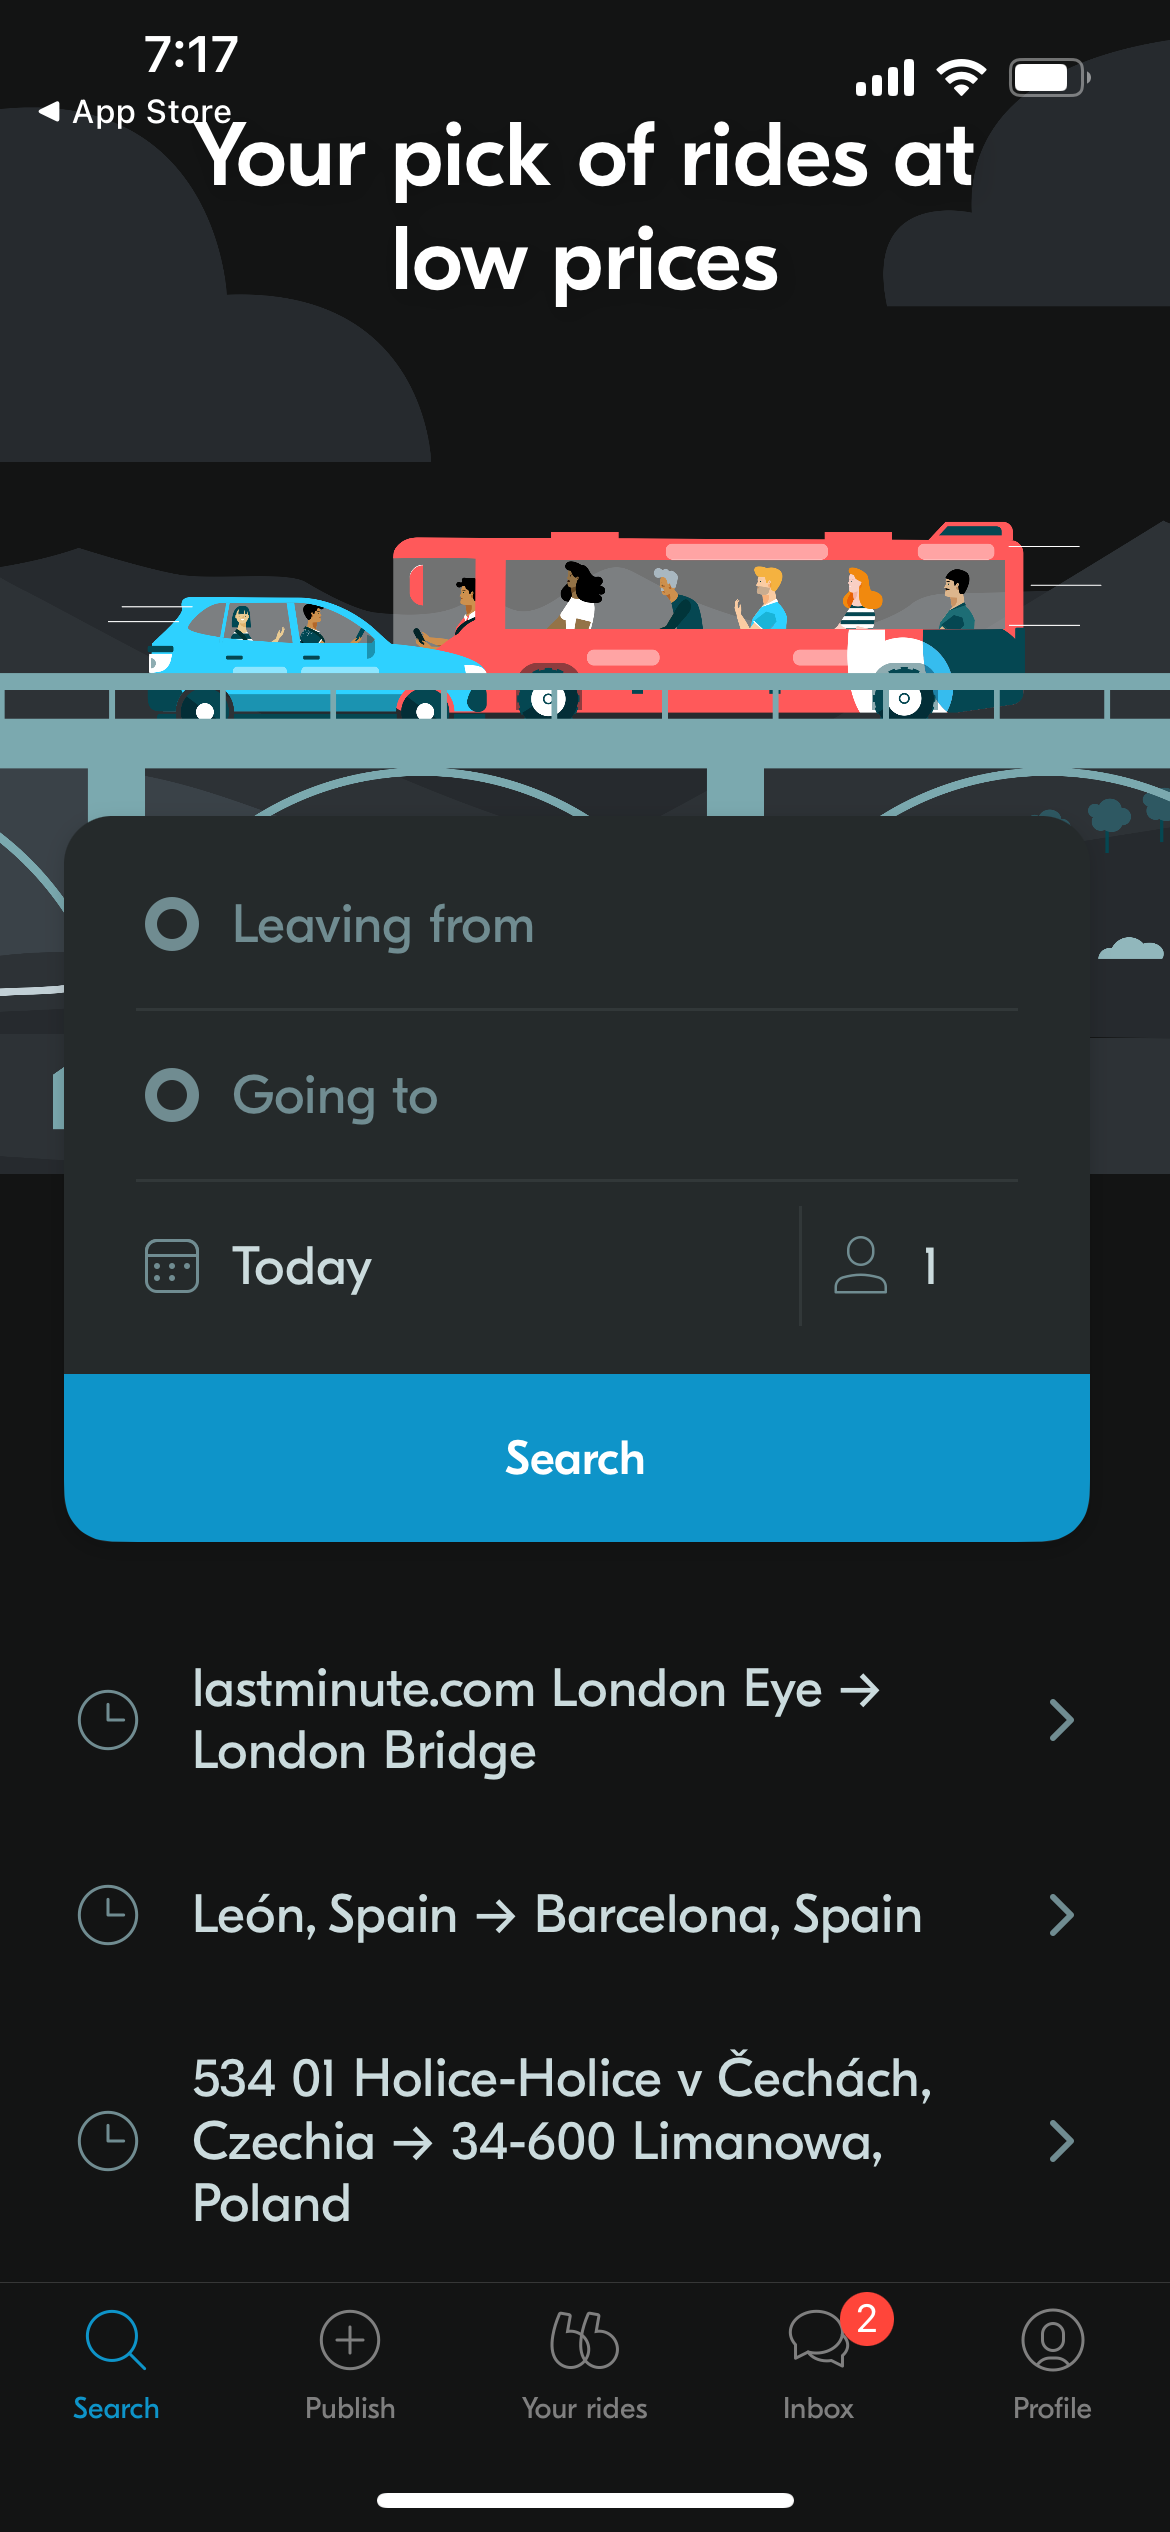
\includegraphics[width=0.8\linewidth, height=0.9\textheight, keepaspectratio]{Images/Blablacar_search.PNG}
                        \caption{Search Page}
                        \label{fig:blabla_search}
                    \end{subfigure}
                    \begin{subfigure}{0.3\textwidth}
                        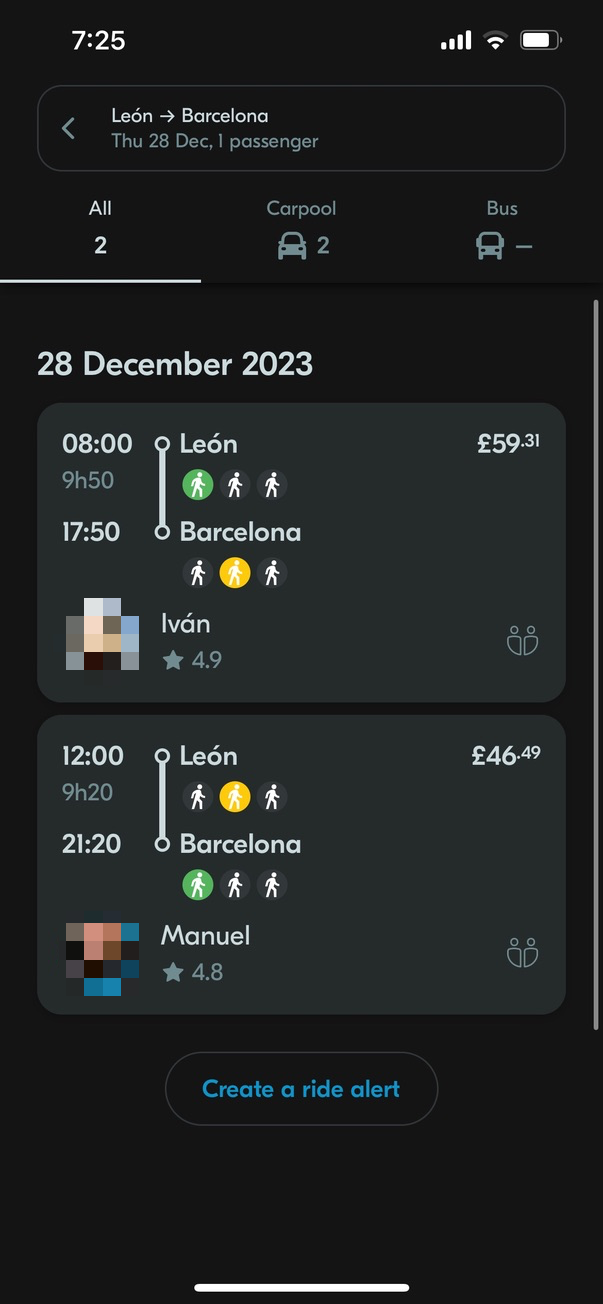
\includegraphics[width=0.8\linewidth, height=0.9\textheight, keepaspectratio]{Images/Blablacar_search_result.png}
                        \caption{Trip Search Results Screen}
                        \label{fig:blabla_results}
                    \end{subfigure}
                    \begin{subfigure}{0.3\textwidth}
                        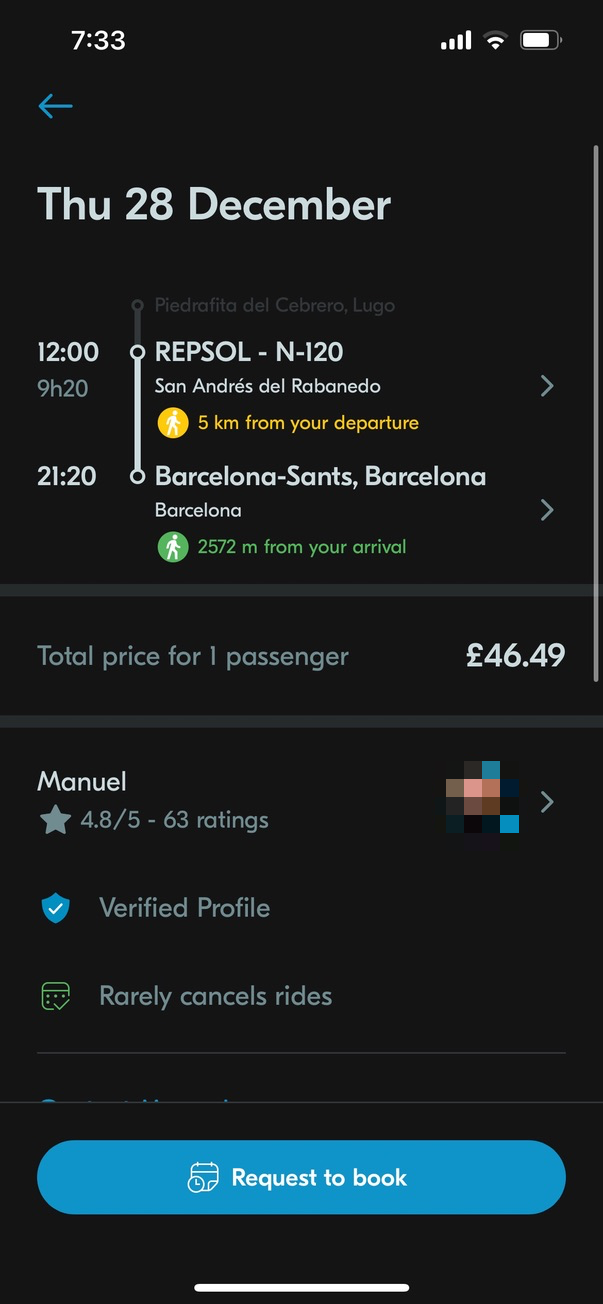
\includegraphics[width=0.8\linewidth, height=0.9\textheight, keepaspectratio]{Images/Blablacar_trip_detail.png}  
                        \caption{Trip Detail Screen}
                        \label{fig:blabla_detail}
                    \end{subfigure}
                    \newline % adding a vertical space between figures 
                    \newline
                    \begin{subfigure}{0.3\textwidth}
                        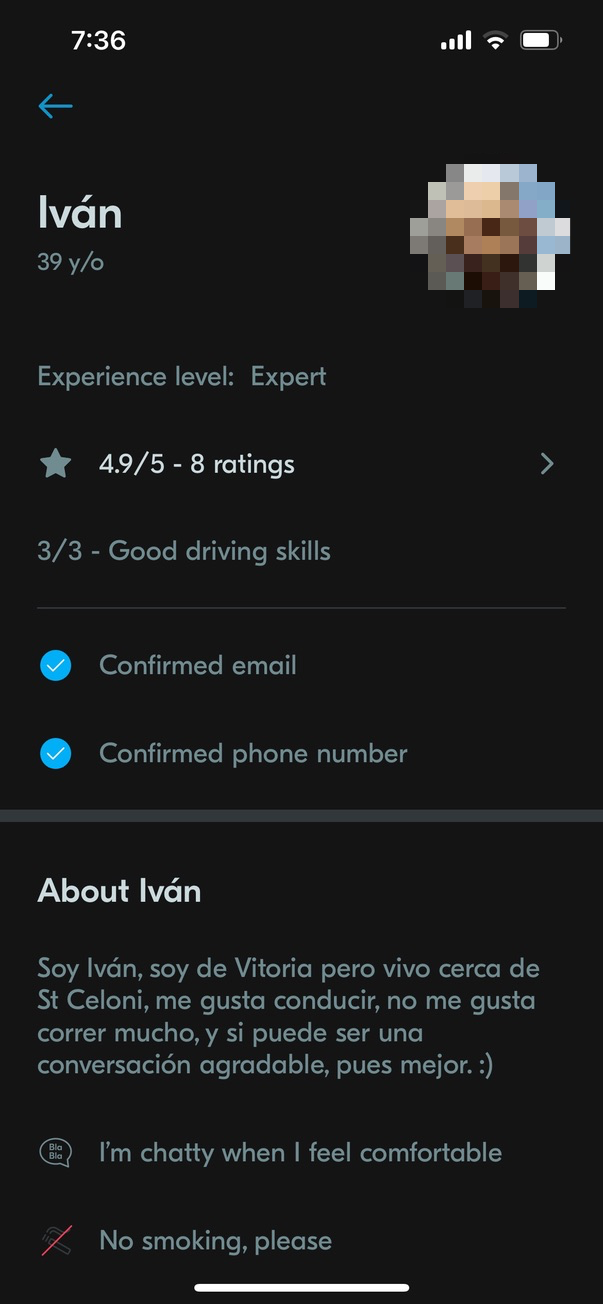
\includegraphics[width=0.8\linewidth, height=0.9\textheight, keepaspectratio]{Images/Blablacar_userprofile.png}
                        \caption{User Profile Screen}
                        \label{fig:blabla_profile}
                    \end{subfigure}
                    \begin{subfigure}{0.3\textwidth}
                        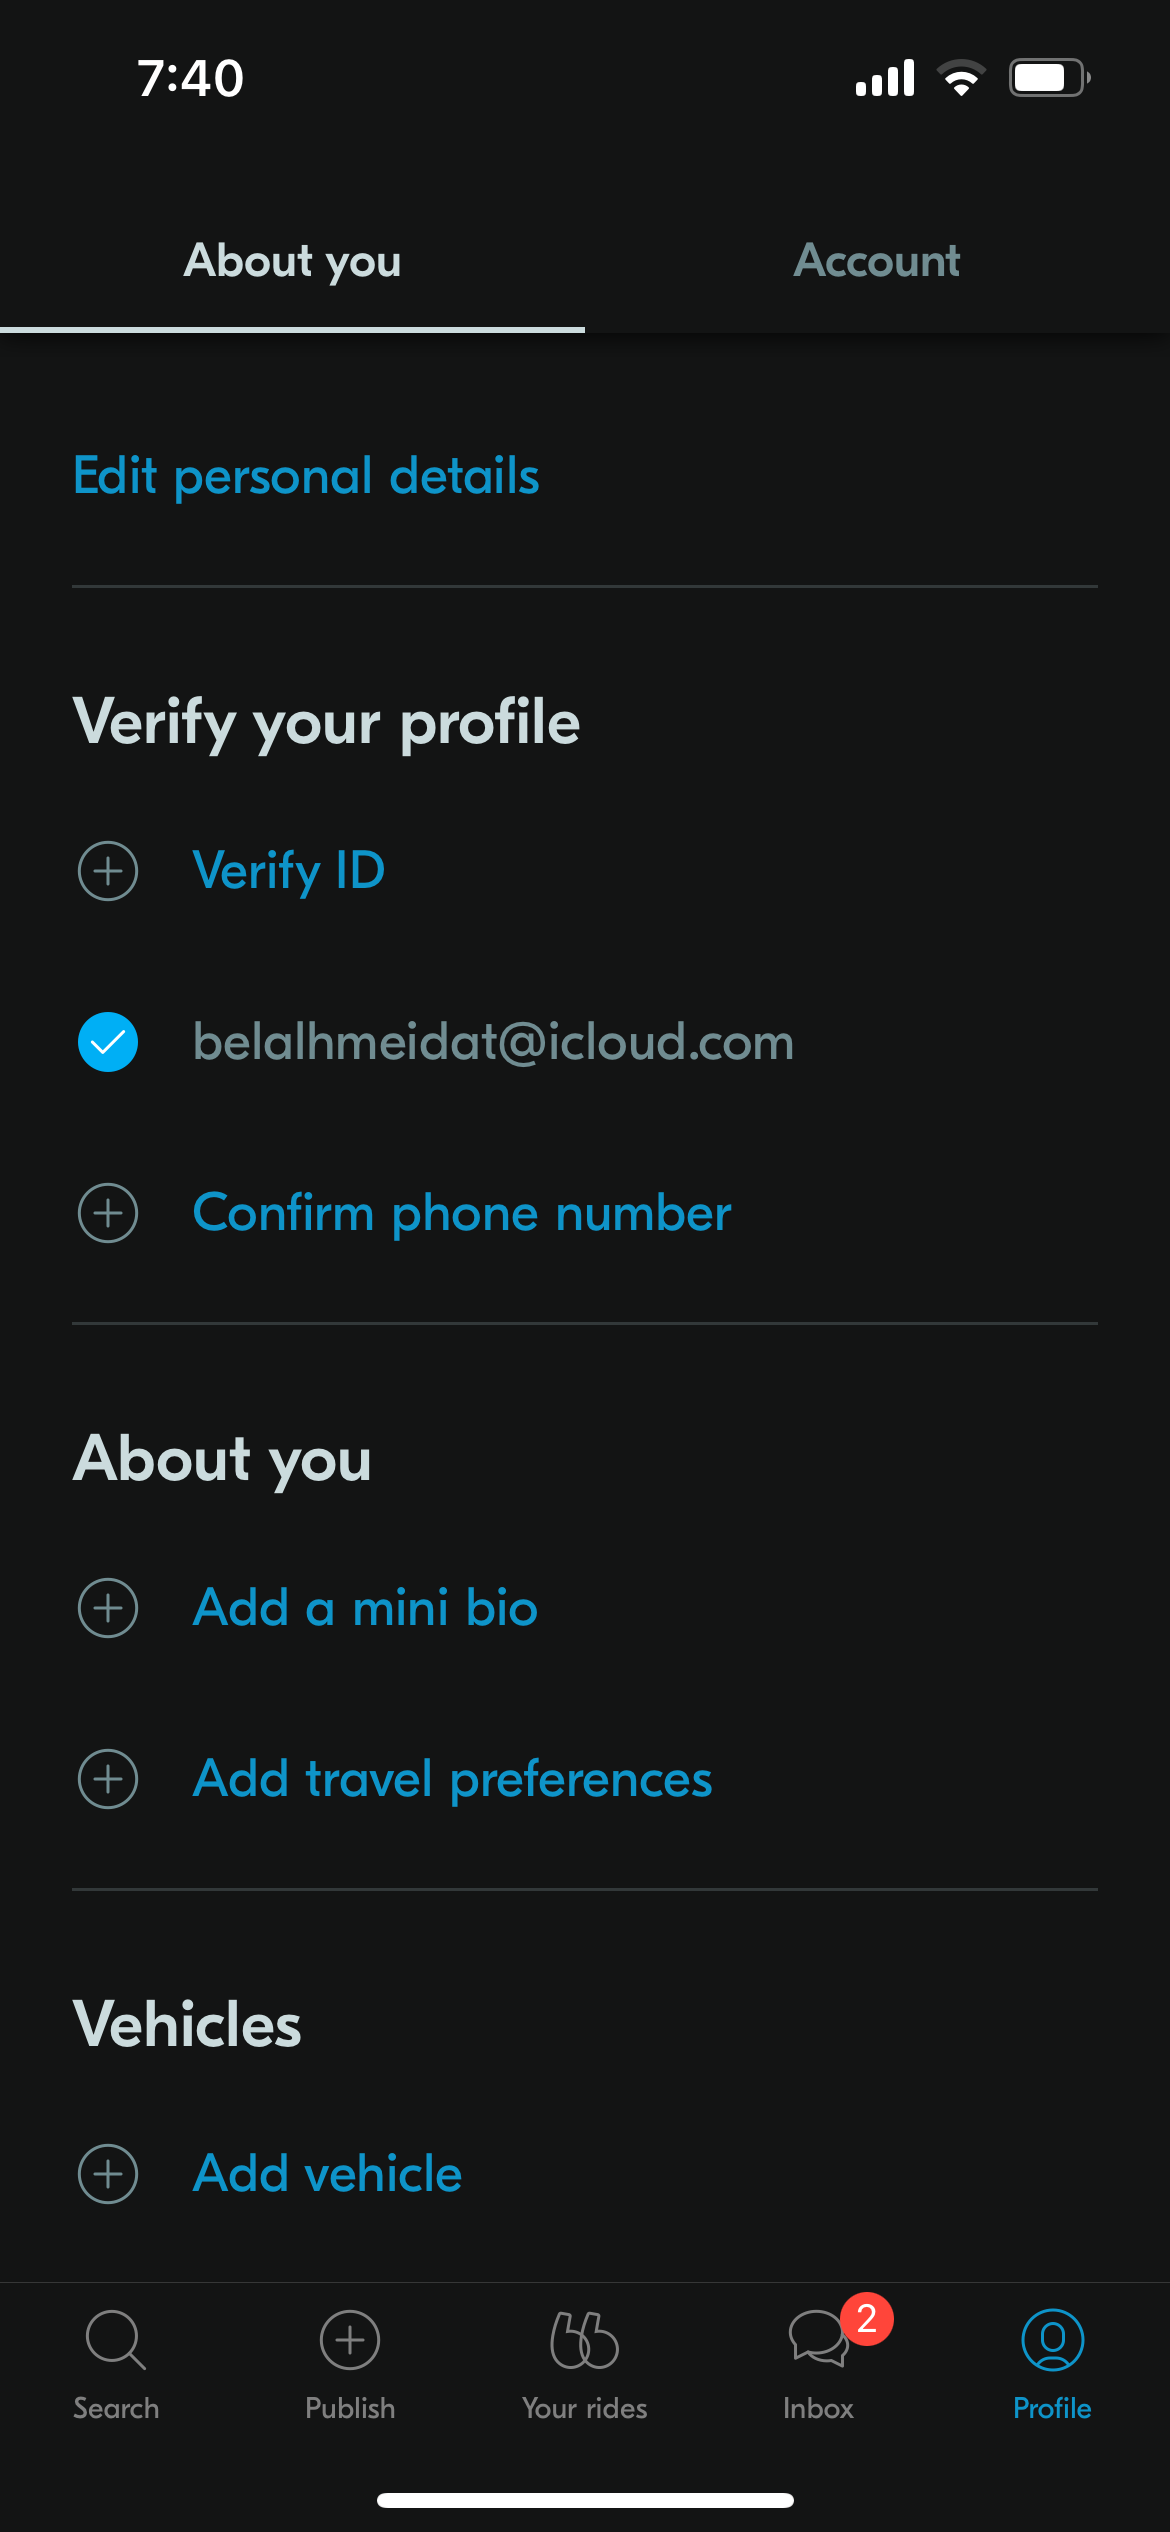
\includegraphics[width=0.8\linewidth, height=0.9\textheight, keepaspectratio]{Images/Blablacar_settings.PNG}
                        \caption{Settings Screen}
                        \label{fig:blabla_settings}
                    \end{subfigure}
                    \caption{BlaBlaCar App Pages Overview \cite{blablacar_app}}
                    \label{fig:blabla_gallary}
                \end{figure}
                \pagebreak
            \subsubsection{Gett}
                Also called Gett Taxi, which is a B2B Ground Transportation Management (GTM) platform, which was designed to help people save a lot of time and effort as it offers a faster, easier, and cheaper way for people to find transportation from one place to another. \cite{gett_wiki,gett_news} Gett is available and operating in Palestine particularly inside pre-1948 borders. The app offers many quality features such as being able to see drivers on the map and utilizing it to choose exact pickup and drop-off locations. Moreover, the app allows users to choose the type of ride and car size they want: shared ride, chauffeur, SUVs, and more. While being fairly popular around, the company's business model is primarily providing cab services rather than ride-sharing, hence the name Gett Taxi. It can offer a better experience for passengers going on long trips more than public transportation services do but it doesn't have other noteworthy advantages over them. 
                \begin{figure}[htp]
                    \centering
                    \begin{subfigure}{0.4\textwidth}
                        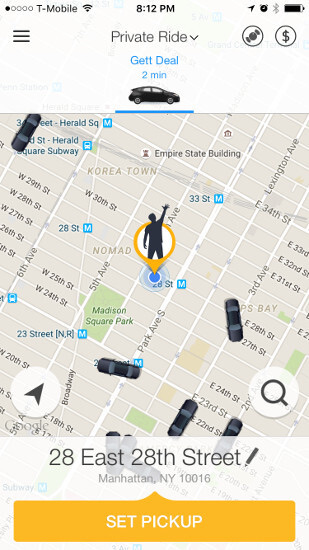
\includegraphics[width=0.8\linewidth, height=0.9\textheight, keepaspectratio]{Images/Gett_Map.jpeg}
                        \caption{Ride Location on Map}
                        \label{gett_map}
                    \end{subfigure}
                    \begin{subfigure}{0.4\textwidth}
                        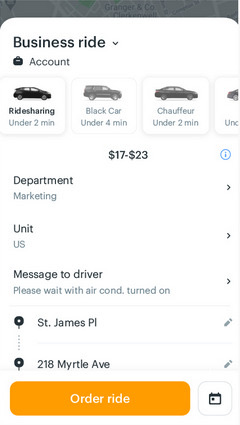
\includegraphics[width=0.8\linewidth, height=0.9\textheight, keepaspectratio]{Images/Gett_trip_detail.jpeg}
                        \caption{Trip Detail Screen}
                        \label{gett_detail}
                    \end{subfigure}
                    \caption{Pictures from withing Gett Taxi App \cite{gett_gallary}}
                    \label{fig:gett_gallary}
                \end{figure}
            \subsubsection{inDrive}
                International ride-hailing service and one of the most popular carpooling apps in the world. It sits as the second most downloaded ride-sharing and taxi app. \cite{indrive_wiki} In addition to being a taxi alternative, inDrive is used for many services such as courier delivery, freight transport, and professional services such as home repairs and tutoring. inDrive appeals to its user base by allowing them to negotiate a price with different drivers and thus helping them find the price they're looking for. The app itself allows users to select a service and select locations on the map. It also shows nearby drivers on the map. It also gives users access to message or start a call with the driver from within the app.\cite{indrive_itunes} Despite being very popular, inDrive is not available in Palestine. The business operates differently from BlaBlaCar and our app as it falls in line with the workflow of other famous carpooling apps such as Uber which is primarily a carpooling app that drivers rely on for bringing in income rather than merely sharing a ride. It also offers more general use cases such as professional maintenance services.
                \begin{figure}[h]
                    \centering
                    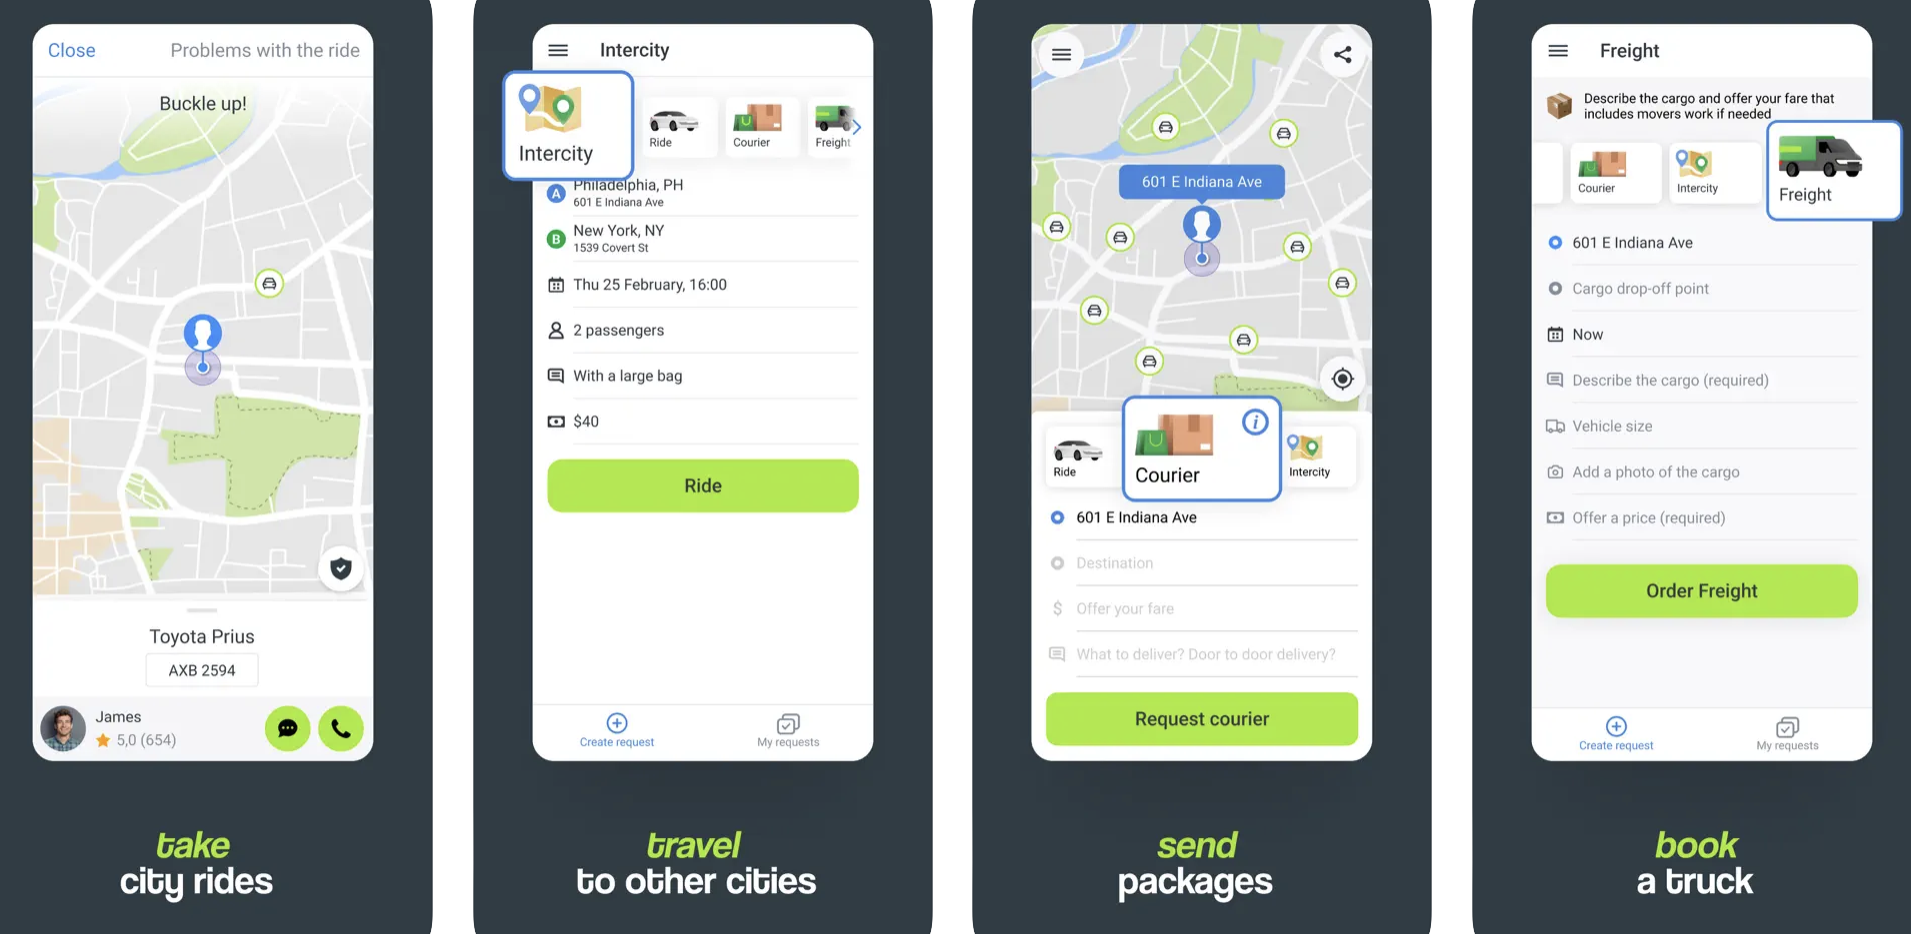
\includegraphics[width=0.9\linewidth]{Images/inDrive_Overview.png}
                    \caption{Screens showcasing inDrive app \cite{indrive_itunes}}
                    \label{indrvie_galary}
                \end{figure}
            \pagebreak    
            \subsubsection*{}
                Here is how they compare to our app:
                \newcolumntype{s}{>{\columncolor[HTML]{AAACED}} c}  % creating custom column type for Our App features column
                \renewcommand{\arraystretch}{1.5}  % increasing row height
                \begin{spacing}{1} % adjusting spacing between lines to lower value so that the table doesn't stretch too long. Text in the table has smaller line spacing due to this.
                   \begin{ThreePartTable}
                        \begin{TableNotes}
                        \footnotesize
                        \item [*] Feature is not of high priority. We will try to implement this feature if time allows but don't promise to.
                        \item [1] The passengers can see a list of drivers heading to their destination sorted by certain criteria as well as a map showing nearby locations of drivers in the list.
                        \item [2] location snapshots if live location feature is found not viable.
                        \item [3] Users can see the name and rating of a passenger who is on the same trip when browsing trips. They can visit their profiles after booking the trip.
                        \end{TableNotes}
                        \begin{longtable}{| >{\centering\arraybackslash}m{4cm} |c|c|c|s|}
                            \caption{Our app compared to similar other known apps.\label{comparisonTable}}\\
                            \rowcolor{gray} \textbf{Feature} & \textbf{inDrive} & \textbf{BlaBlaCar} & \textbf{Gett} & \textbf{\Large{Our App}}\\
                            \midrule
                            \endfirsthead

                            \caption*{Our app compared to similar other known apps (continued)}\\
                            \toprule
                            \rowcolor{gray} \textbf{Feature} & \textbf{inDrive} & \textbf{BlaBlaCar} & \textbf{Gett} & \textbf{\Large{Our App}}\\
                            \midrule
                            \endhead

                            \endfoot
                            \bottomrule
                            \insertTableNotes 
                            \endlastfoot
                            \hline
                            Anyone can make a trip after verification (no contract) 
                            & \checkmark & \checkmark & \checkmark & \Large{\checkmark}\\
                            \hline
                            Ability to pay beforehand through the app
                            & \checkmark & \checkmark & \checkmark & \Large{\checkmark}\\
                            \hline
                            Driver can schedule trips days prior
                            & \checkmark & \checkmark & & \Large{\checkmark}\\
                            \hline
                            Passengers can browse as a guest
                            & & \checkmark &  & \Large{\checkmark}\\
                            \hline
                            Passengers can filter through drivers
                            & \checkmark & & & \Large{\checkmark}\\
                            % \hline
                            % Users can set rules visible on their profile
                            % & & \checkmark & & \Large{\checkmark}\\
                            \hline
                            Cancellations allowed
                            & \checkmark & \checkmark & \checkmark & \Large{\checkmark}\\
                            \hline
                            \rowcolor{lightgray} \multicolumn{5}{|c|}{Pickup Locations} \\
                            \hline
                            Pickup on the way
                            & & & & \Large{\checkmark} (from stations) \\
                            \hline
                            List and map of trips from nearby locations\tnote{1}
                            & & & & \Large{\checkmark}\\
                            \hline
                            \rowcolor{lightgray} \multicolumn{5}{|c|}{Alternative routes} \\
                            \hline
                            Provide other trip suggestions to complete the trip\tnote{*}
                            & & & & \Large{\checkmark}\\
                            \hline
                            Provide public transportation station information to be able to complete the trip \tnote{*}
                            & & & & \Large{\checkmark}\\
                            \hline
                            \rowcolor{lightgray} \multicolumn{5}{|c|}{Map integration} \\
                            \hline
                            Trip route on the map
                            & & \checkmark & \checkmark & \Large{\checkmark} (limited)\\
                            \hline
                            Live location of drivers\tnote{2}
                            & \checkmark & & \checkmark & \Large{\checkmark}\\
                            \hline
                            \rowcolor{lightgray} \multicolumn{5}{|c|}{Comunication and Trip Sharing} \\
                            \hline
                            User profile with rules, cars, trip counting, and ratings
                            & \checkmark & \checkmark & & \Large{\checkmark}\\
                            \hline
                            Users can see other passengers' profiles in the same trip\tnote{3}
                            & & \checkmark & & \Large{\checkmark}\\
                            \hline
                            In-app chat for passengers and driver\tnote{*}
                            & \checkmark & \checkmark & & \Large{\checkmark}\\
                            \hline
                            Rating and feedback for both passengers and drivers
                            & & \checkmark & &\Large{\checkmark}\\
                            \hline
                        \end{longtable}
                    \end{ThreePartTable}

                \end{spacing}


        \subsection{Relevant Research}
            \subsubsection{Carpooling, Who, Why, and How}
                In his article about who and why people do carpooling, ROGER F. TEAL \cite{carpool_who_why_how} outlines some of the factors that make carpooling appealing to people or not. He mentions numerous statistics and research done combined with comprehensive analysis on the topic. While the article is based on the U.S. environment, there are general conclusions that can be drawn from the paper that serve as useful indicators to guide us in how we approach our app. One of which is his conclusion that socio-economic factors have little effect on one's propensity to carpool. This conclusion has been echoed multiple times by other researches he mentioned in his paper and ones that we came across in our further readings as well. That being said, he later states that people of lower income are more willing to carpool. The paper also suggests that women are more likely to carpool than men. He also brings up the agreement among researchers he mentions in his paper that carpoolers travel much bigger distances to work than people who commute alone. This might be the case for Palestine as well since examples of people carpooling with others going to their work in further cities are fairly common. This information is helpful since our app relies on stations of pickup. The range these stations cover should be larger if people are more inclined to carpool to far places. This will streamline the station selection to fewer stations that people can use reliably instead of creating many other substations that people would more likely use other traditional transport methods to get to. He also finds that the percentage of unrelated people who carpool together is larger than those who are related. This is to be expected as the chance of family members working in the same place or at the same time is unlikely. However, in Palestine, families are fairly larger than American families; so the difference between these two percentages might be smaller. There is still a sizeable percentage of people who carpool with unrelated people and could benefit from our app to find them. Moreover, Dr. Teal finds that the number of unrelated people carpooling is higher than that of internal carpooling, where people carpool with their relatives, by 2.25 to 2.63 people respectively. He finds that internal carpooling is incentivized by vehicle shortage whereas external ones are motivated primarily by cost burden.\cite{carpool_who_why_how} Since our app is mainly focused on external - non-related - carpooling, we will have to focus on ways to make the app cost-cutting, maybe by limiting the price people set or suggest a recommended price tag that is proportional to the travel cost.
                
            \subsubsection{What Motivates Carpooling}
                In their paper about what encourages people to carpool \cite{soton381789}, Jun Guan Neoh, Maxwell Chipulu, and Alasdair Marshall dive into the factors that affect people's willingness to carpool. They reviewed 908 papers from previous studies and filtered them down to 19 eligible articles to perform a meta-analysis on them. They summarize the literature on the carpooling field as "rich in studies but doubts remain about the generalisability of the results, making it difficult for policy makers to translate the findings into practice."
                Their research splits the factors affecting carpooling into internal individual and judgemental factors and external environmental and situational factors. Like Teal (1984) \cite{carpool_who_why_how} and many other publications on the topic, this research agrees that socio-demographics don't strongly influence carpooling.  One key point drawn from their research regarding socio-demographic factors and one which agrees with Teal (1984) \cite{carpool_who_why_how} is that women carpool more than women do. We don't know if this translates well to Palestine but we aim that our app will be usable for both men and women easily by taking some measures that are friendly with the gender rules in Palestine such as giving female users the ability to filter female drivers only. In terms of situational factors, the research also confirms the previously discussed findings that carpooling favors longer distances. It also claims that the inconvenience of waiting for other carpooling members can be a major factor in pushing away people from carpooling. We see that this issue might be exacerbated in our app since we are allowing drivers to pick up people on the way. We need to bring countermeasures that will make pickup easier and faster. One such measure is limiting the number of people a person can pick up. In addition to the ability of drivers and passengers to communicate and decide on a pickup location, we also discussed utilizing the map so passengers can send their exact pickup location from the start when requesting the trip to the driver who can, in return, agree or send a new waiting location for the passenger. As for judgemental factors, the research notes that psychological factors play a major role in making carpooling decisions. More so than socio-demographic factors. People feel more comfortable carpooling with their relatives and co-workers than when they are carpooling with strangers. Commuter privacy is also a big factor as carpoolers feel a sense of giving up some privacy and personal space when carpooling. However, since public transportation is very popular in Palestine, we feel carpooling will be just as acceptable in this regard as it offers similar, if not better, privacy levels. The study also points out that a sense of control can encourage people to carpool, we believe we can achieve this in our app by offering the option to find trips that agree with the user's set rules. We expect people's willingness to carpool can be negatively affected by their inclination to socialize. We are trying to mitigate the effect of this by designating a rule for chatting and socializing. We can also benefit from the fact that our app is oriented around picking up people along the way, which in turn, encourages shy people to participate knowing that other people will be on the trip with them providing them similar environment to familiar public transportation. Pollution is also a factor that encourages people to carpool according to this research but while reducing carbon footprints is one of our goals, we don't believe it is a major incentive for carpoolers in Palestine. Nonetheless, we see that traffic plays a similar role in encouraging people but we don't know to what extent since the traffic and road situation in Palestine can be abnormal most of the time. Moreover, the research results point out the important and the not-so-significant factors that affect carpooling. It finds that transportation costs, the number of employees in the carpooler's workplace, and finding potential partners have the biggest effect. Some other less important factors include the availability of carpooling lanes, fixed working schedules, and urban areas. Factors such as age, marital status, parking costs, parking availability, and being a university student,  have negligible effects on carpooling. \cite{soton381789} Overall, we believe this research gives very good insight for us to decide on how we implement certain aspects of our app and will try to make good use of it in this project and future works to come.

            \subsubsection{Carpooling Challenges}
                In their research paper on carpooling and its economic implications for drivers \cite{carpool_challenge}, Hai-Jun Huang, Hai Yang, and Michael G.H. Bell address the challenges associated with carpooling, including inconvenience for those with flexible hours, increased travel time, and concerns about privacy and independence. The study primarily focuses on the economic effects of carpooling, employing two main models: deterministic and stochastic.
                
                Where deterministic mode, explores passengers’ behavior and thoughts about carpooling, and driving alone modes under various scenarios, including no-tool equilibrium and social conditions. On the other hand, the stochastic model takes the path of logit-based modeling, considering different factors such as fuel cost, assembly cost, value of time, and traffic congestion.
                
                The research adopts three main approaches to studying carpooling which are: estimating ride-sharing potential, predicting ride-sharing demand, and considering demand and supply effects. Several numerical examples are shown in the paper that demonstrate the impact of carpooling on car trips for users, which indicates a decrease in the overall cost for both passengers and drivers.
                To conclude, this research provides valuable insights into the economic aspects of carpooling, showing users’ behavior and preferences, and offering a good understanding of the challenges and benefits that this mode of transportation can bring with it. \cite{carpool_challenge}
    \pagebreak

    \section{Approach}  
        \subsection{Methodology}
            To ensure an effective development process, we have adopted the Agile development methodology \cite{agile_method} as the software development process throughout our journey.
            
            Where we went through our project using iterative cycles, which allowed for flexible development process.

            Following the selection of the software development process, our intial step was conducting a survey in which we gathered data from what we believe could be potential users. This helped us understand user 
            expectations and desires for the application. Additionally we referenced the coparative analysis of existing carpooling applications which helped us identify areas of improvement and features that would make the application stand out.

            After understanding the user needs and market landscape, we dived into the system analysis phase. In this phase, we defined the system requirements and use cases, which helped us understand the system's functionality and how users will interact with it.
            in which then we moved to technologies selection, where we chose the technologies that best fit our project requirements and our team's expertise. As in this phase we decided to migrate from using Java Spring Boot to Firebase as our backend, with Flutter being kept as our front end technology.

            As we progressed, we made use of the existing system requirements both functional and non functional, in addition to referencing the diagrams, such as use case diagram. which helped us to align our development progress with a visually mapped system architecture and functionality.

            During the development phase we began by establishing the database and connecting it with the flutter application, followed by implementing user interfaces with their respective backend functionalities in parallel.while ensuring a robust and scalable architecture that can be easily maintained and extended in the future.

            Throughout the semester, we followed the Agile methodology, where each phase of the development was planned, implemented and tested in iterations, which allowed us to adapt to changes and feedback quickly, ensuring a robust and reliable development process.
            
            This methodology has proven to be effective in ensuring a smooth and efficient development process, allowing us to deliver a high-quality product that meets user expectations and requirements within the specified time frame.

        \subsection{Resources}
            \subsubsection{West Bank Cities Roads Dataset}
                A dataset of all the roads commonly used to commute from one Palestinian town or city to another in the West Bank. This will be used to define fixed stations that allow for passengers to be picked up along the way from towns and cities that drivers normally pass by to arrive at their destination. There is no already made database that we know of as of the writing of this draft, 08/02/2024. We are to ask the responsible parties for one or start collecting it ourselves. Due to the narrow time window of the project, the scope of operational routes, or the routes the app will work on, is reduced to a smaller area to use as proof of concept and a test case for development; we chose the route of Qalqilya - Ramallah for this, see the figure \ref{fig:testcase_route} showcasing possible routes and possible stations in between. We aim to scale the app's operational scope from this to the whole of the West Bank wherever possible.
                
                \begin{figure}[H]
                    \centering
                    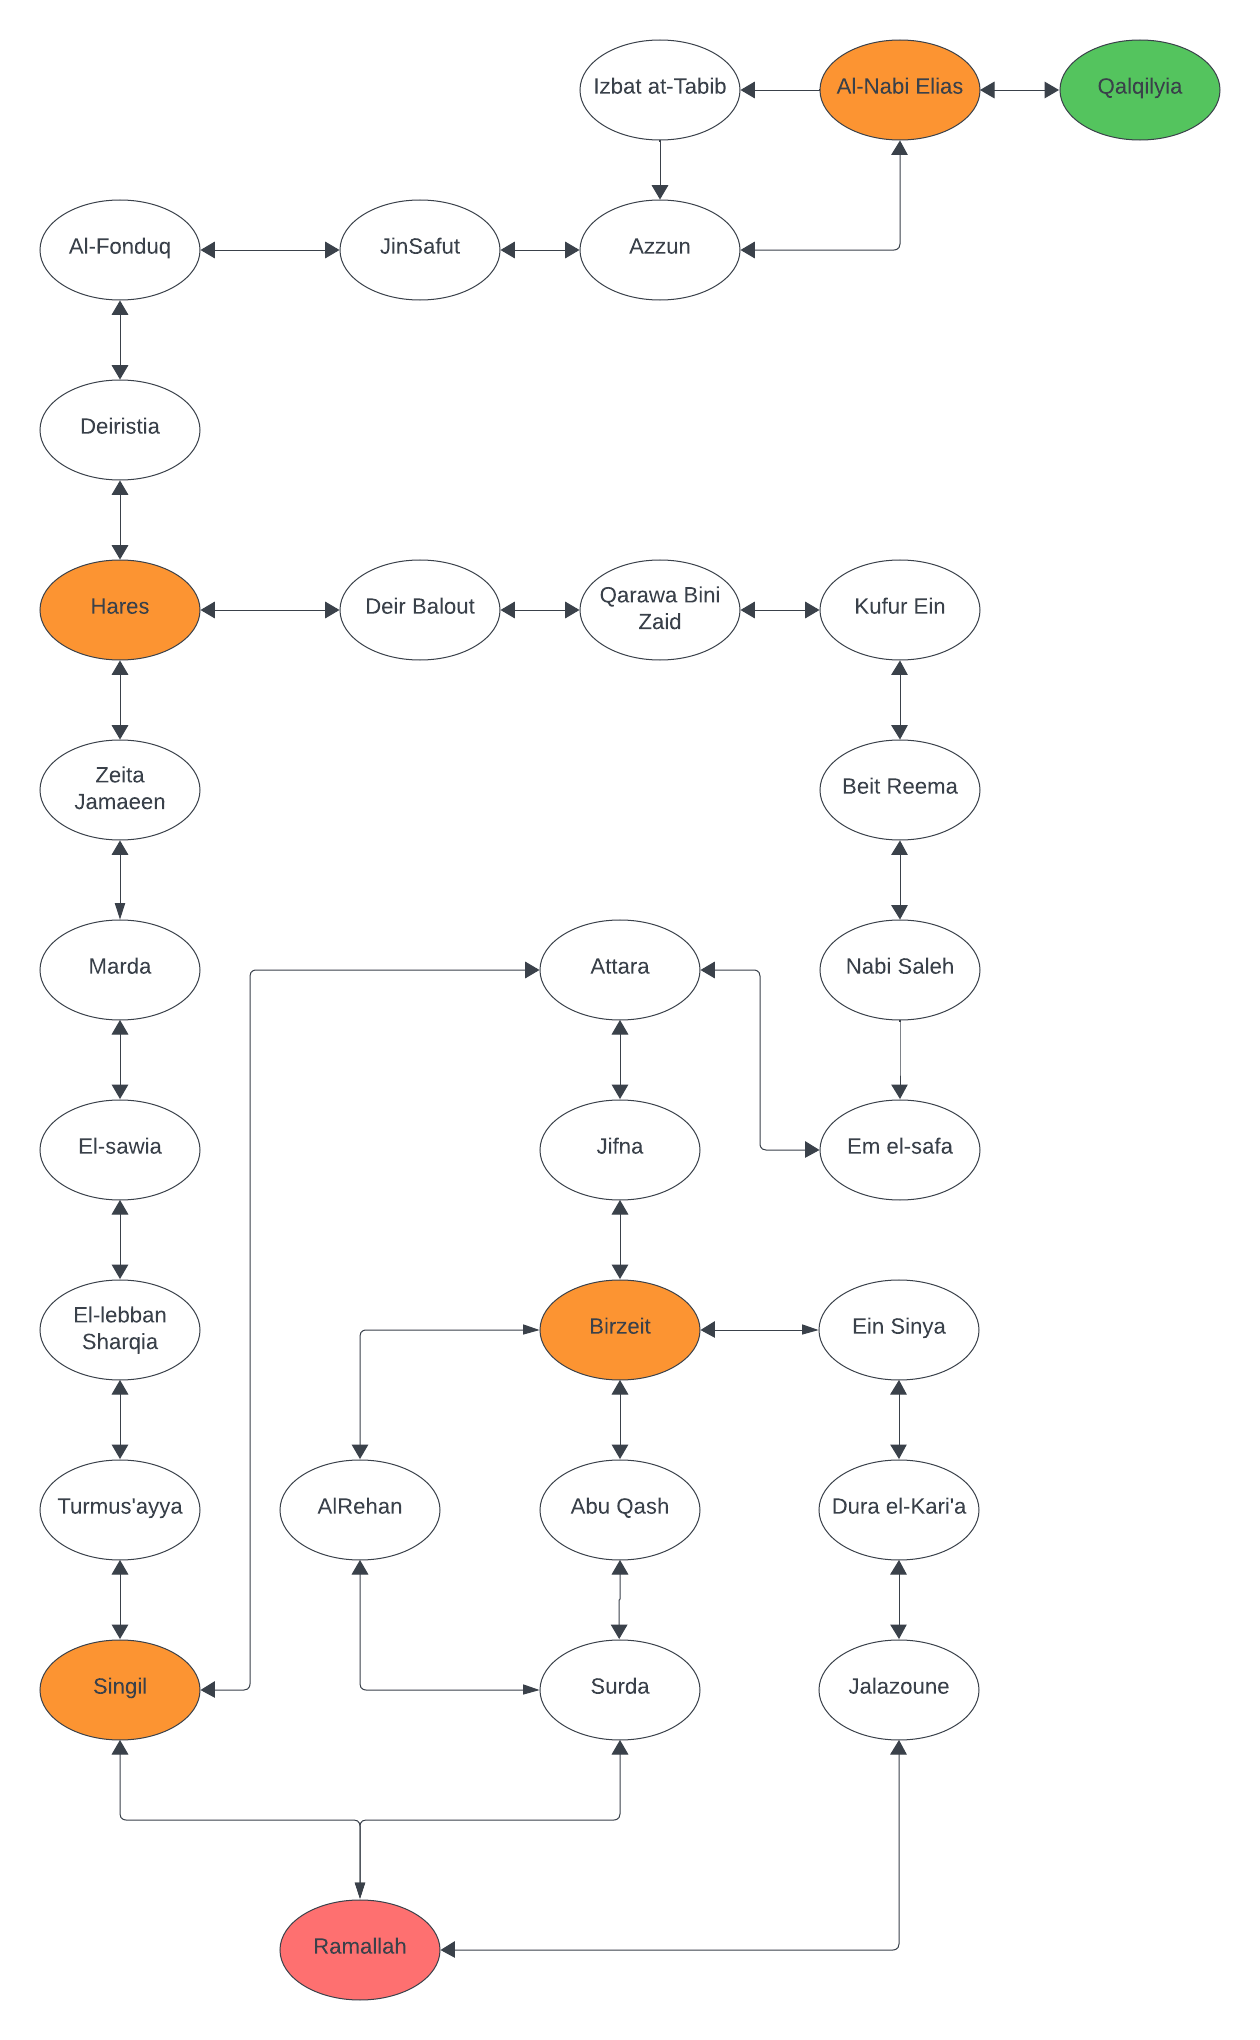
\includegraphics[width=0.7\textwidth, keepaspectratio]{Images/Route_Text_Case.png}
                    \caption{Test Case Route\protect \footnotemark[1]}
                    \label{fig:testcase_route}
                \end{figure}

                \footnotetext[1]{Orange denotes a branch.}
                \pagebreak
                
            \subsubsection{Public Opinion Questionnaire}
                A questionnaire to get public opinion on the idea. We assessed people’s acceptance of the idea, and whether they will partake in it as drivers or regular users, we took a look into their concerns and asked them for inputs and suggestions, which we took into consideration throughout the development phase.
            \subsection{Considerations}
                \subsubsection{User Privacy Consideration}
                    We will make sure the app respects user privacy. The app will be asking for user permission to access all needed device sensors and data such as camera access, location, calendar, and contacts if needed. It will not partake in collecting user data but for their necessary information such as phone number, real name, and payment method information. We will maintain the secrecy of this data and store it in a secure encrypted database. An in-app chat to allow passengers an easy channel with the driver is discussed. In case it is implemented we do not promise utilizing an end to end encrypted messaging. Lastly, users will be allowed the option to delete their accounts from our database at any time. 
                \subsubsection{Effect on Public Transportation Sector Consideration}
                    Our app is not meant to replace the public transportation sector and is not intended to be used as a main source of income for drivers. We have taken into consideration measures to combat that such as suspending accounts that do partake in that.
                \subsubsection{Legal Consideration}
                    In case of a reported felony or abuse committed by the driver or the passenger, we are willing to provide the driver's information to the legal authorities upon request. Access to users' (passengers and drivers) information can be acquired in case required by law. We are \textbf{not} to be held accountable for any of the drivers and passengers' actions.

        \pagebreak

        \subsection{Work Schedule}
            The implementation work plan clearly outlines the different stages needed to be completed to finish the project. Figure \ref{fig:work_plan} shows the work plan. The work plan starts with setting up the Firebase database with the collected sample routes, then moves to work on the trip scheduling logic and UI, then the trip booking logic and UI, then integrating the map and location services, then adding user profiles, user rules, trip filters, feedback, and rating features, then setting up the payment environment, then a polishing and fine-tuning phase.
            \begin{figure}[H]
                \centering
                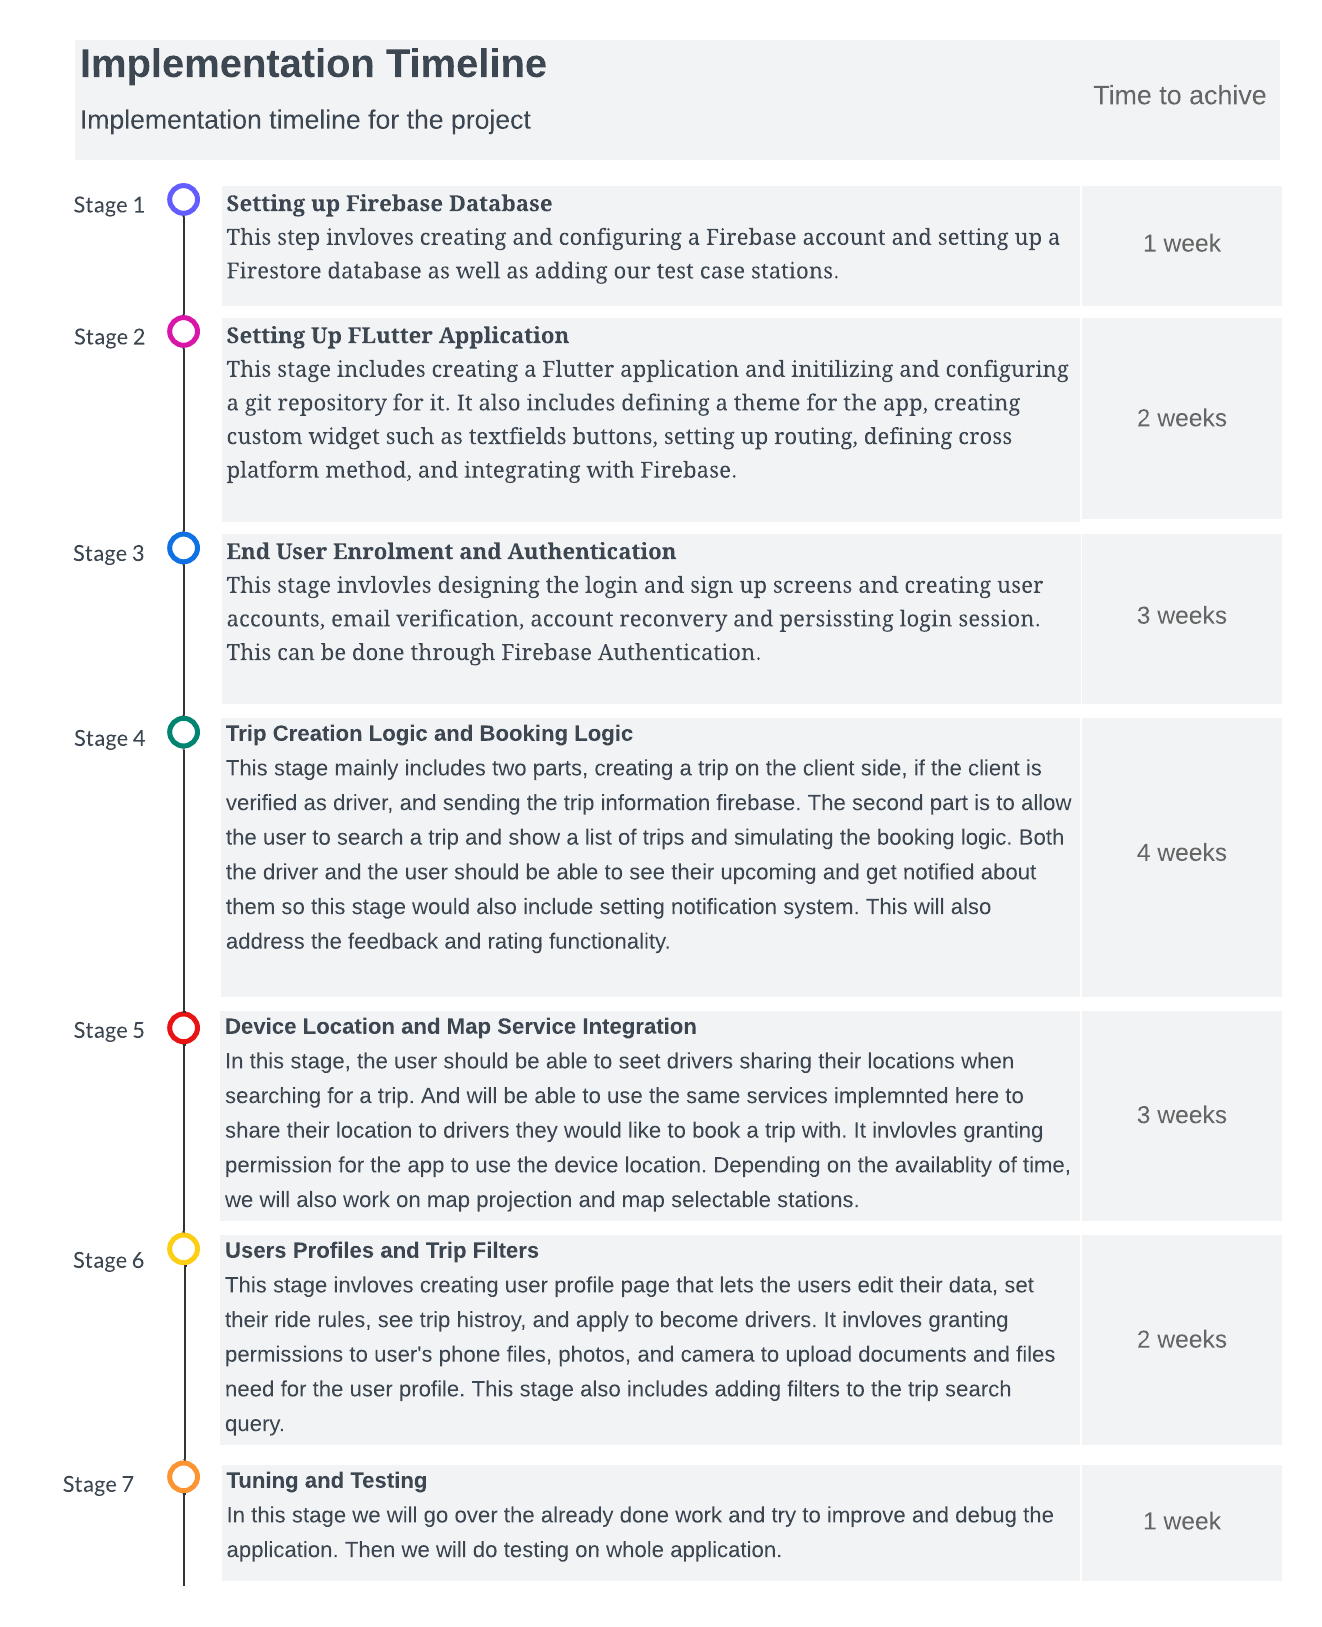
\includegraphics[width=0.9\textwidth]{Images/implemntation_timeline.png}
                \caption{Implementation Work Plan}
                \label{fig:work_plan}
            \end{figure}
        
    \pagebreak
    \section{System Analysis}  
        \subsection{Functional Requirements}
            Below are the details of all the user functional requirements (UR) and system requirements (SR) accompanying them.
           \begin{itemize}
                \item [$ $] UR1. Users shall be able to log in and log out after creating an account.
                \begin{itemize}
                    \item [$ $]SR1.1 The system shall allow users to sign up for the same type of account through the same page and app.
                    \item [$ $]SR1.2 The system shall enable both drivers and passengers to log in, with the ability to stay logged in till logout is requested.
                \end{itemize}
                \item [$ $] UR2. User shall have a profile where they can edit personal information, and add a set of rules for their trips.
                \begin{itemize}
                    \item [$ $] SR2.1 The system should allow the user to add/edit their personal information.
                    \item [$ $] SR2.2 The system should allow users to choose from a variety of rules to add to their trip preferences, such as smoking, music, etc.
                \end{itemize}
                \item [$ $] UR3. Users shall search for trips by selecting the departure location, destination, and date for a trip as a member/guest.
                \begin{itemize}
                    \item [$ $] SR3.1 The system shall look for drivers going to the selected destination on the same date and passing by the user’s departure location.
                    \item [$ $] SR3.2 The system shall display relevant trip details, including driver information, route, and rules, and expected arrival time. 
                    \item [$ $] SR3.3 The system shall sort the drivers list depending on the time and route taken whether they respect the user’s set rules or not.
                    \item [$ $] SR3.4 The system shall allow users to browse trips without signing in (as guests).
                    \item [$ $] SR3.5 The system shall display a list of trips based on the user's given requirements.
                    \item [$ $] SR3.6 The system shall provide locations of nearby drivers making the requested trip on a map mirroring the information provided in the list. 
                \end{itemize}
               \item [$ $] UR4. Users should be able to become drivers after undergoing a verification process. 
               \begin{itemize}
                   \item [$ $] SR4.1 System shall allow users with cars willing to collect passengers along their way to undergo a verification process to become verified drivers.
                    \item [$ $] SR4.2 The system shall notify the Users if they were accepted or not.
               \end{itemize}            
                \item [$ $] UR5. Admins shall be notified about new applying Drivers.
                \begin{itemize}
                    \item [$ $] SR5.1 The system shall send a notification to the responsible department about newly applied drivers
                    \item [$ $] SR5.2 The responsible department shall evaluate the user’s request and approve or deny their request. 
                \end{itemize}
                \item [$ $] UR6. Users shall be able to file complaints and reports which shall be received by the responsible department to resolve issues or provide support.
                \begin{itemize}
                    \item [$ $] SR6.1 The system shall notify Admins about drivers’ being reported more than 3 times.
                    \item [$ $] SR6.2 The admins can review the complaints and take action if they are valid complaints.
                \end{itemize}
                \item [$ $] UR7. Verified drivers shall be allowed to schedule trips.
                \begin{itemize}
                    \item [$ $] SR7.1 The system shall allow drivers to schedule trips by selecting the departure and destination locations and time of the trip.
                    \item [$ $] SR7.2  The system shall ask the driver to specify available seats and luggage rooms.
                    \item [$ $] SR7.3  The system should allow the driver to select the route throughout the trip.
                \end{itemize}
                \item [$ $] UR8. Users shall be able to report other users (drivers/ passengers) for any complaints. 
                \begin{itemize}
                    \item [$ $] SR8.1 The system shall allow passengers to report drivers 
                    \item [$ $] SR8.2 The system shall allow drivers to report passengers.
                    \item [$ $] SR8.3 The system shall allow passengers to report each other if they were on the same trip.
                    \end{itemize}
                \item [$ $] UR9. Users shall be able to give feedback and ratings to different users.
                \begin{itemize}
                    \item [$ $] SR9.1 The system shall allow passengers to provide feedback and ratings for their driver.
                    \item [$ $] SR9.2  The system shall allow drivers to provide feedback and rating for their passengers.
                    \item [$ $] SR9.3 The system shall allow passengers to provide feedback and ratings to other passengers on the same trip.
                \end{itemize}
                \item [$ $] UR10. Passengers shall be able to book trips.
                \begin{itemize}
                    \item [$ $] SR10.1 The system shall allow only signed-in members to book trips.
                    \item [$ $] SR10.2  The system shall display relevant trip details, including driver information, route, and set rules. 
                    \item [$ $] SR10.3 The system shall notify the driver of this booking.
                    \item [$ $] SR10.4 The system should wait for the driver to accept the request before confirming the booking.
                    \item [$ $] SR10.5 The system shall request the passenger to pay for the trip.
                \end{itemize}
                \item [$ $] UR11. Passengers shall be able to pay for the trip.
                \begin{itemize}
                    \item [$ $] SR11.1 The system shall allow passengers to pay through different online payment methods.
                    \item [$ $] SR11.2The system shall complete the payment securely.
                    \item [$ $] SR11.3 The system shall confirm the booking for the driver/passenger.
                    \item [$ $] SR11.4 The system shall complete the payment for the driver when trip end confirmation is done.
                \end{itemize}
                \item [$ $] UR12. Users shall be able to cancel trips (Both Drivers and passengers’) and get refunds.
                \begin{itemize}
                    \item [$ $] SR12.1 The system shall allow users to cancel the trip.
                    \item [$ $] SR12.2 The system shall start the refund process for this trip.
                    \item [$ $] SR12.3 The system shall notify the driver/passengers when cancellation is completed.
                    \item [$ $] SR12.4 The system shall calculate the refund based on the time of the cancellation.
                    \item [$ $] SR12.5 The system should allow for a full refund if the driver is too late from his planned arrival time.
                \end{itemize}
                \item [$ $] UR13. The passenger shall be notified sometime before the driver's scheduled/ estimated arrival time.
                \item [$ $] UR14. Users (driver and passenger) should confirm that the trip is finished and will have the option to provide feedback when the trip is complete.
                \begin{itemize}
                    \item [$ $] SR14.1 The system should receive confirmation from both the driver and passenger at the end of the trip. 
                    \item [$ $] SR14.2 The system will prompt the driver to rate the passenger. 
                    \item [$ $] SR14.3 The system shall prompt the passenger to rate the trip, the driver, and other passengers. 
                \end{itemize}
                \item [$ $] UR15. The user shall be able to change their account’s settings e.g. change email, password, and privacy settings.  
           \end{itemize}
        \subsection{Non-Functional Requirements}
        \begin{enumerate}
            \item The app must submit to the average acceptable response time for mobile apps which is 2-3 seconds.
            \item The app must be reliable, this means that it must work correctly at 97\%, and have a 3\% downtime. This means 12 hours of downtime per year.
            \item The app must submit to the industry standards security practices to protect collected and analyzed data.
            \item The app must be designed with well-documented code to allow future maintenance and enhancements.
            \item The app must be compatible with widely used Android and iOS versions, namely Android 10, iOS 13, and later.
            \item The app must feature an intuitive UI that is easy to use and navigate.
            \item The app must be scalable such as it can support the ability to scale the program in the future to keep up with rising demand.
            \item The app must be recoverable, as the database will be backed up with scheduled plans.
        \end{enumerate}
    \subsection{Use Cases}
        \subsubsection{Actors Description}
            \begin{itemize}
                \item Admin: This actor is responsible for verifying drivers, and reviewing reports/complaints from app users.
                \item Driver: This actor is responsible for scheduling trips, accepting passengers to his trip, and operating the trip.
                \item Passenger: This actor can search for trips, and request to join trips that are available on the application.
                \item Guest User: This actor can download the application, but is limited to only searching for trips and seeing them (can not request to join trips).
            \end{itemize}
        \subsubsection{External Actors Description}
            \begin{itemize}
                \item Notification Manager: This service handles notifying actors about events such as informing admins of a newly filed report/ complaint from users, notifying admins about new requests from users wishing to become drivers, informing drivers of new ride requests from passengers, and reminding drivers and passengers of their upcoming trips.
                \item Map Services: This service is fired up whenever a new trip is added with its final destination located on the map, passenger checks to see a driver’s live location on the map, or when passengers choose a point on the map to be picked up from and the driver approves or sends back a different point for pick up.
                \item Payment Services: This service is responsible for facilitating payments between passengers and drivers. It is used whenever a payment transaction is made.
            \end{itemize}
        \subsubsection{Use Cases Description}
            This is a description of the use cases shown in \ref{fig:usecase}.
            \begin{enumerate}
                \item Login/ Registration \\
                    Actors: Driver, passenger \\
                    The page users are welcomed the first time they launch the app. It also offers an option to browse trips in guest mode.
                \item Login/Registration Verification\\            
                    Actors: Driver, passenger\\
                    When a user signs up for a new account, they are required to verify their phone number and email. When they sign in, a verification code is sent to their confirmed phone number
                \item Create an Account \\
                    Actors: Unregistered users\\
                    An unregistered user can create an account by entering the needed information: email, phone number, and password.
                \item Login \\
                    Actors: Driver, passenger\\
                    A user can log in by entering his email and password to the login page.
                \item Logout\\
                    Actors: Driver, passenger\\
                    A registered user can log in by clicking the logout button on the main screen.
                \item Become Verified \\
                    Actors: Driver, Passenger\\                
                    Users can choose to upload a picture of their ID card to earn a verified account badge. This serves as a measure to increase other user's trust in them. 
                \item Show/Edit Profile \\
                    Actors: Driver, passenger \\
                    A user can see his profile details, and edit them from adding preferences to his trips to updating their name and profile picture. They can also view their trip history from their profile or apply to become drivers. 
                \item Apply to Become Driver \\
                    Actors: passenger \\
                    A passenger can apply to become a registered driver by uploading their car registration, and their driving license, which then is revised by the admins.
                \item Notify driver about approval/decline for his application \\
                    Actor: notification manager \\
                    The notification manager should send a notification to the user to notify them about their driver’s application being approved or declined by the admin.
                \item Upload Driver Documents \\
                    Actors: Passenger\\
                    A driver needs to submit certain documents to prove eligible to start making trips. These documents are their driver's license and their car license. They are also required to take a photo of their face to undergo a verification process after they are sent to the admins. 
                \item Notify Admins about new Drivers \\
                    Actors: Notification Manager \\
                    The notification manager is responsible for notifying admins about new driver applications.
                \item Unlock Driver Features \\
                    Actors: admin \\
                    When a user’s submitted paper to become a driver is approved by the admin, the driver will unlock the ability to schedule trips for other users to book.
                \item Notify Users of Approved or Decline Requests \\
                    Actors: Admin, Notification Manager \\
                    When a user’s request to become a driver is examined by admin and approved or declined, the user will get a notification back telling him about the decision and the reasons behind refusal in case of one.
                \item Add Payment method \\
                    Actors: Passenger, Driver \\
                    The User can choose his preferred payment method that is presented in the application for future payments.
                \item Report/ Submit Complaint \\
                    Actors: Passenger, Driver \\
                    The user can report/submit a complaint about another user if he has recently been on a trip with them.
                \item Notify About Upcoming Trips \\
                    Actors: Notification Manager, Passenger, Driver \\
                    The notification manager is responsible for reminding a passenger/driver about their upcoming trips before a reasonable amount of time.
                \item Show Scheduled Trips \\
                    Actors: Driver, passenger \\
                    Drivers and passengers can see a page with their upcoming trips sorted by the time they are scheduled to start. 
                \item Manage Account Settings\\ 
                    Actors: Driver, passenger\\
                    Driver and passengers can access their account settings through the app to manage settings like changing their email, password, and payment method.
                \item Search Trips \\
                    Actors: passenger, Driver, Guest \\
                    Drivers, passengers, and application guests can search for trips by entering the departure, destination, and time of the trip he is looking for.
                \item View available trips \\
                    Actors: Driver, passenger, guest \\
                    Drivers, passengers, and application guests can view available trips after searching for them.
                \item Apply Trip Filter/ Sorting if Any \\
                    Actors: Driver, passenger, guest \\
                    Driver, passengers, and guests can filter their trip search results based on different criteria, such as driver rating, rules they would like the trip to abide by, or the verified status of the drivers.
                \item Show Chosen Trip Details \\ 
                    Actors: Driver, Passenger, Guest \\ 
                    Users searching for a trip can see more details about available trips, like driver information and rating, driver’s rules, names of other passengers on the trip and their ratings, and access to the driver profile from there.
                \item Schedule Trips \\
                    Actors: Driver, Map Service \\
                    The driver can schedule a trip by adding departure, destination, and time of the trip, preferred routes, and additional trip rules.
                \item Set trip route \\
                    Actors: Driver, Map Service \\
                    The driver can select the trip route using predefined stations allowing passengers to be picked up along the way. If the driver chooses not to select the routes, their trip will show up only to passengers coming from the same starting destination and going to the same final destination.
                \item Suggest New Stations \\
                    Actors: Driver, Map Service \\
                    The driver can suggest a new station to be added to the set of stations throughout a certain route.
                    
                \item Validate Trip \\
                    Actors: Driver \\
                    The system checks if the scheduled trip by the driver doesn't conflict with other trips they already set up. 
                \item Request to Join Trip \\
                    Actors: Driver, passenger \\
                    Driver and passenger can send a request to the trip driver to book a seat on the trip.
                \item Validate Request \\
                    Actors: passenger \\ 
                    A user’s request to join a trip is validated so that it does not conflict with other scheduled Trips.
                \item Review Join Trip Request \\
                    Actors: Driver \\
                    The driver can see requests from passengers wanting to ride with them and accept or decline depending on the ratings of the passenger, and other factors such as the verified account status of the passenger and their location. 
                \item Notify Passenger of Driver Response to Trip Request\\
                    Actors: Driver, Notification Manager\\
                    When a driver accepts or declines a passenger’s request to be picked up, the system notifies the passenger and enables them to proceed to payment in case of approval.
                \item Send Payment to Driver for Trip\\
                    Actors: payment service, Admin\\
                    At the end of trip confirmation, The system processes the payment to the driver's account.
                \item Receive Payment\\
                    Actors: payment Service, Admin\\
                    When a payment is made by a passenger the payment service transfers the money into a median pocket owned by the application admins which holds the payment until trip completion.
                \item Confirm Trip Completion\\
                    Actors: Driver, passenger\\
                    At the end of the trip: \\
                        The driver should ask and ensure that the passenger confirms that his trip has ended. \\
                        The driver should confirm that the trip has ended when he reaches his destination.
                \item Cancel a Reservation\\
                    Actors: passenger\\
                    passengers are allowed to cancel a trip reservation within a limited amount of time estimated xx hours, with a full refund, and a partial refund accounted for the remaining time of the trip after that.
                \item View Accepted Trips\\
                    Actors: Passenger\\
                    Passengers can view the trips that they have been accepted to and decide which one they are going to attend.
                \item Perform Payment \\
                    Actors: Passenger, Payment Service \\
                    Passenger can pay for the trip they have chosen to attend and their seat is booked on successful payment. Additionally, all previous requests sent to other drivers will be canceled.
                \item Validate Payment \\
                    Actors: Payment Service \\
                    The payment service is responsible for validating the payment and transferring the money from the passenger to the admin’s account.
                \item Cancel a Reservation\\
                    Actors: Passenger \\
                    The passenger is allowed to cancel an already booked trip or a trip request. If the trip is paid for, a refund is issued back to the passenger’s payment method. The refunded amount will be deferred depending on how late the passenger requests to cancel.
                \item Ask for Rating/ Feedback\\
                    Actors: Passenger, Driver\\
                    On the trip's end, both passengers and drivers are able to rate each other and provide feedback if they wish.
                \item View trip history \\
                    Actors: Passenger, Driver \\
                    Passengers and drivers can see their trip history from their profile section, and if a user is registered as a driver he can choose to display trips he made or trips he has been part of.
            \end{enumerate}
        
        \pagebreak
        \subsubsection{Use Case Diagram}

            \begin{figure}[H]
                \centering
                \makebox[\textwidth][c]{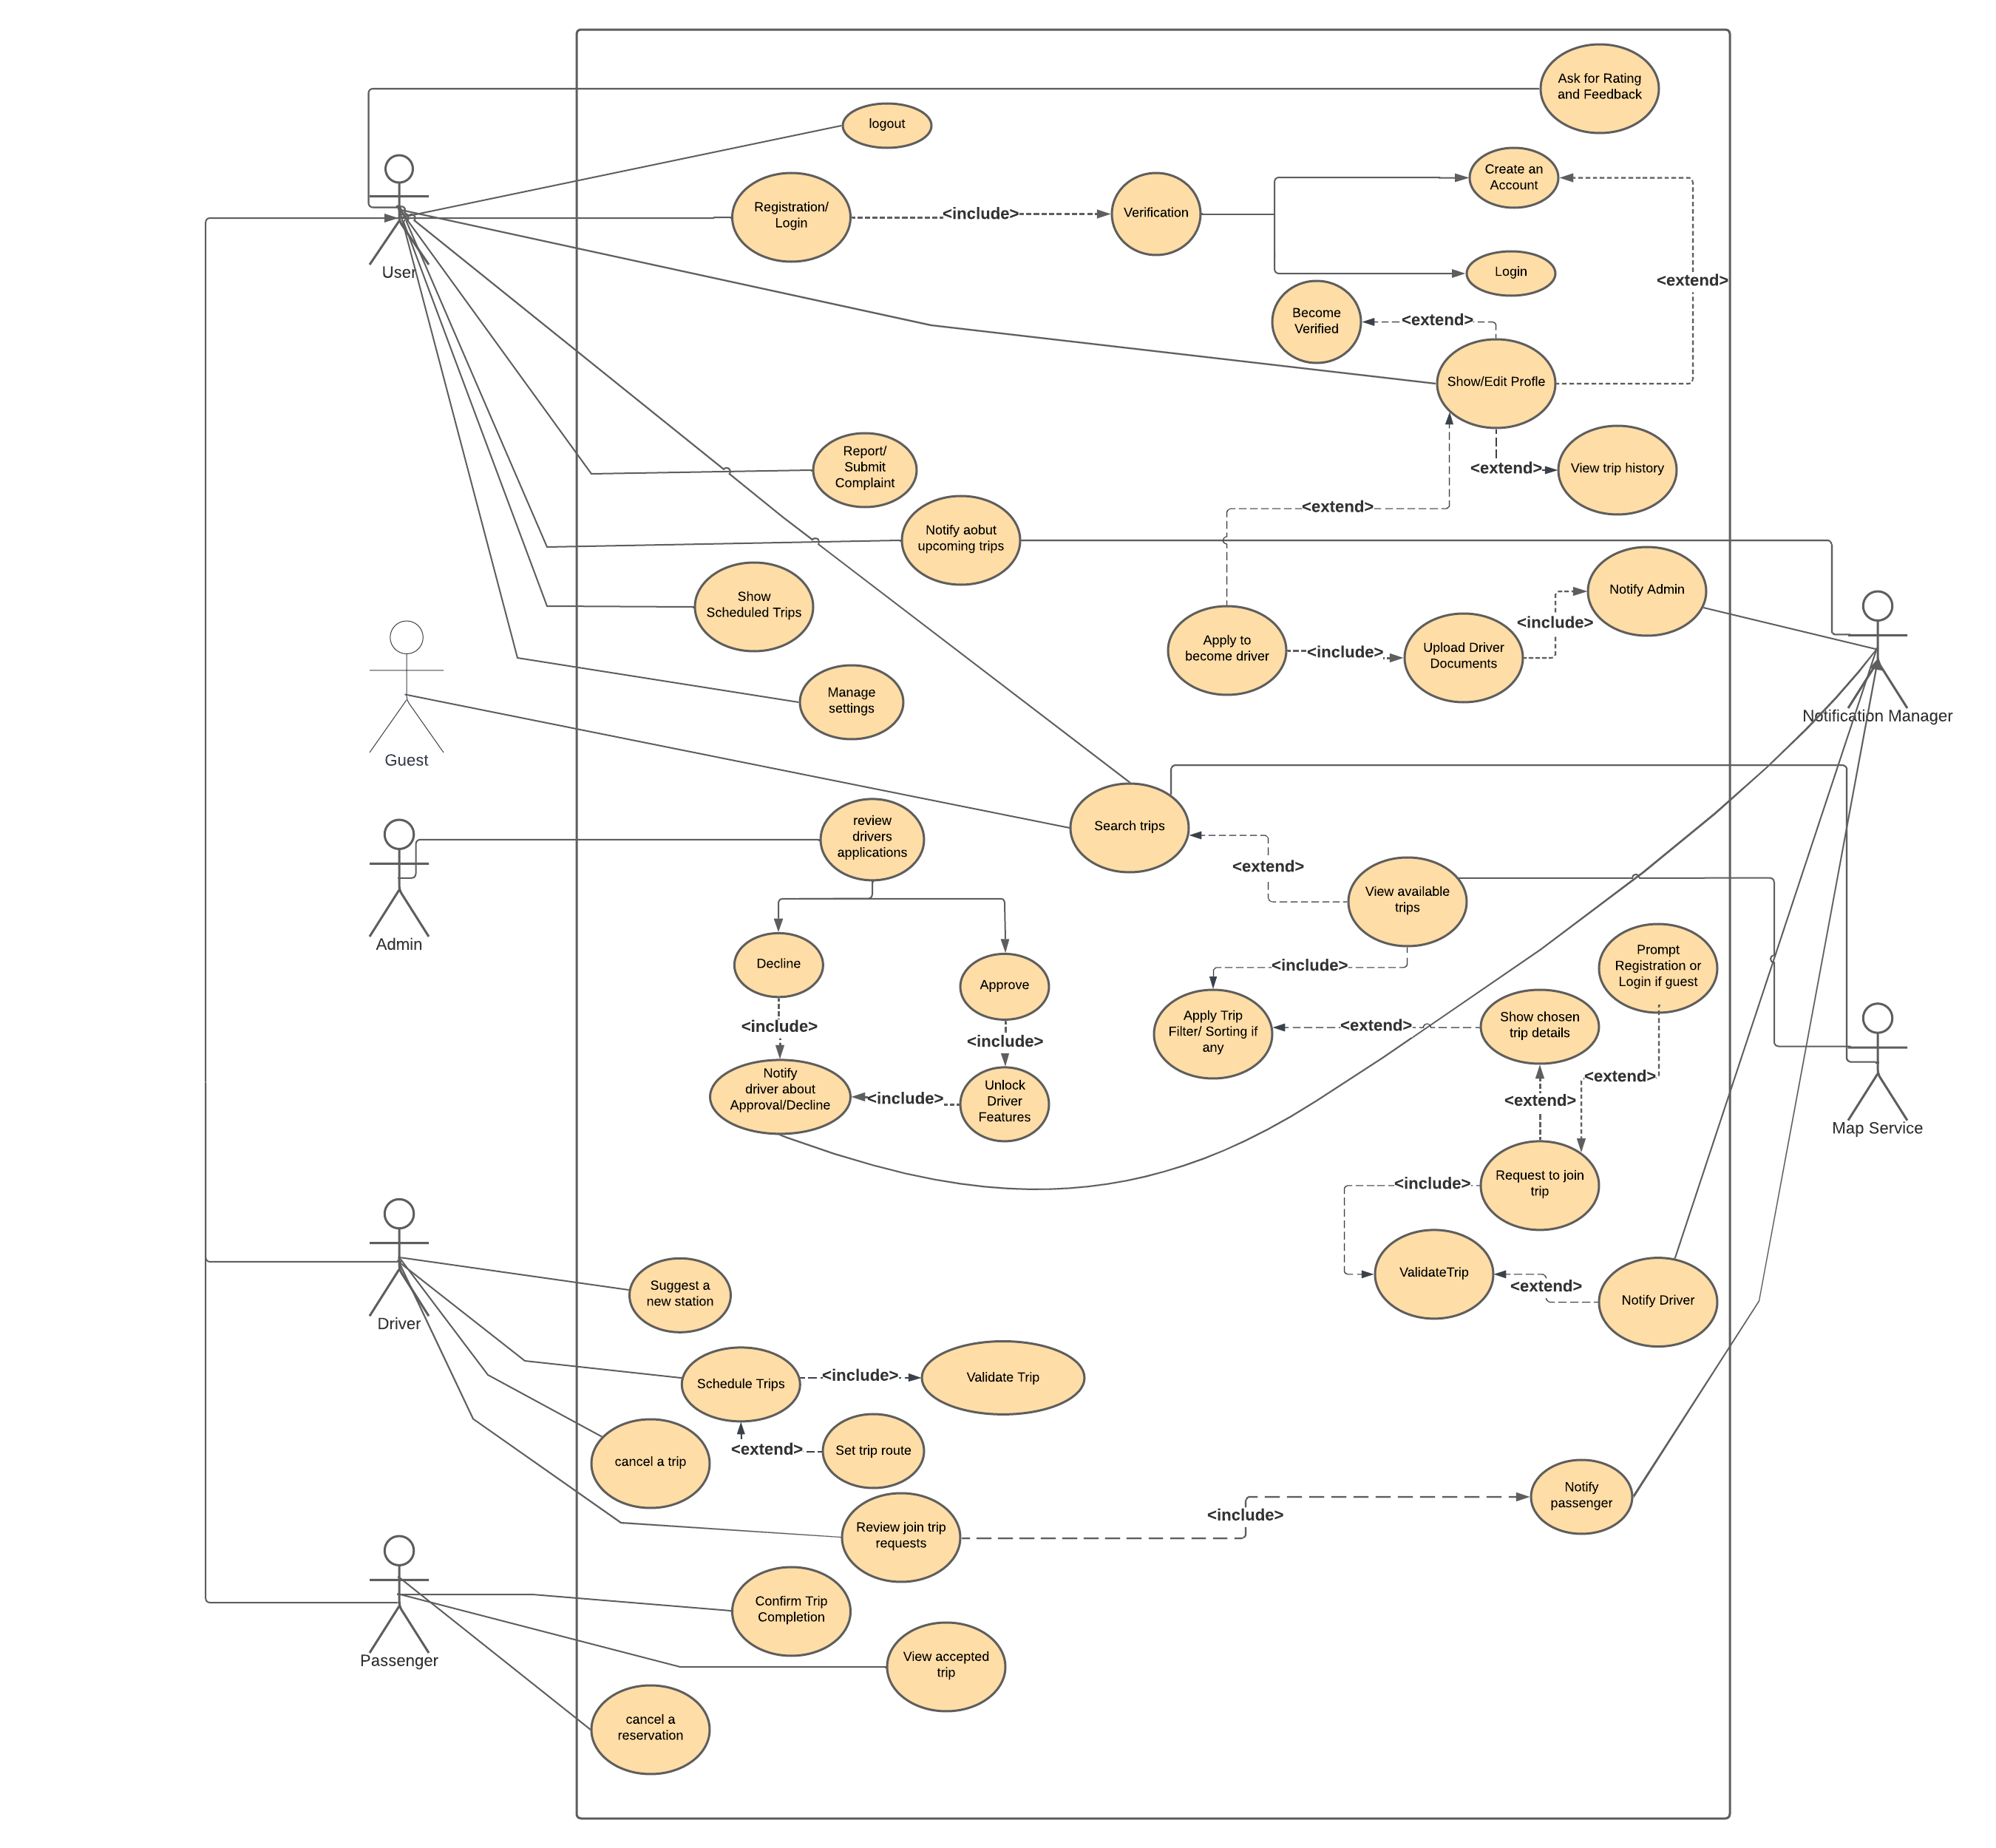
\includegraphics[width=1.2\textwidth]{Images/CarPal_Usecase.png}}
                \caption{Use Case Diagram}
                \label{fig:usecase}
            \end{figure}

    \pagebreak
    \subsection{Sequence, UML, State, and Deployment Diagrams}

        \begin{figure}[H]
            \centering
            \rotatebox{90}{
            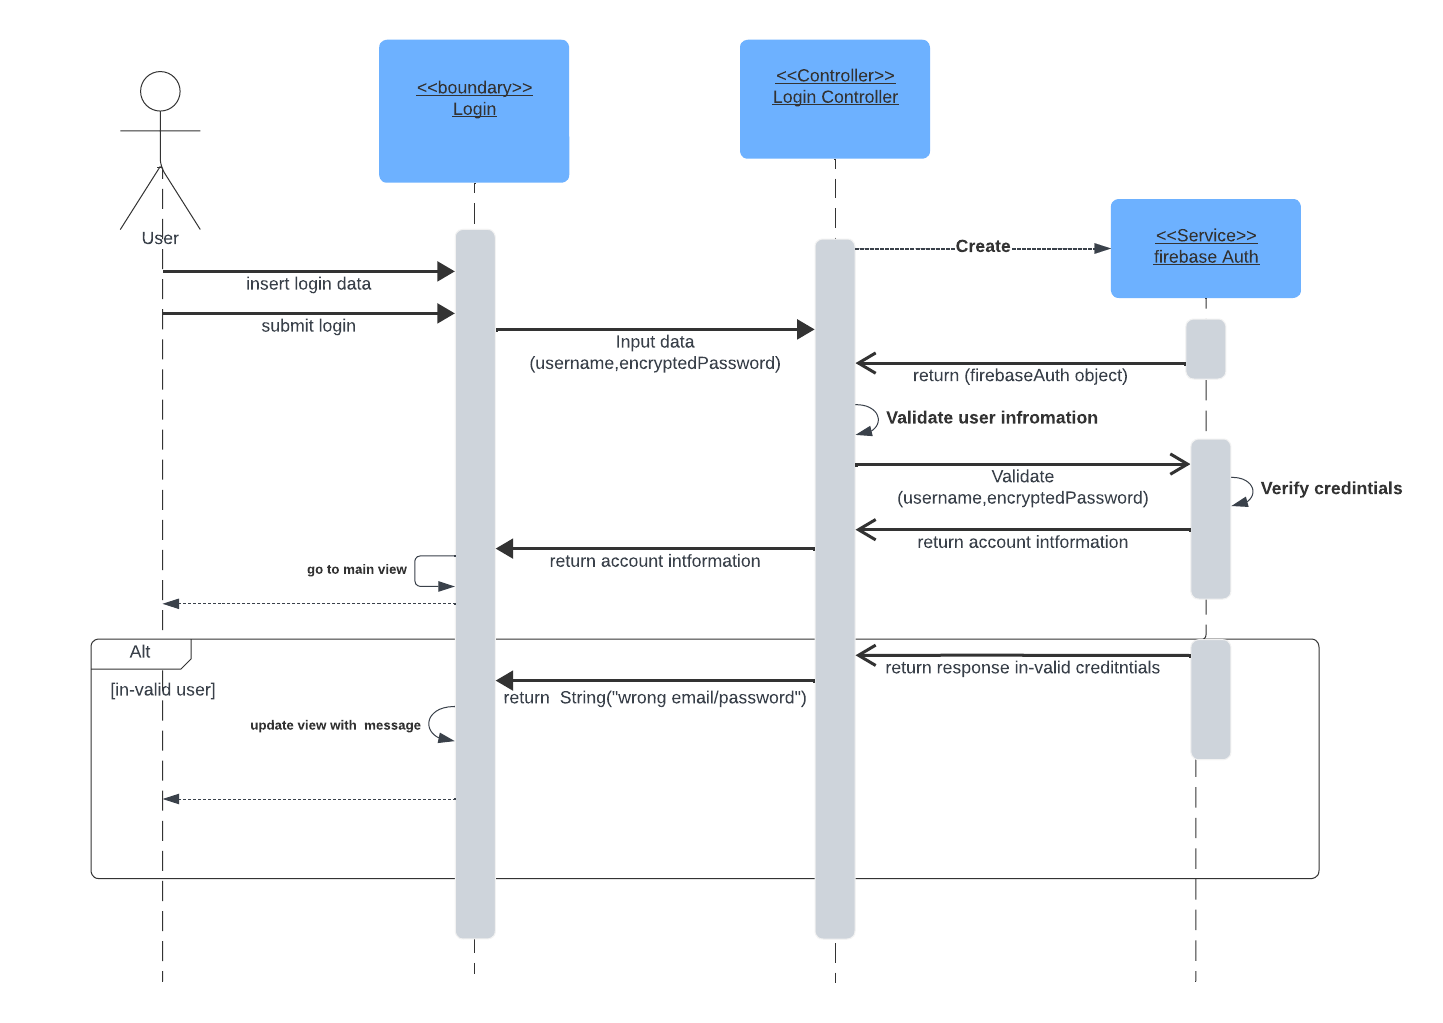
\includegraphics[width=1.1\textwidth]{Images/login.png}}
            \caption{Login Workflow}
            \label{fig:seq_dig_login}
        \end{figure}


    % \subsubsection{Login Sequence Diagram}
        % \begin{sidewaysfigure}
        %     \centering
        %     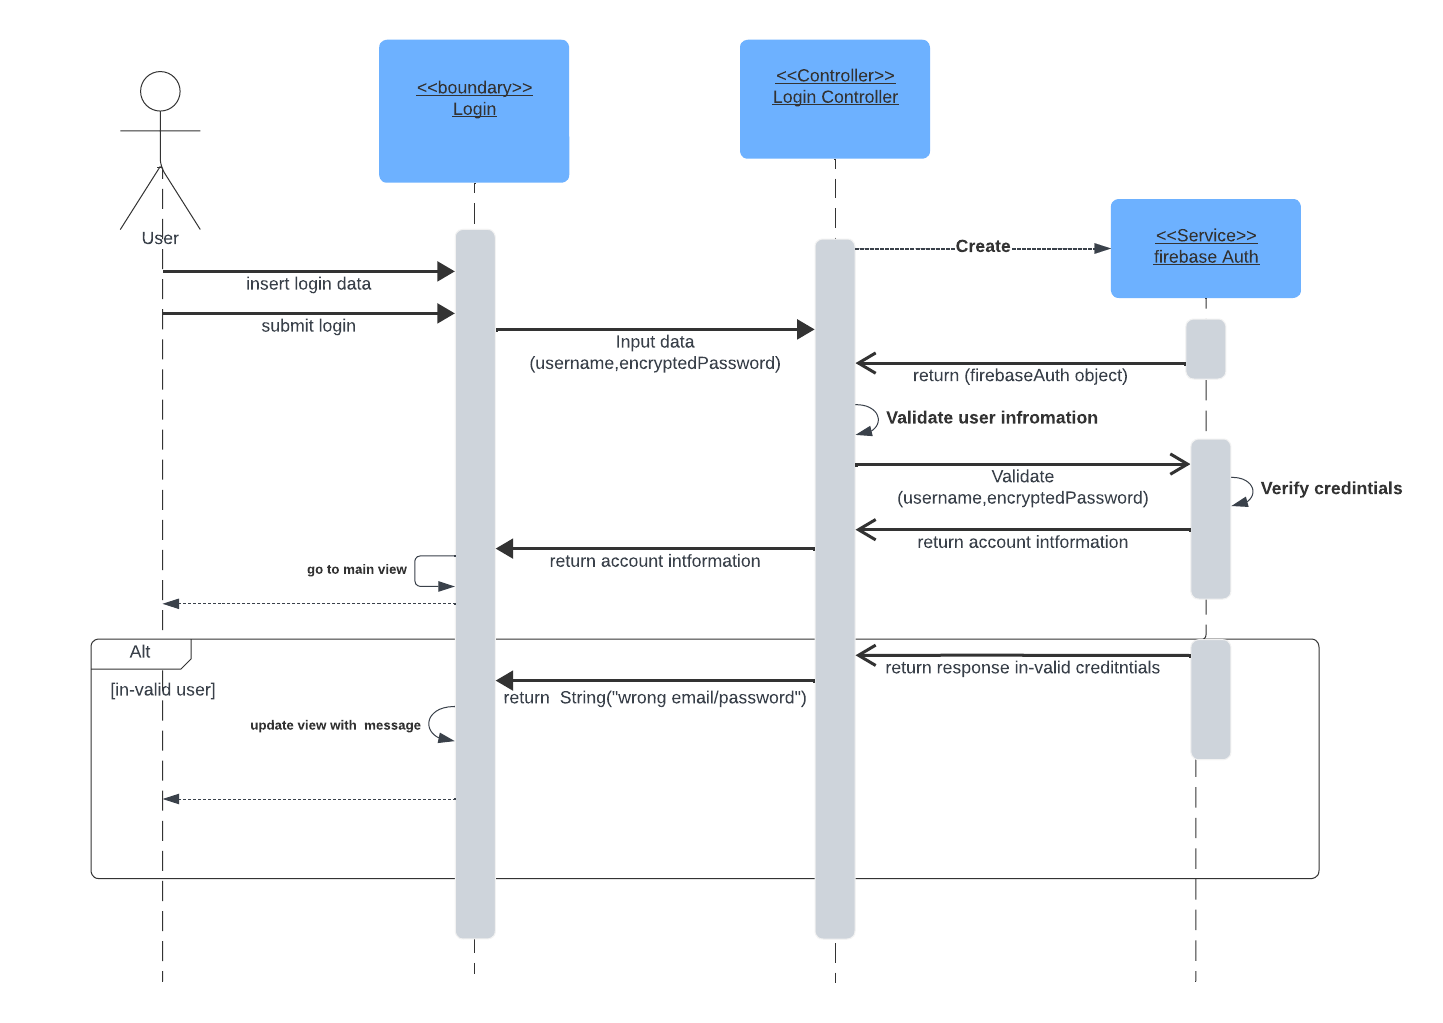
\includegraphics[width=\linewidth]{Images/login.png}
        %     \caption{Login Workflow}
        %     \label{fig:seq_dig_login}
        % \end{sidewaysfigure}
    % \subsubsection{Accepted trips Sequence Diagram}       
    
        \begin{sidewaysfigure}[!htb]
            \centering
            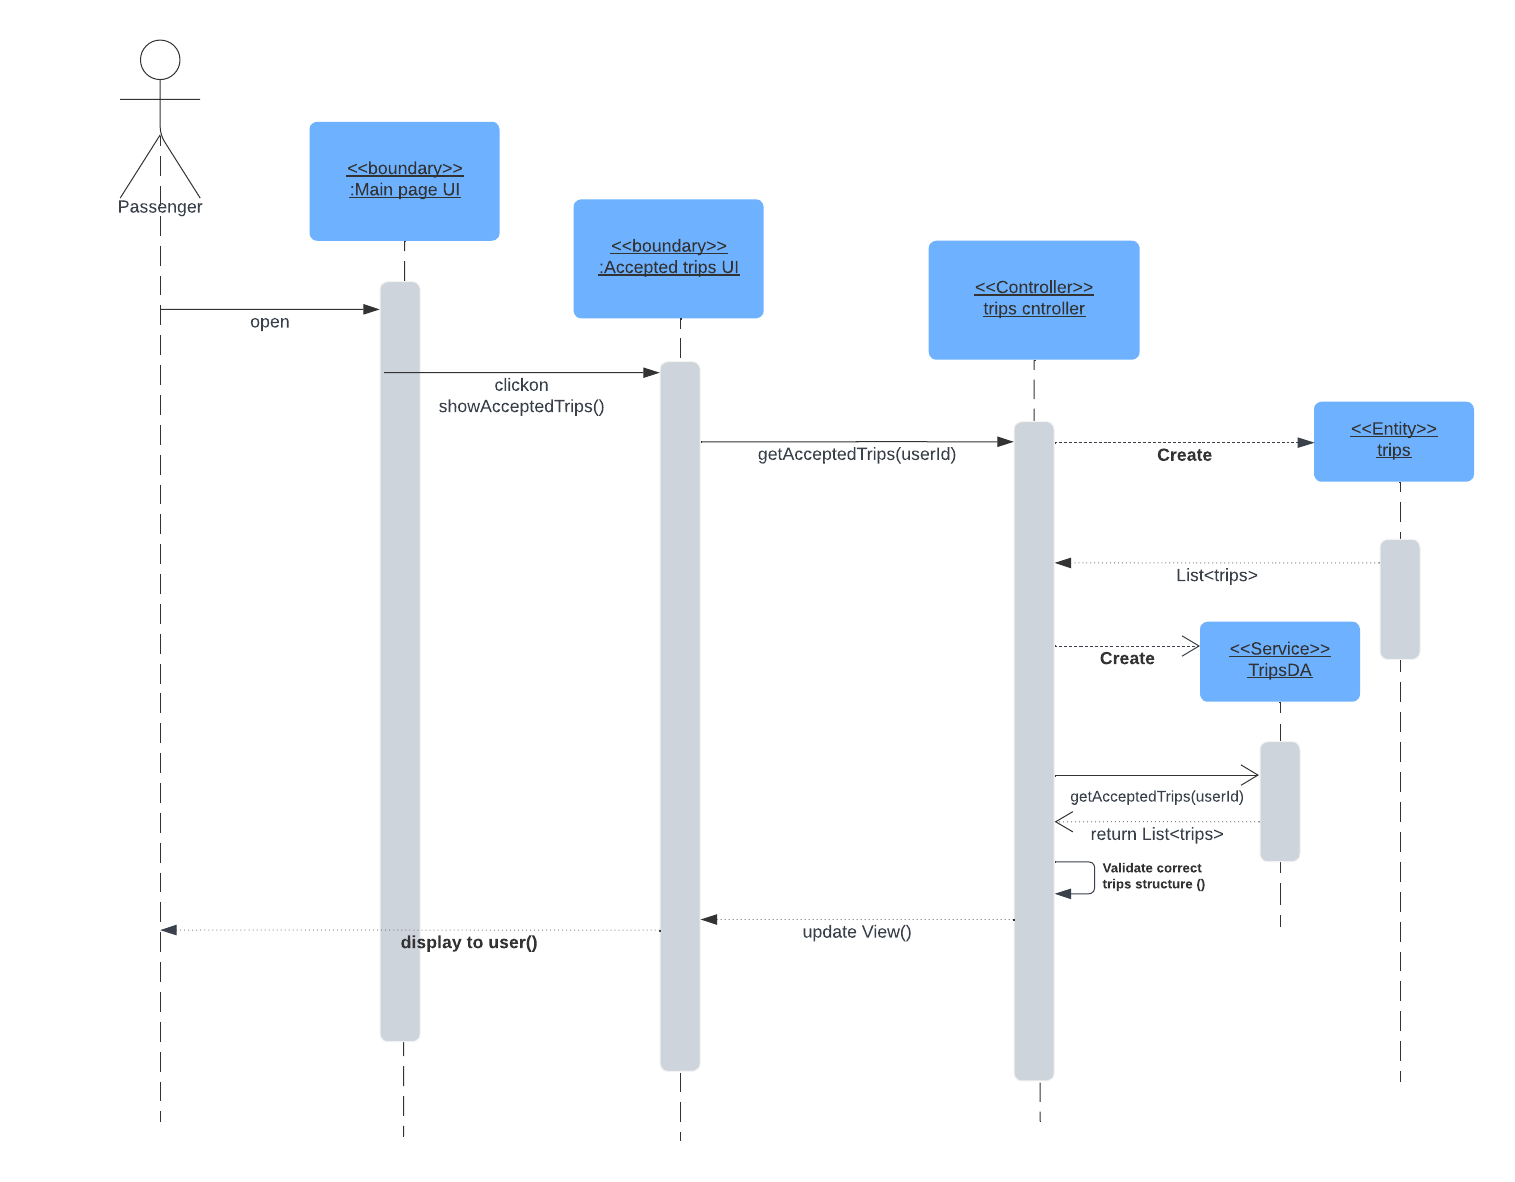
\includegraphics[width=0.9\linewidth]{Images/Passenger Accepted.png}
            \caption{Showing Passenger's Accepted Trips Action}
            \label{fig:seq_dig_pass_accepted}
        \end{sidewaysfigure}

        \FloatBarrier


    % \subsubsection{Reserve Seat sequence Diagram}
        \begin{sidewaysfigure}[!htb]
            \centering
            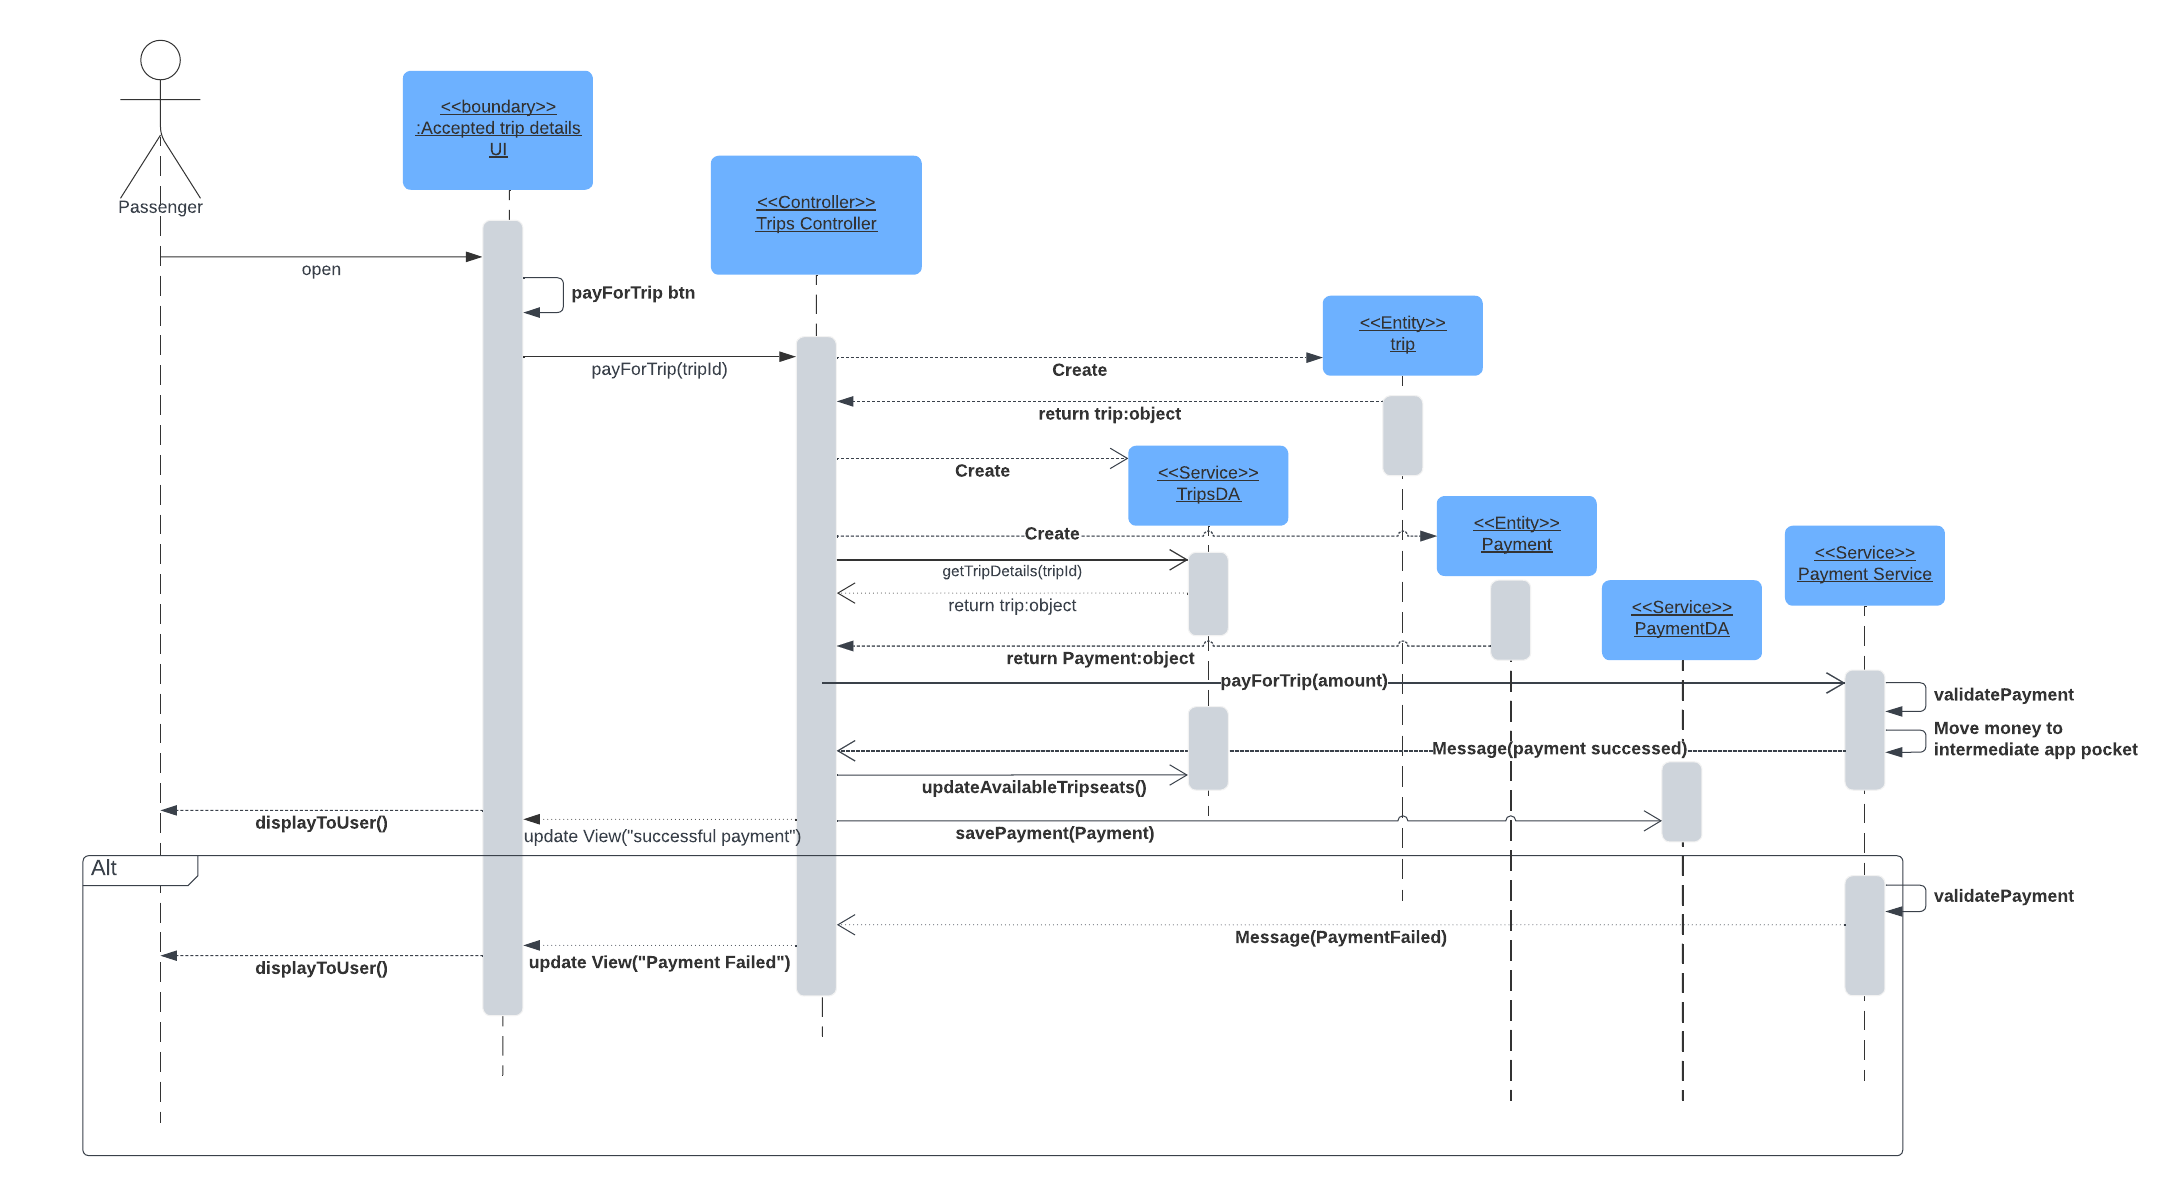
\includegraphics[width=\linewidth]{Images/Passenger Payment.png}
            \caption{Passenger Payment Workflow}
            \label{fig:seq_dig_pass_payment}
        \end{sidewaysfigure}

        \FloatBarrier


    % \subsubsection{show scheduled trips sequence Diagram}
        \begin{sidewaysfigure}[!htb]
            \centering
            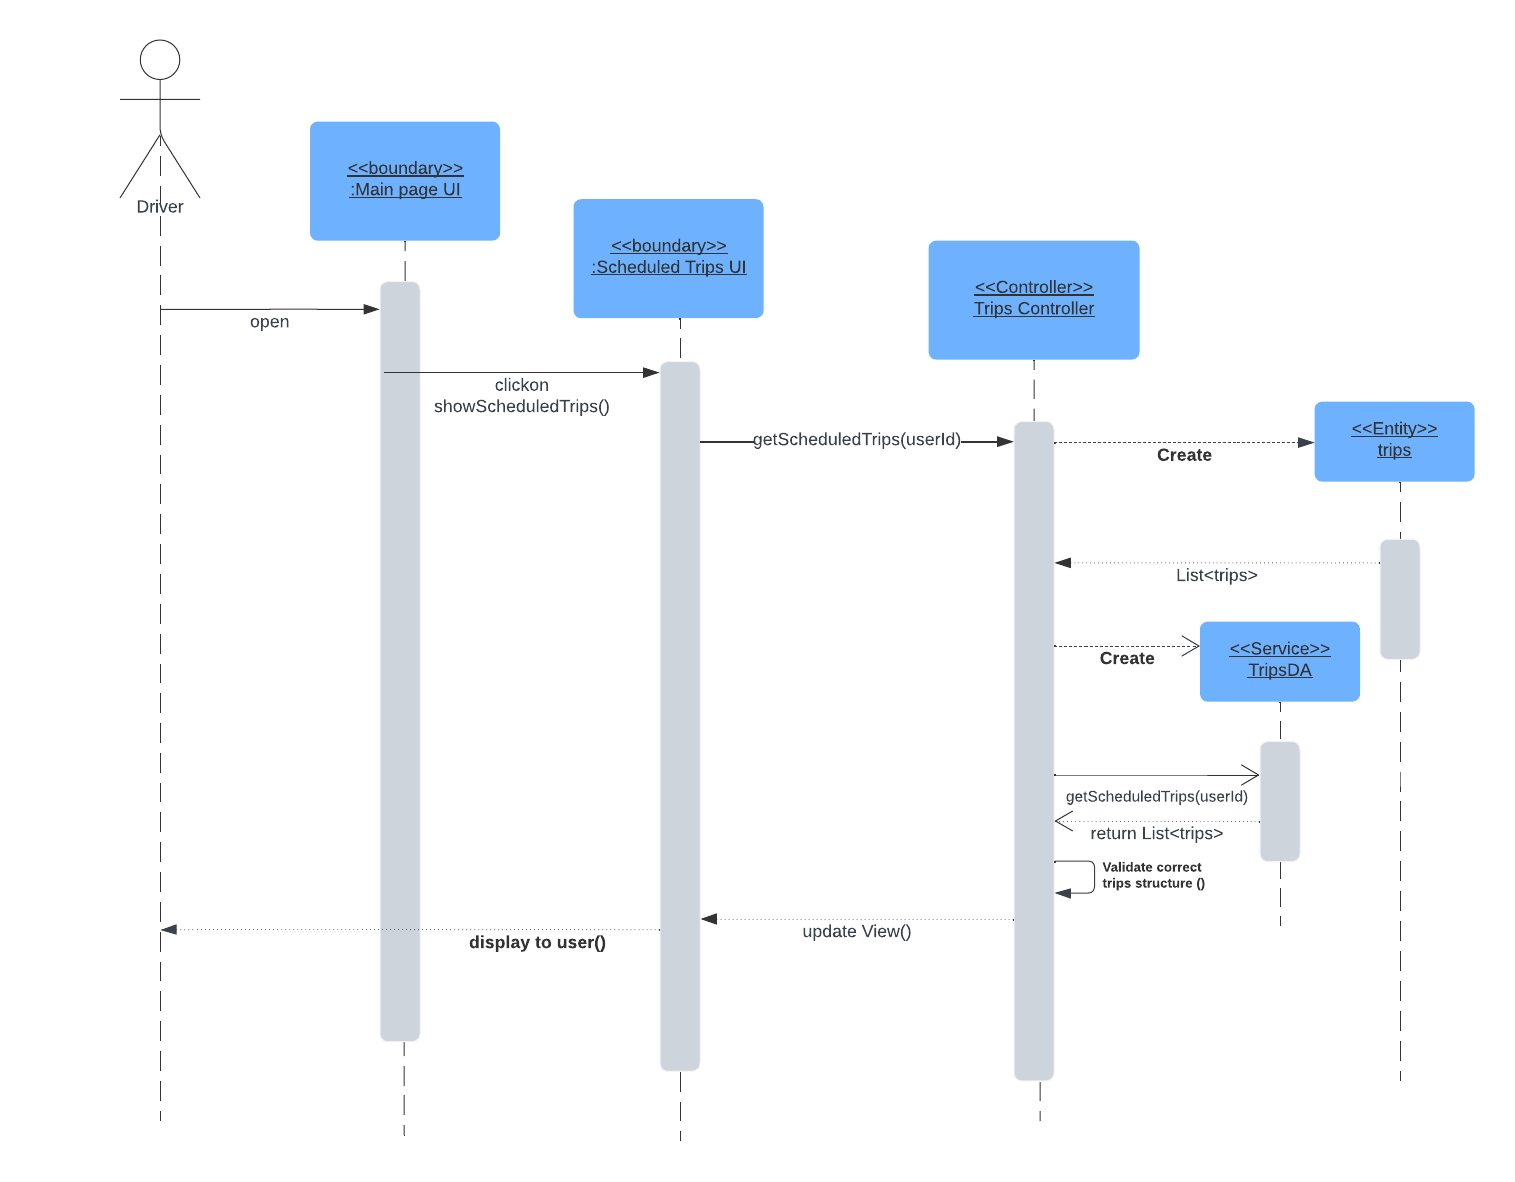
\includegraphics[width=\linewidth]{Images/Driver Scheduled.png}
            \caption{Showing Driver's Scheduled Trips Action}
            \label{fig:seq_dig_driver_scheduled}
        \end{sidewaysfigure}

        \FloatBarrier

    % \subsubsection{Driver Accepts trip Request sequence Diagram}
        \begin{sidewaysfigure}[!htb]
            \centering
            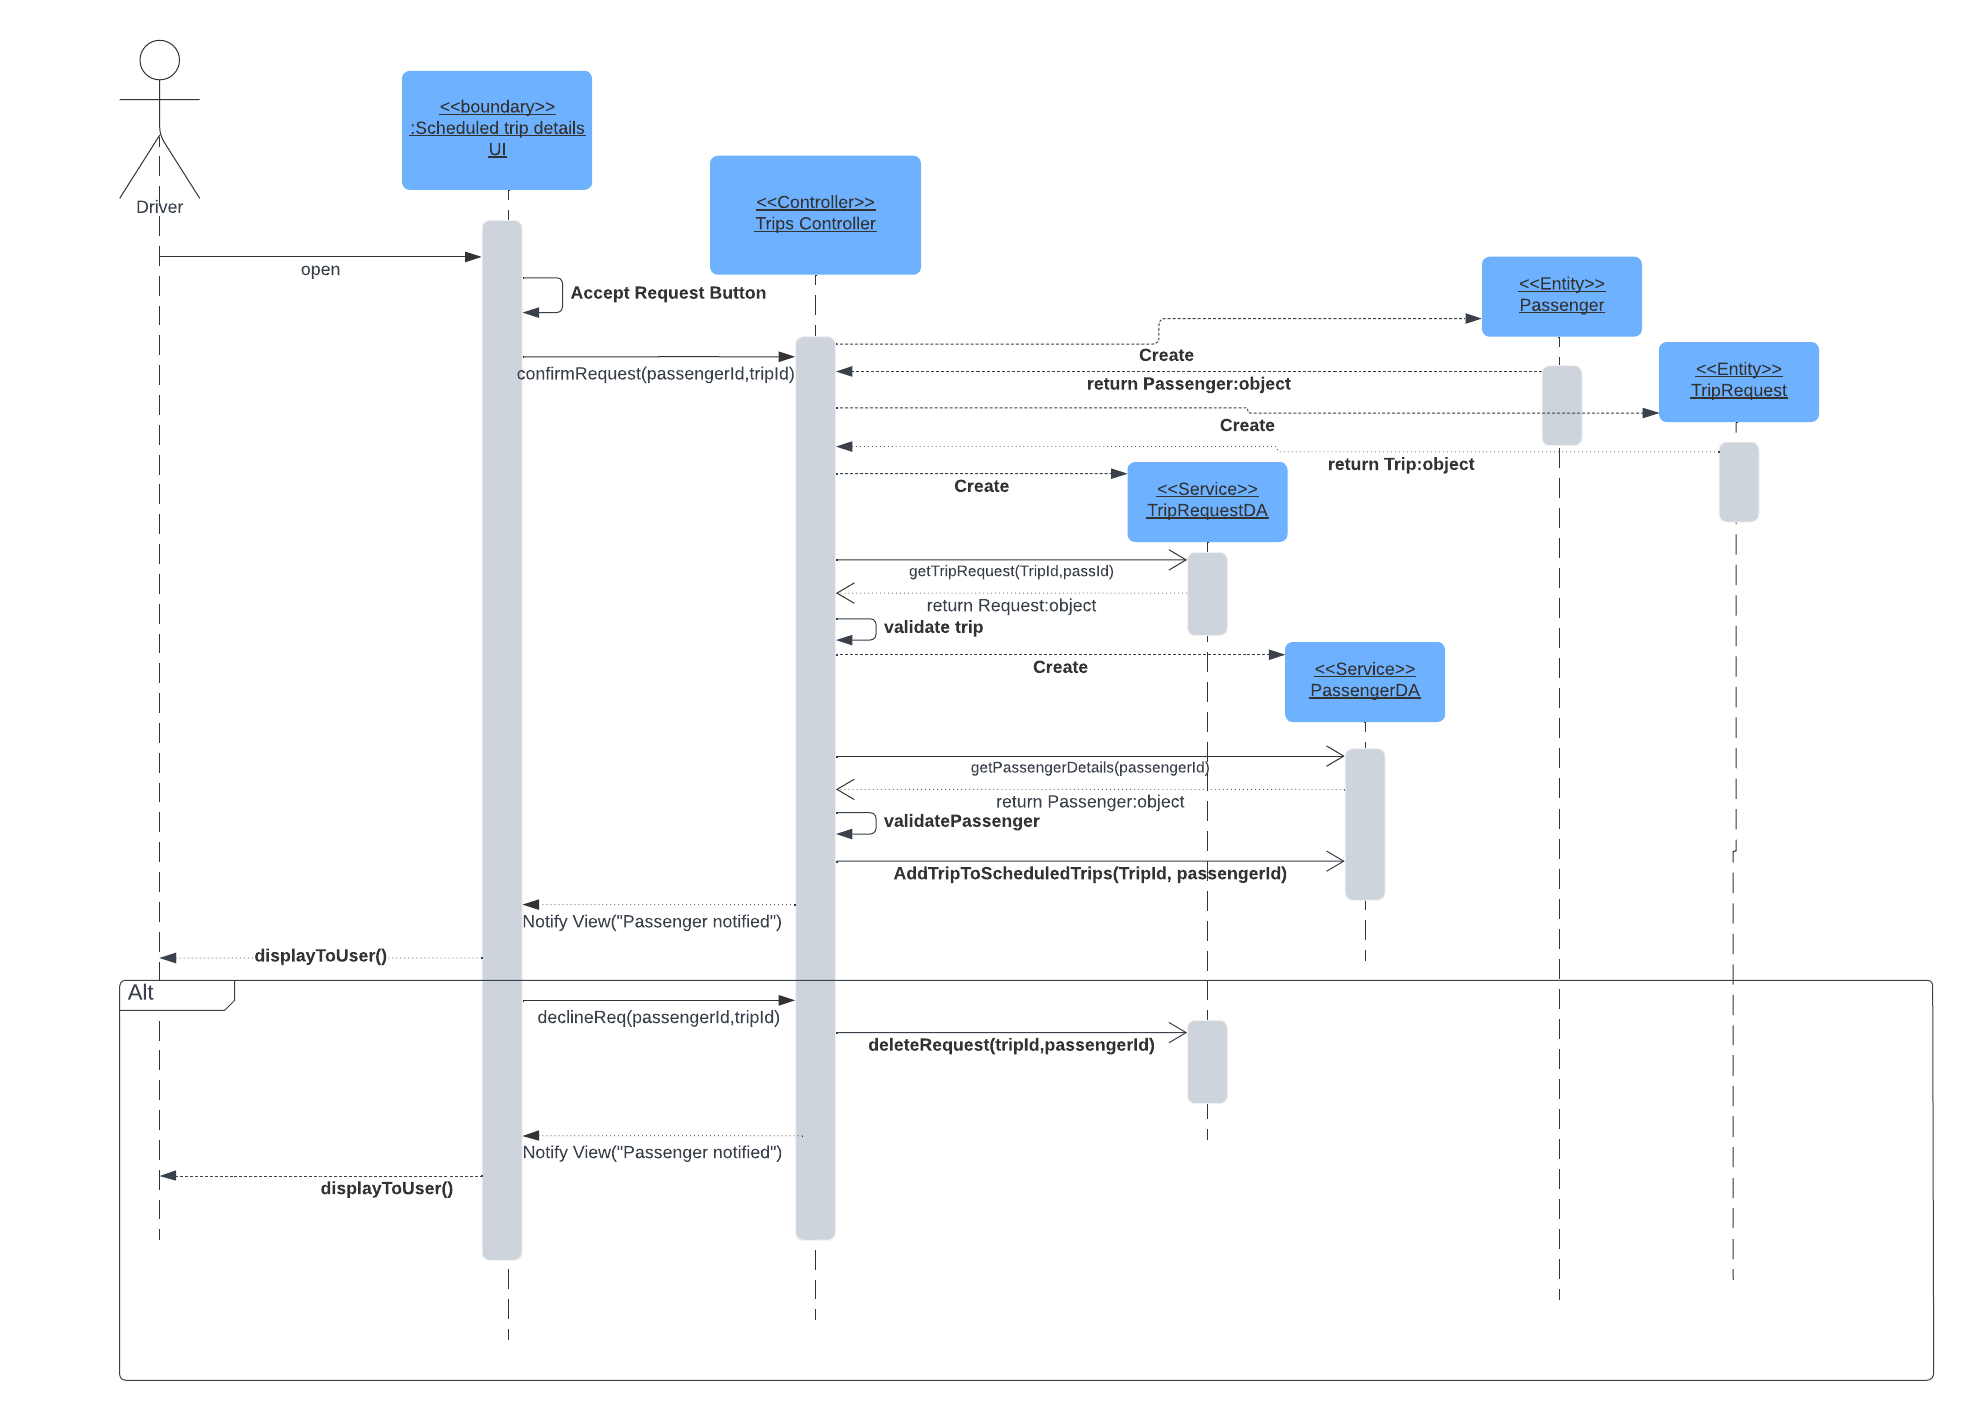
\includegraphics[width=\linewidth]{Images/Driver Request.png}
            \caption{Passenger Request Workflow}
            \label{fig:seq_dig_driver_request}
        \end{sidewaysfigure}

        \FloatBarrier

    % \subsubsection{UML Class Diagram}
        \begin{sidewaysfigure}[!htb]
            \centering
            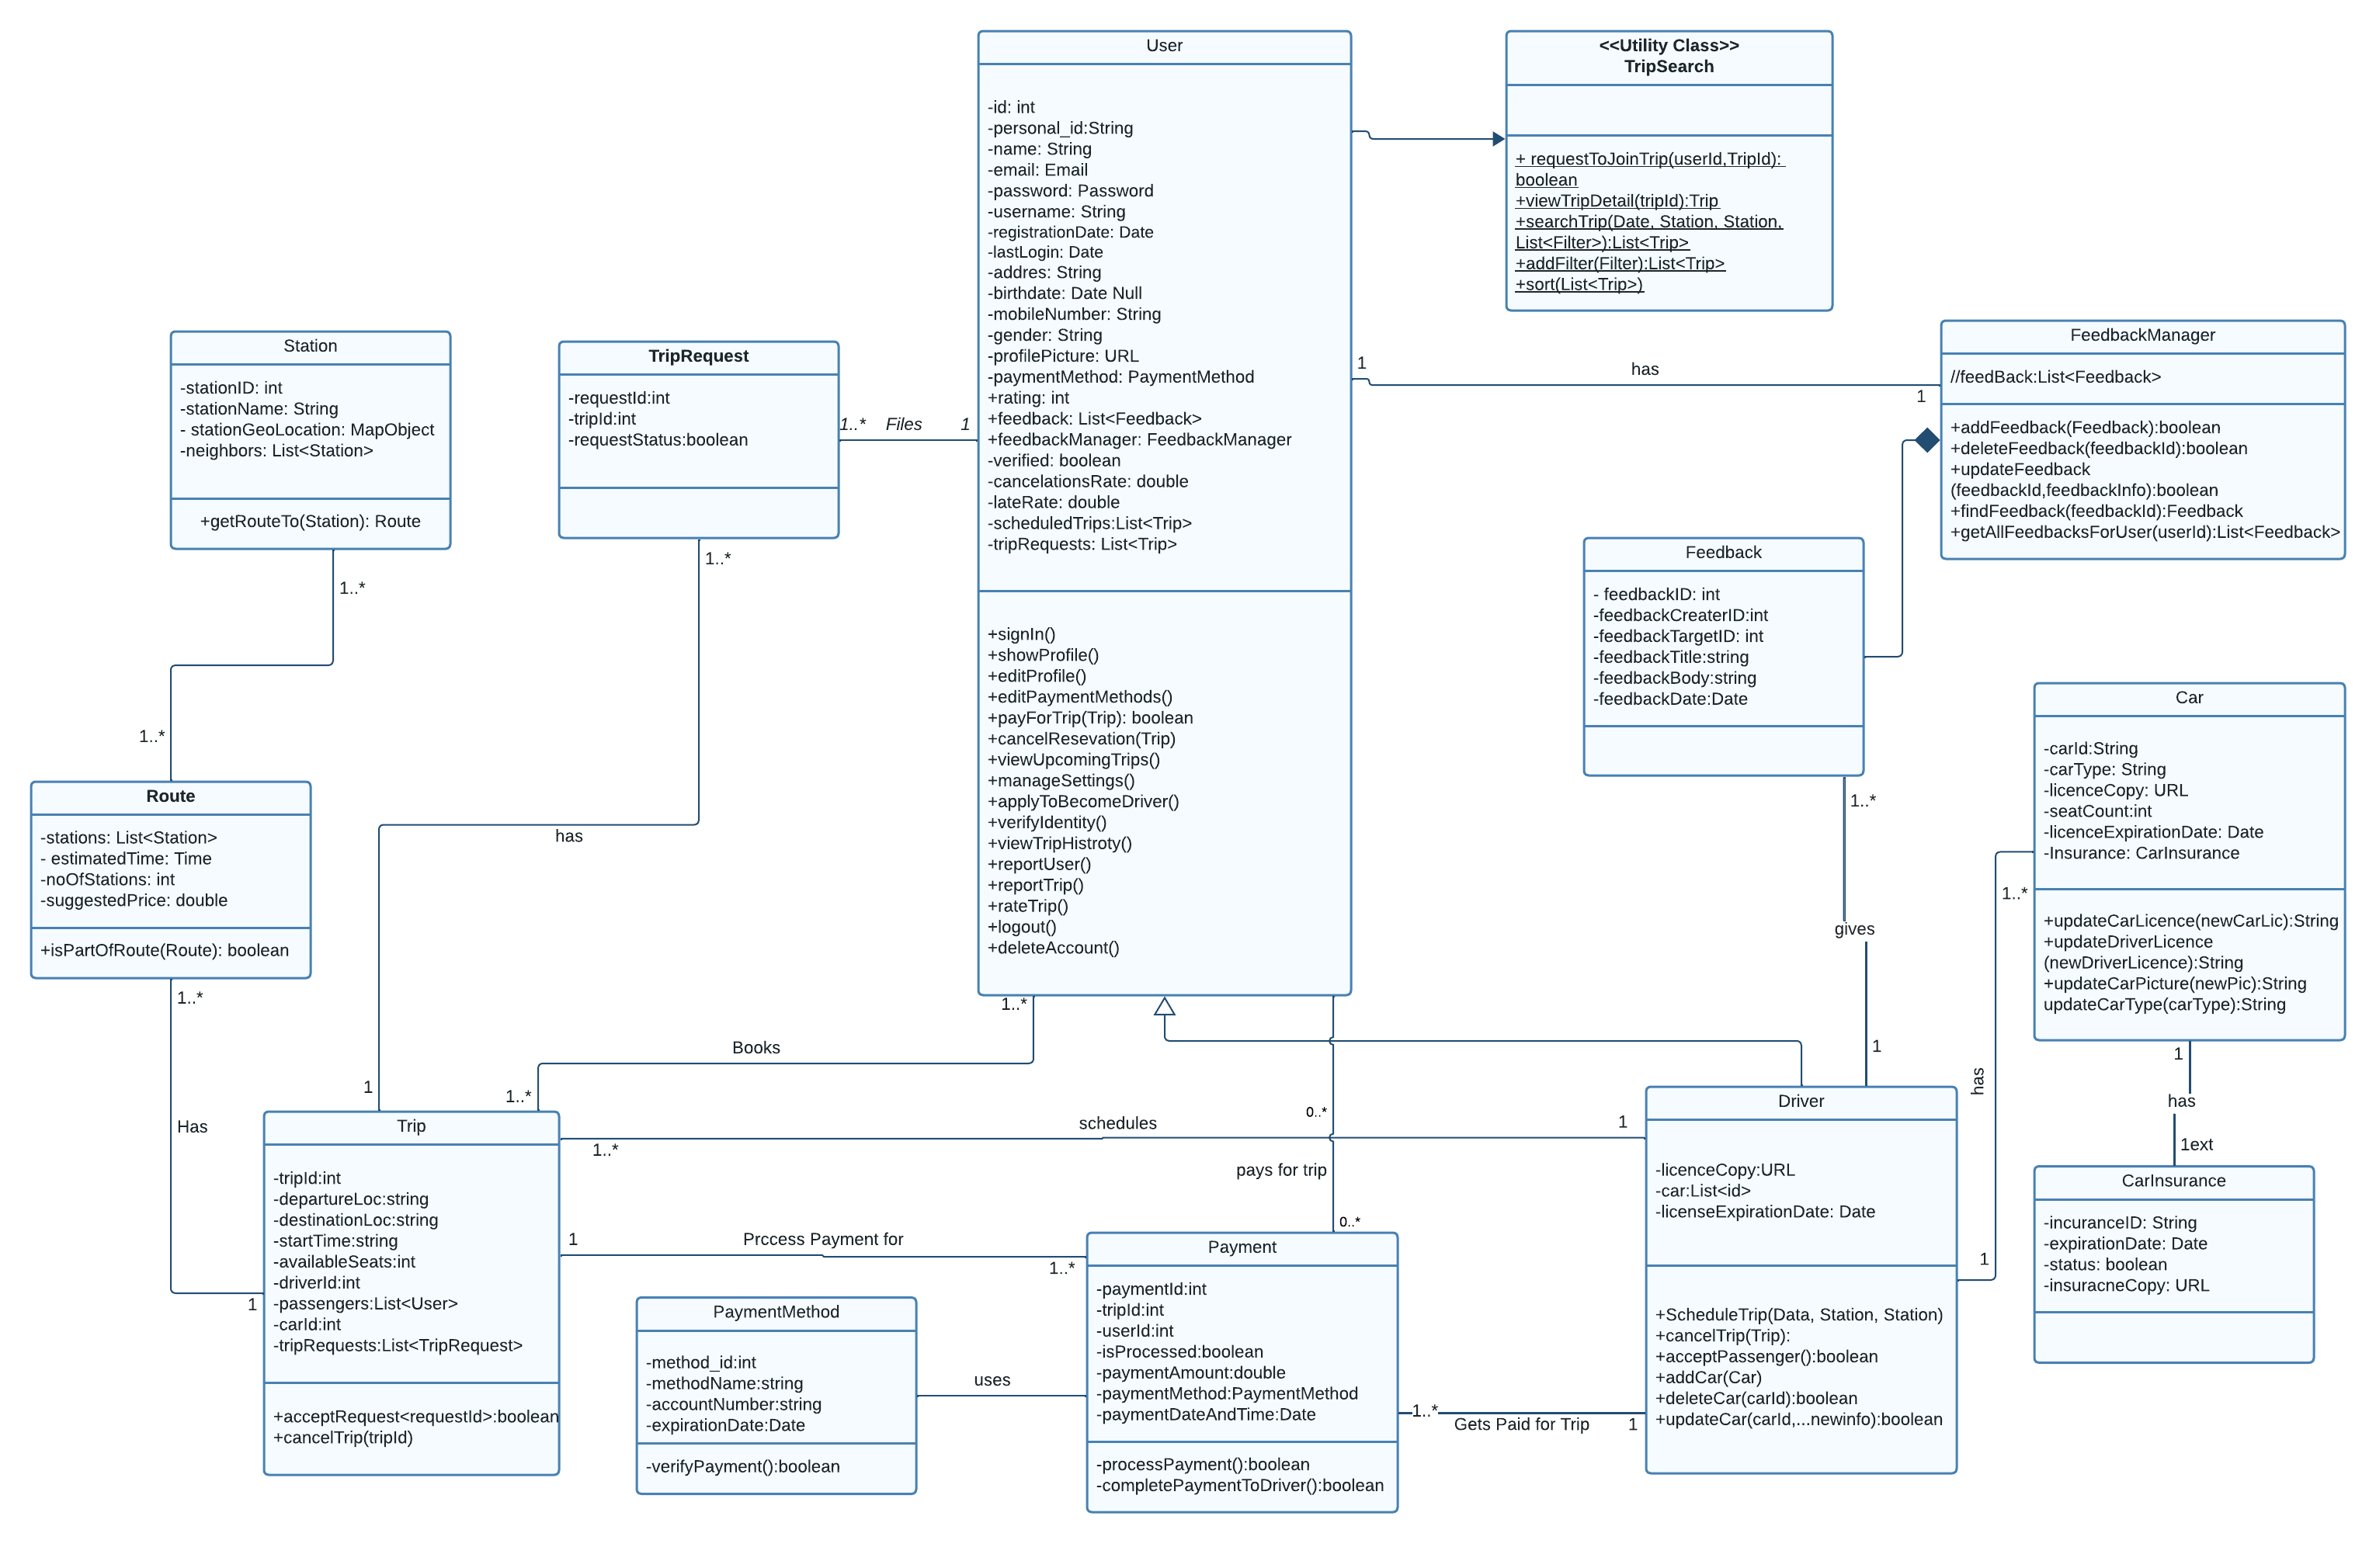
\includegraphics[width=\linewidth]{Images/UML Class.png}
            \caption{UML Class Diagram}
            \label{fig:class_diagram}
        \end{sidewaysfigure}

        \FloatBarrier
        
    % \subsubsection{State Diagrams}
        \begin{sidewaysfigure}[!htb]
            \centering
            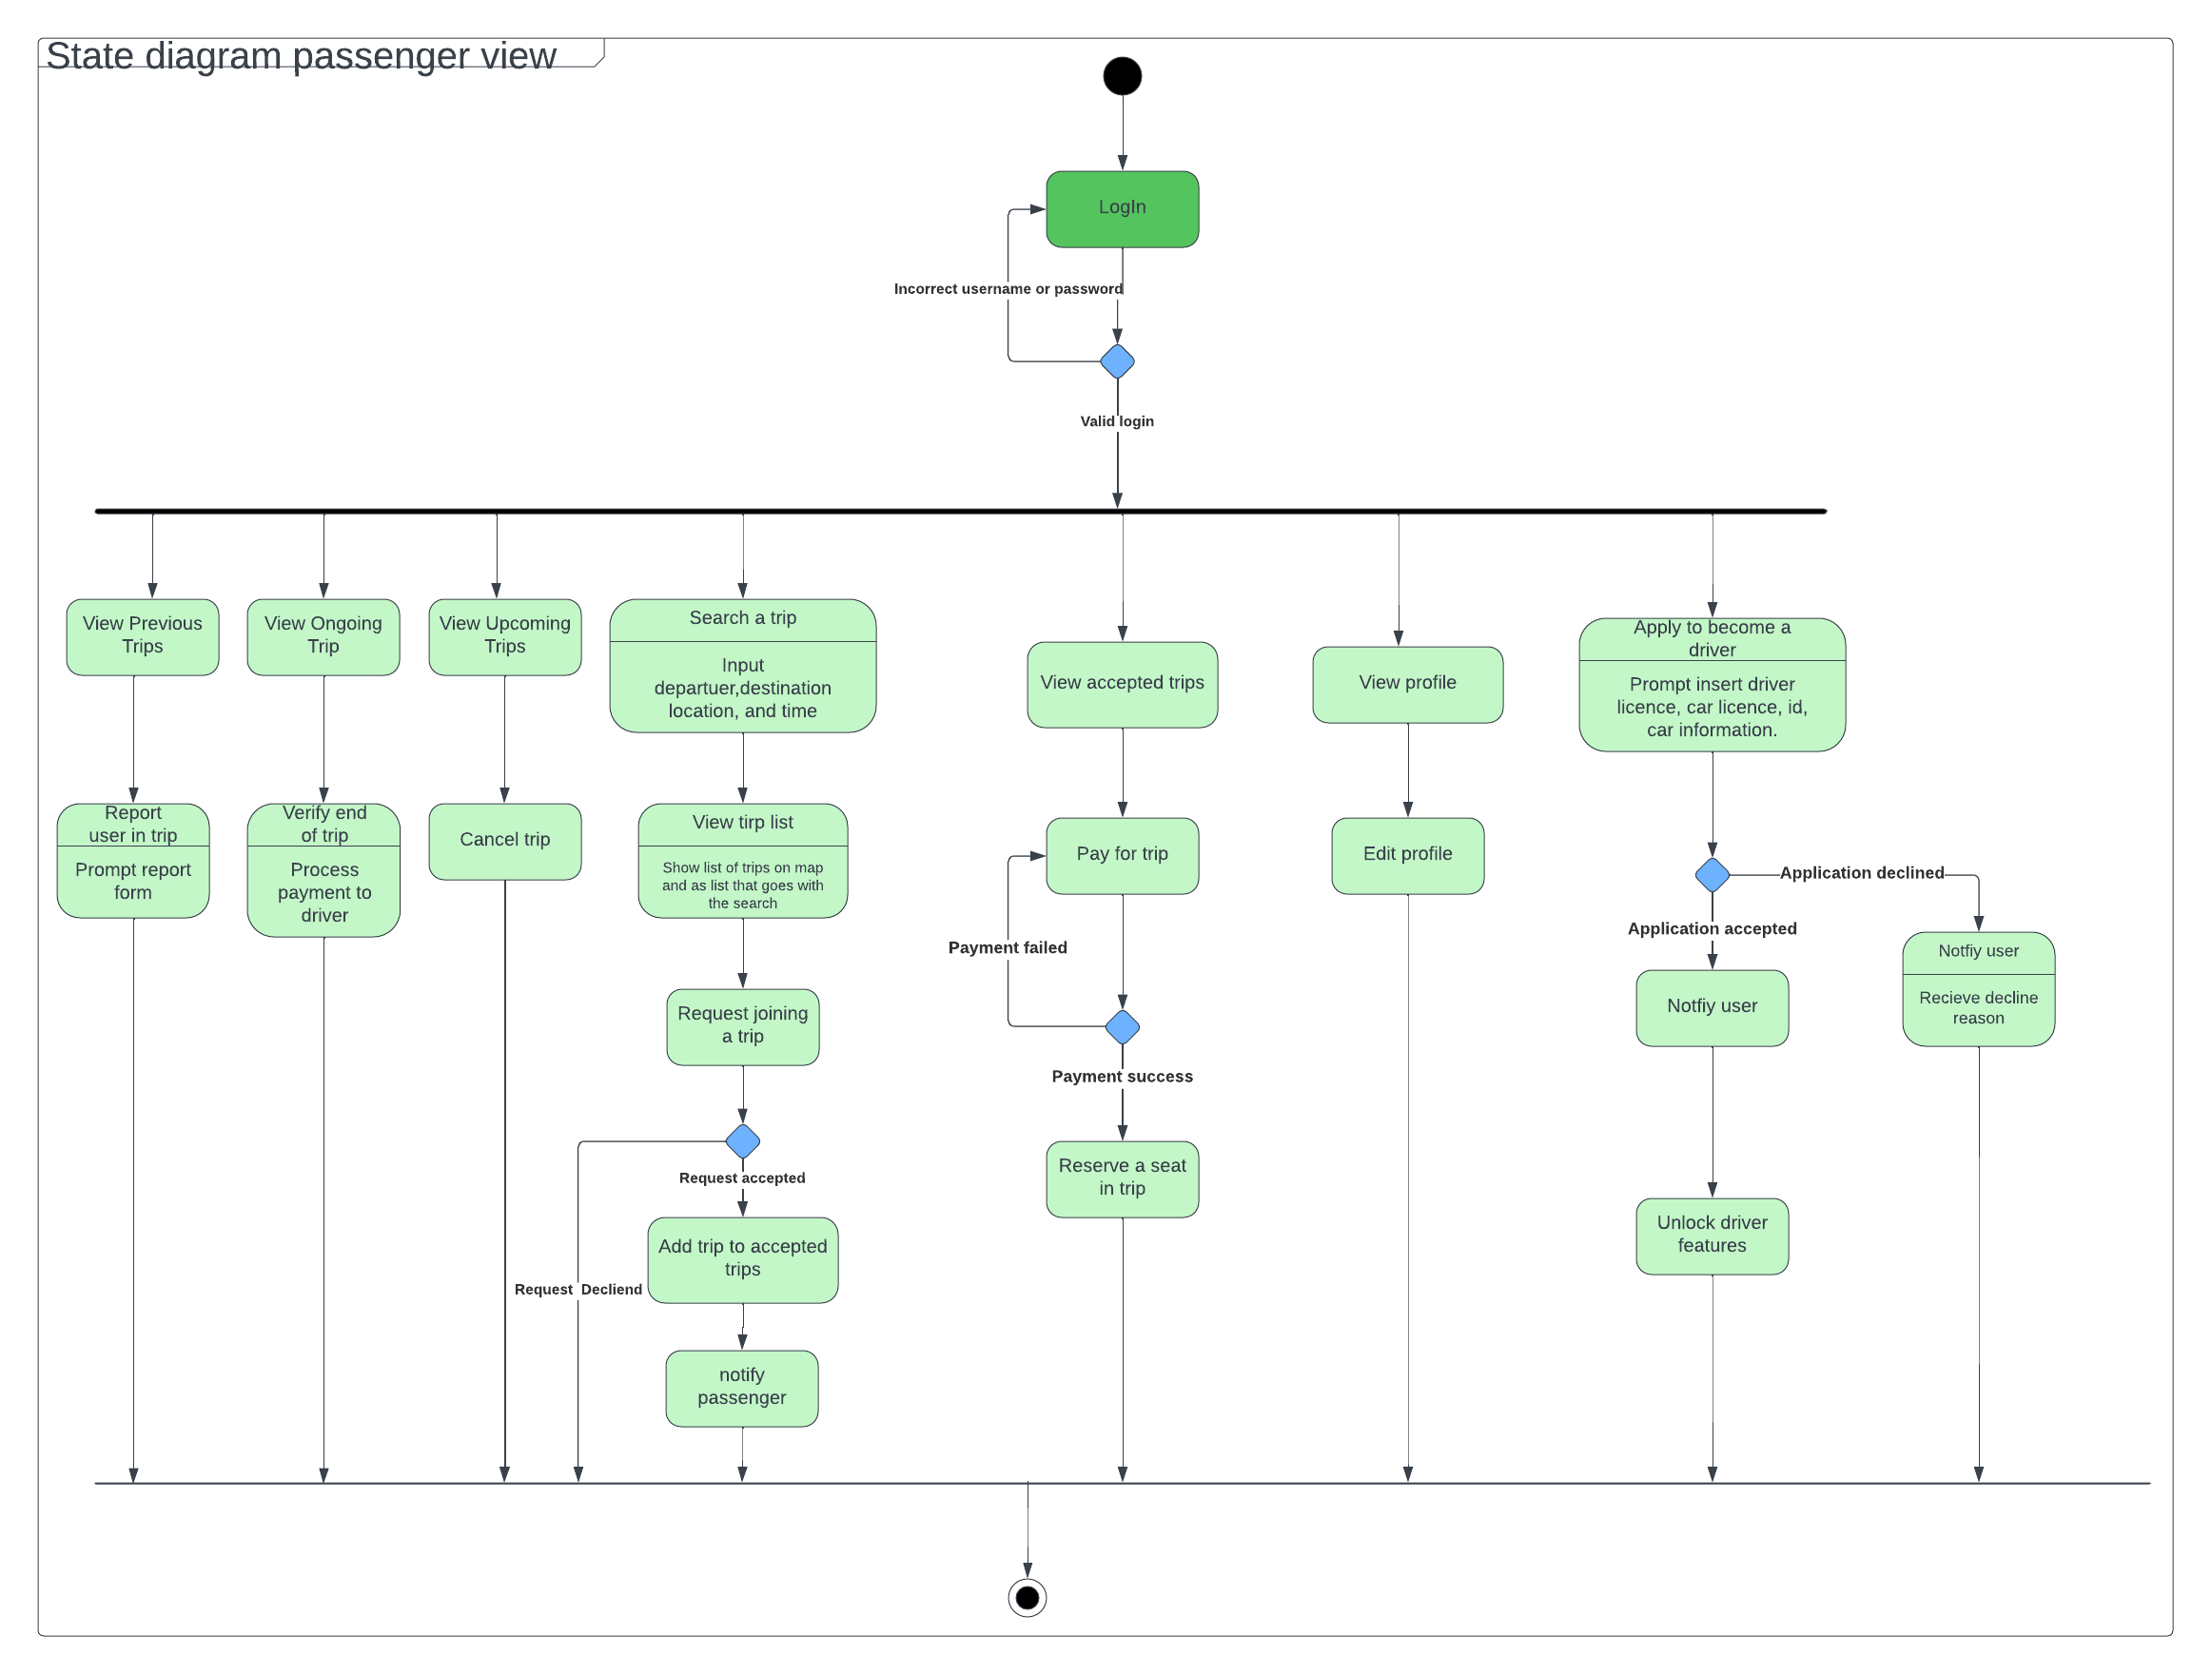
\includegraphics[width=\linewidth]{Images/State Diagram passenger.png}
            \caption{State Diagram for Passenger}
            \label{fig:state_passenger}
        \end{sidewaysfigure}

        \FloatBarrier

       \begin{sidewaysfigure}[!htb]
            \centering
            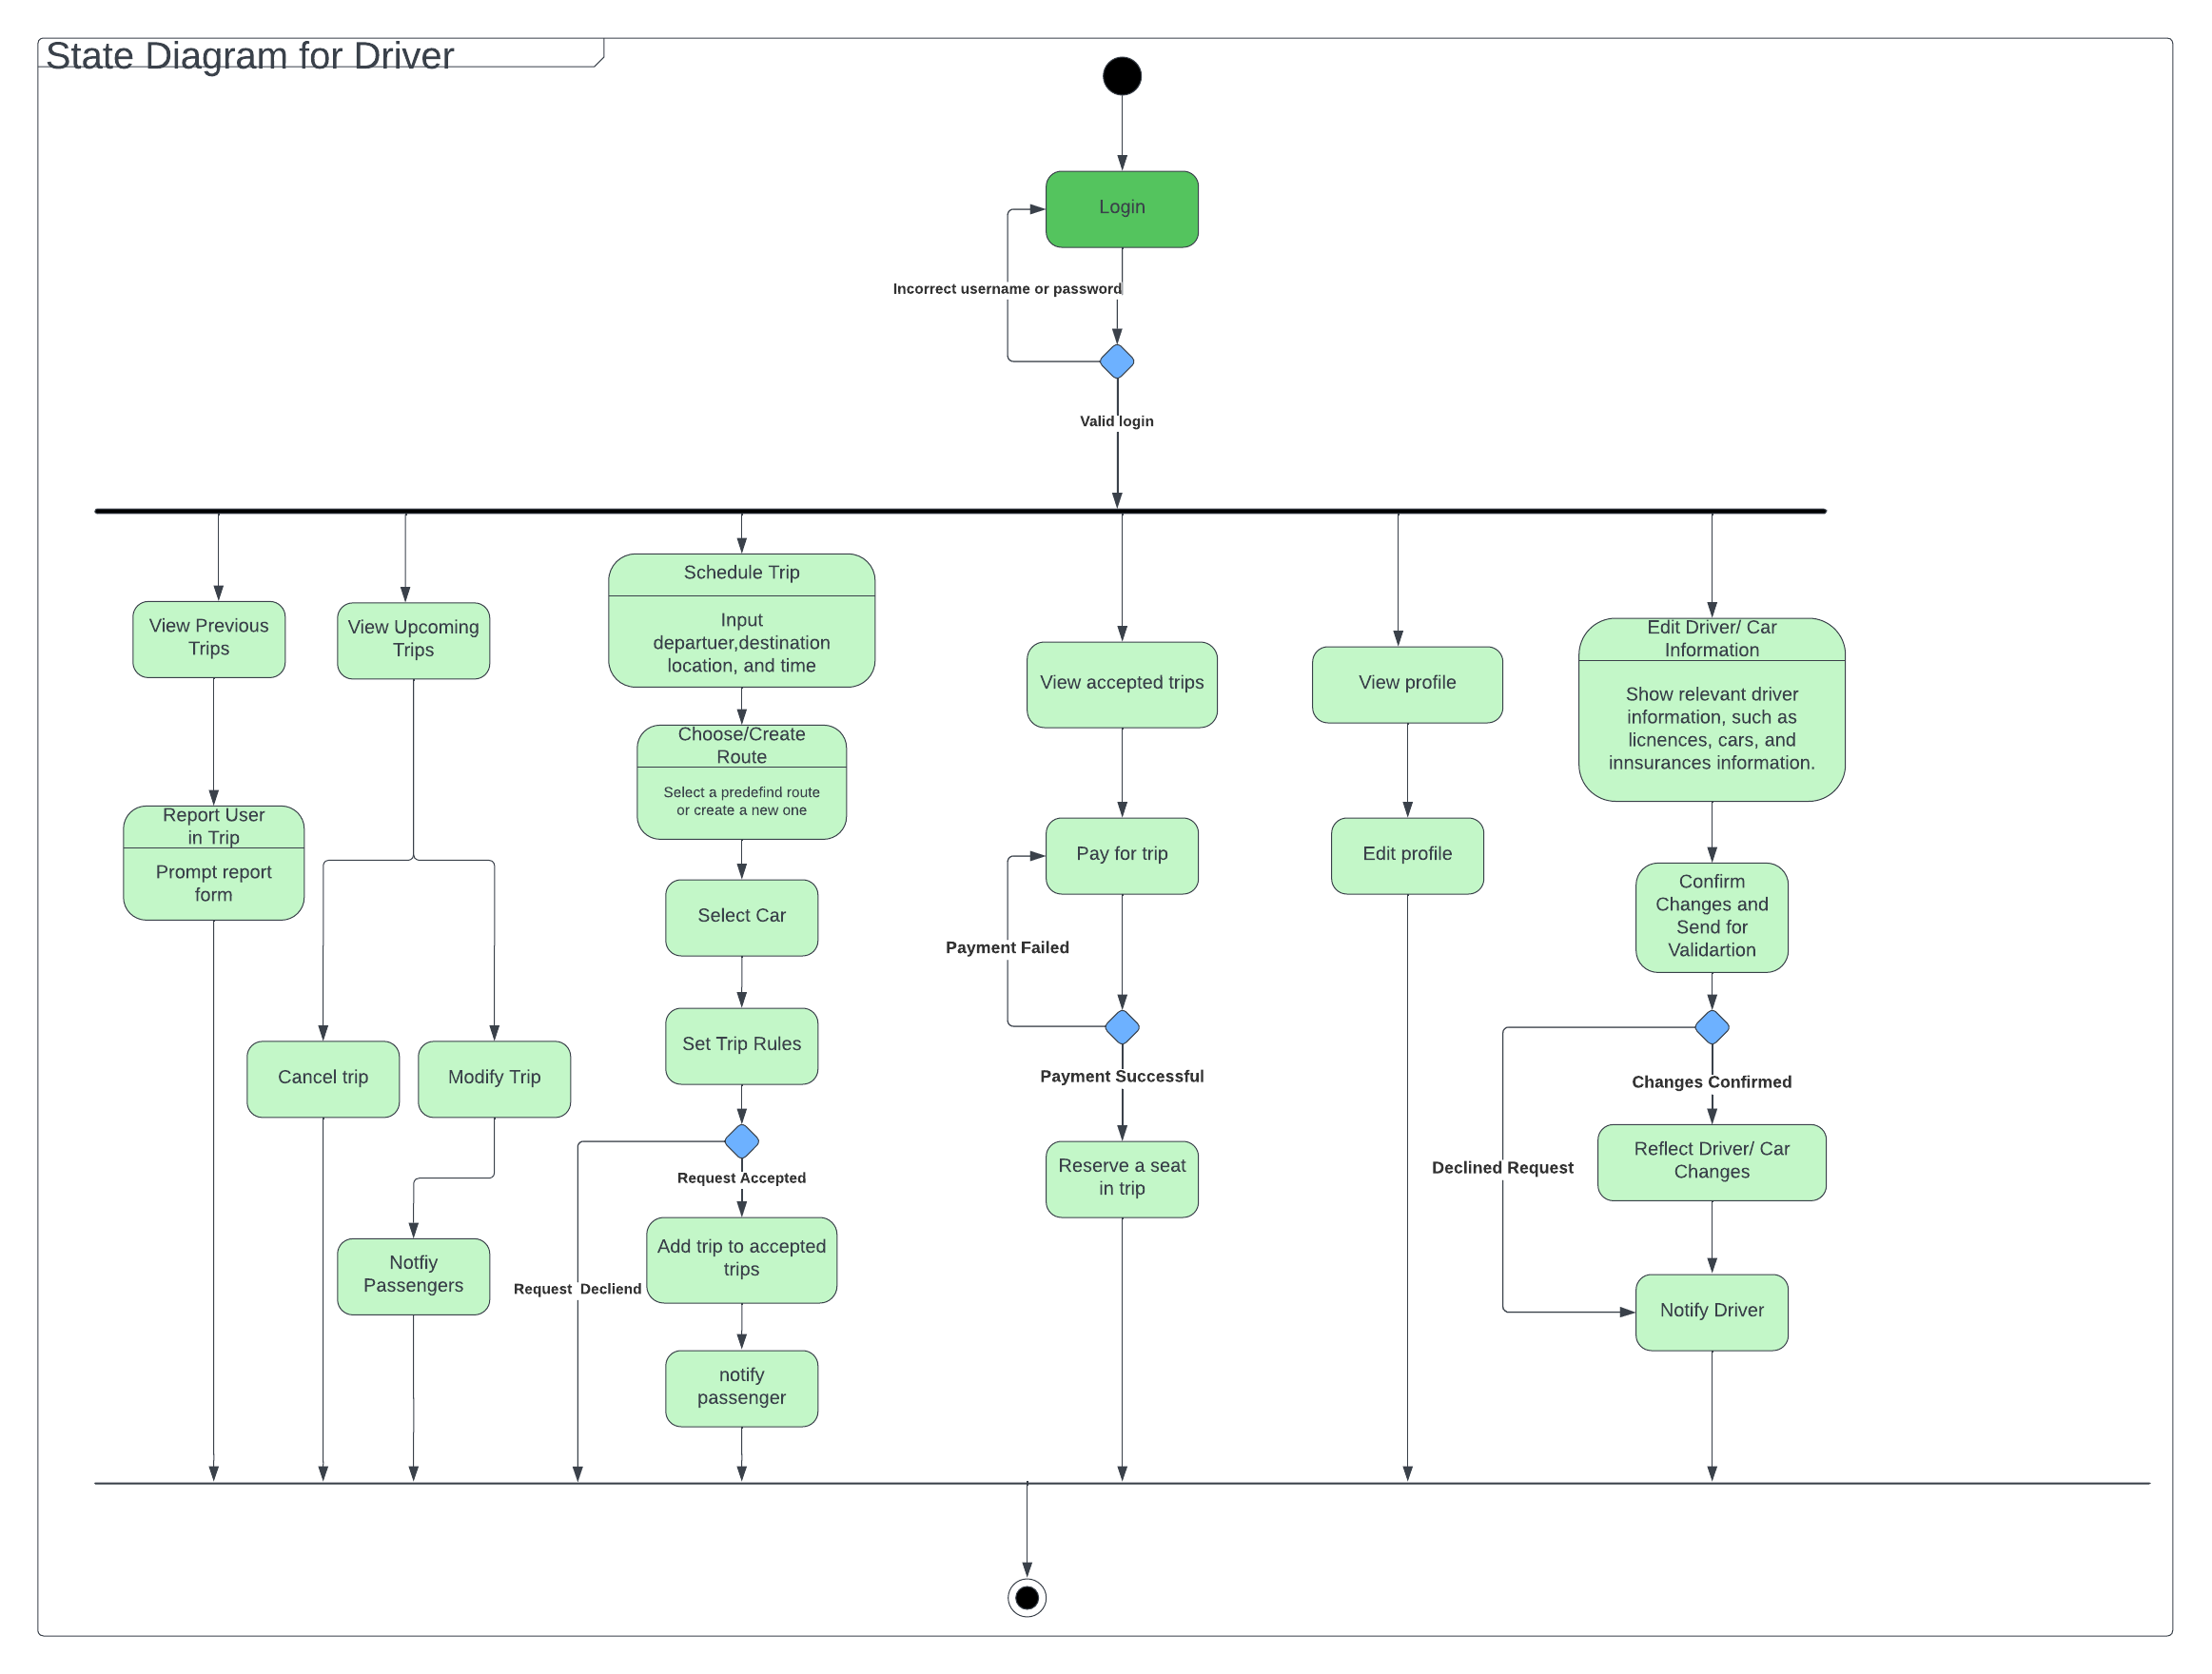
\includegraphics[width=\linewidth]{Images/State Diagram Driver.png}
            \caption{State Diagram for Driver}
            \label{fig:state_driver}
        \end{sidewaysfigure}

        \FloatBarrier

        \begin{sidewaysfigure}[!htb]
            \centering
            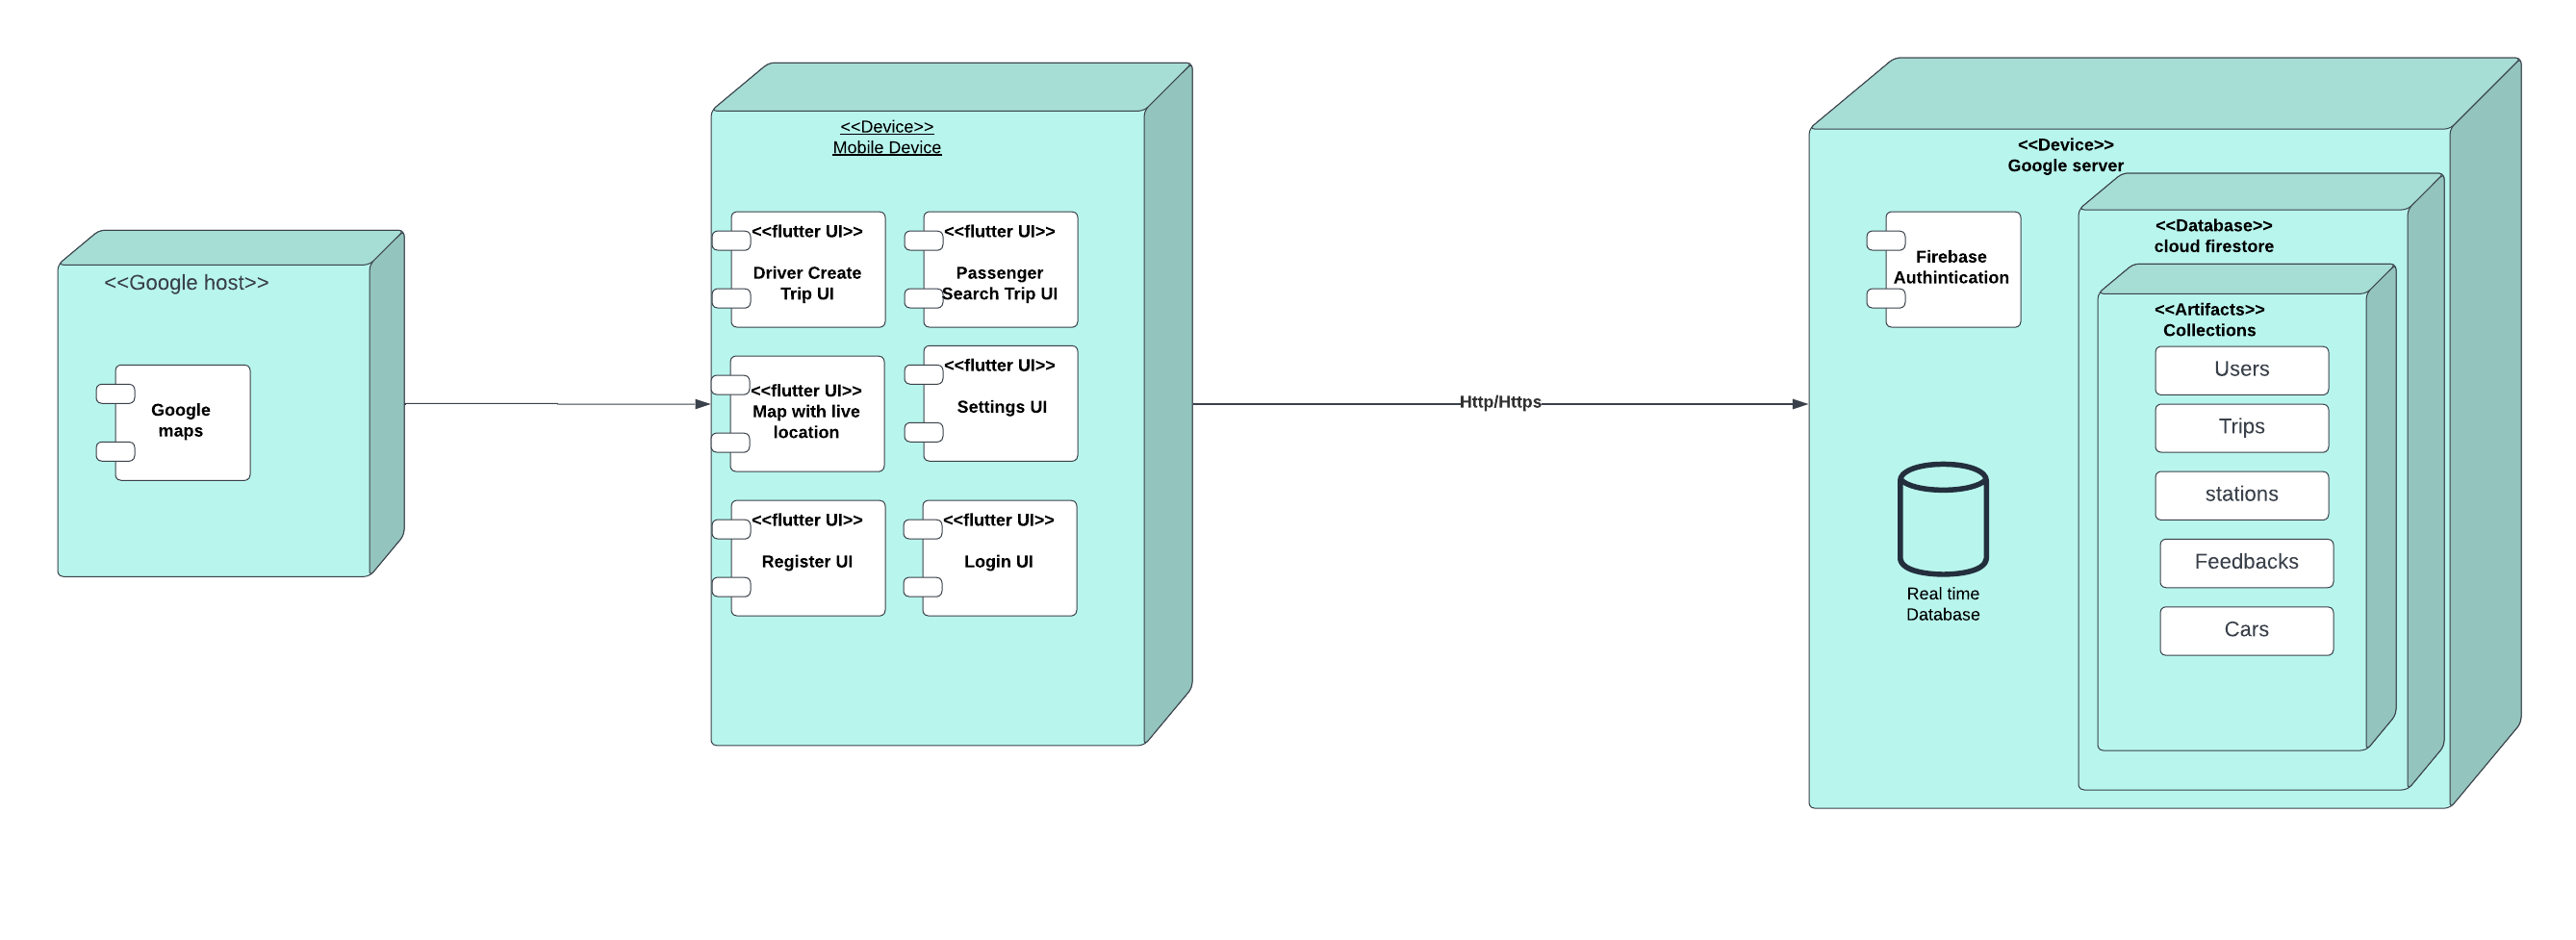
\includegraphics[width=\linewidth]{Images/deployment_diagram.png}
            \caption{Deployment Diagram}
            \label{fig:dep_diagram}
        \end{sidewaysfigure}

        \FloatBarrier
        

    % \section{Changes to Part 1 Requirements}
    % As we started working on the application, we found that Firebase has a lot of features that cover the functionalities of a designated backend. Therefore, for the time being, there is no need to create a Spring Boot API for our application. Firebase has a built in authentication system with password reset and email and phone verification. The database has filtering queries backend that enables us to send specialized requests to get, update, or create specific data. There are no other changes are currently for the rest of the requirements in part 1.

    \pagebreak
    \section{Implementation}
        \subsection{Introduction}
            This is a continuation of the first part of the project, which was dedicated to the analysis and design of the project, while this part is dedicated to the implementation and testing of the project. The project is a ridesharing app that allows people signed up as drivers to pick up passengers along the way with them to a mutual destination. The mobile application is built with flutter, and firebase as the backend and database servers.

            Since the workflow of the project is incremental, we started by working on the core features that our app depends on first. The core features of our app such as, backend building, searching for trips, booking trips logic, and account creation and authentication. Then we worked on providing map and location services to make it easier for drivers to create trips (pick stations) and for both drivers and passengers to easily find each other. In addition to that, we worked on user profiles, trip filters, and trip reviews. 
            
            Throughout these stages, we have worked on the UI and UX for each feature simultaneously. The final stage was to test the app. This section outlines some of the work we have done across stages 1 - 8 of implementation backlog found in Figure \ref{fig:work_plan}. It includes screenshot from the app running on both Android and iOS presenting the user interface and the features implemented.

            The application architecture consists of presentation, models, controllers, services, repositories, and others like assets and utility classes. Presentations are flutter stateless and stateful widgets which can be whole screens or building blocks used in the various screens of the application. Models represent the entity classes in the application like: stations, users, trips and others. Services and repositories following the Layered Architecture. Controllers are there to handle data being sent to the screens from one or more services. Most screens in our application have a controller. The assets consist of the in-memory images used in the application like the logo and default images. Utils and utility classes consists of different utility classes and functionalities that are shared across the application, for example logic to calculate distances between different points, shared providers like current user provider. We are using Riverpod state management to manage the state of the application (update widgets that rely on changed states).

        \pagebreak
        \subsection{Firebase Setup}
            We have set up the Firebase project and integrated it with the app. We have set up the Firebase Authentication, Storage, and FireStore Database. Figure \ref{fig:firebase_setup} shows the Firebase console with the Authentication methods enabled for for our and some of the documents stored in the FireStore Database.
            \begin{figure}[H]
                \centering
                \begin{subfigure}{0.7\textwidth}
                    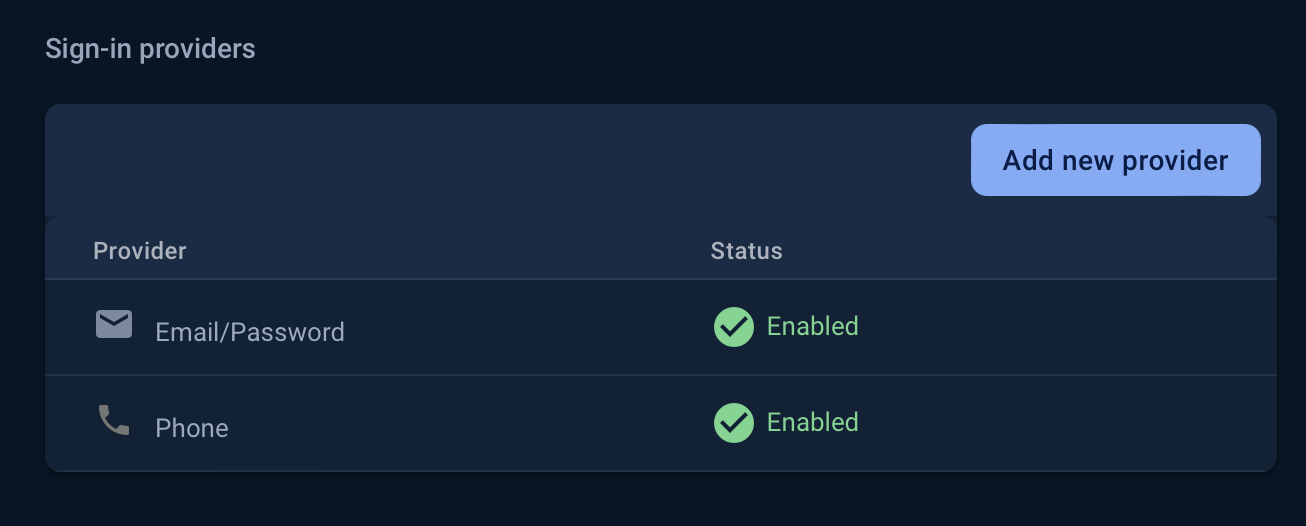
\includegraphics[width=\linewidth]{Images/firebase_auth.png}
                    \caption{Firebase Authentication}
                    \label{fig:firebase_auth}
                \end{subfigure}
                \begin{subfigure}{0.7\textwidth}
                    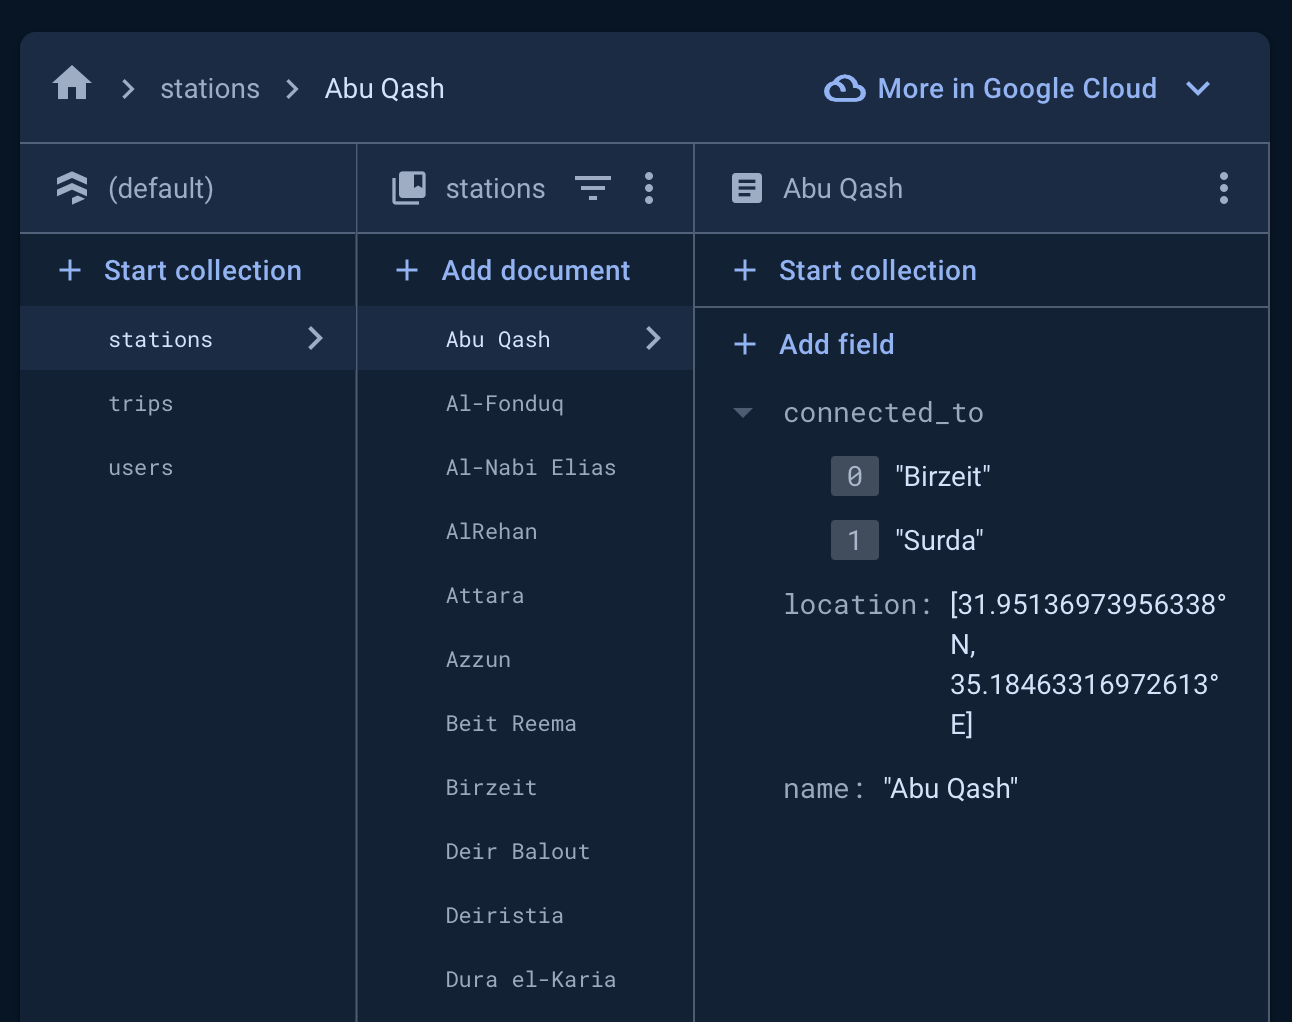
\includegraphics[width=\linewidth]{Images/firestore.png}
                    \caption{Firebase FireStore Database}
                    \label{fig:firebase_database}
                \end{subfigure}
                \caption{Firebase Console}
                \label{fig:firebase_setup}
            \end{figure}
        
        \pagebreak
        \subsection{User Sign up and Login}
            We have implemented the user sign up and login functionalities using Firebase Authentication. The user can currently sign up using their email. They will need to verify their email to be able to login. Email verification as well as password reset are implemented. Figure \ref{fig:real_sign_up_login} shows the start screen the user sign up screen and login screens. Guest accounts, and phone sign up are not implemented yet.
            \begin{figure}[H]
                \centering
                \begin{subfigure}{0.3\textwidth}
                    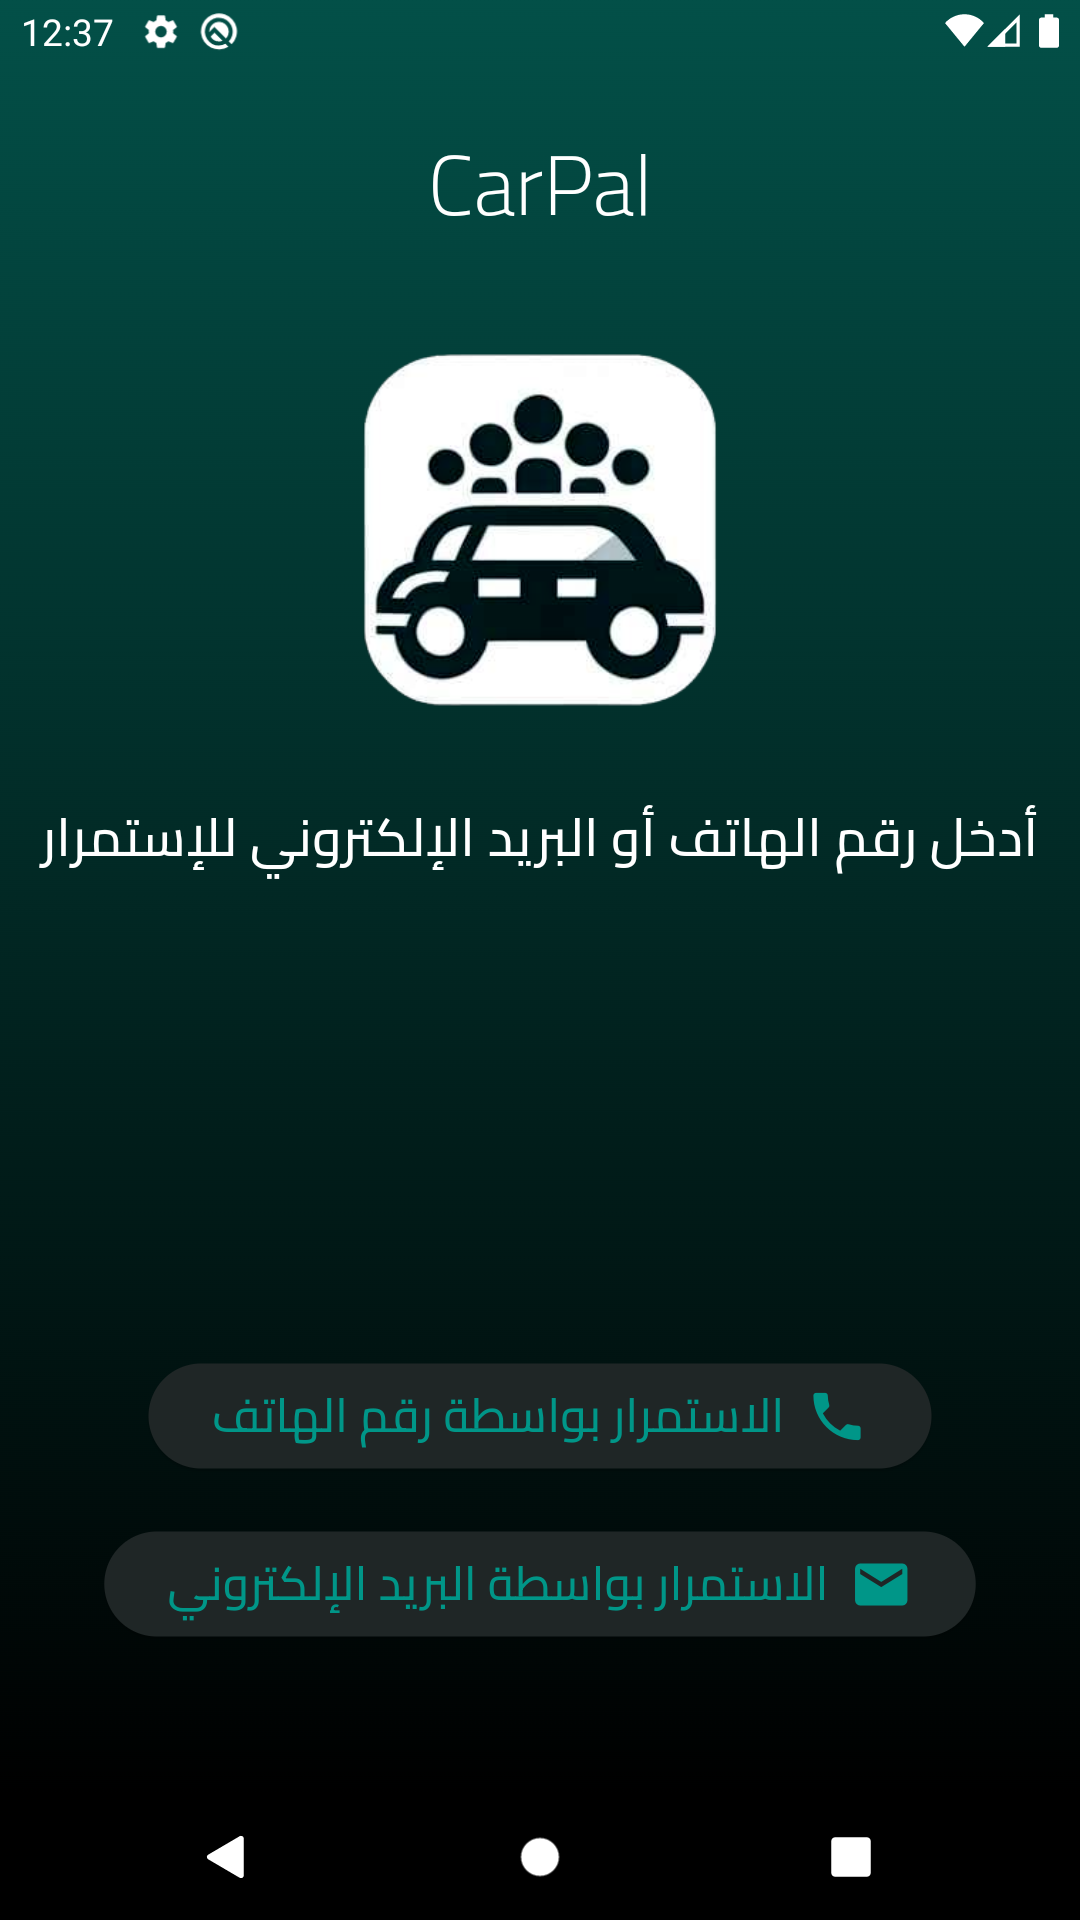
\includegraphics[width=0.8\linewidth, height=0.9\textheight, keepaspectratio]{Images/first_screen.png}
                    \caption{App Start Screen}
                    \label{fig:real_first_screen}
                \end{subfigure}
                \begin{subfigure}{0.3\textwidth}
                    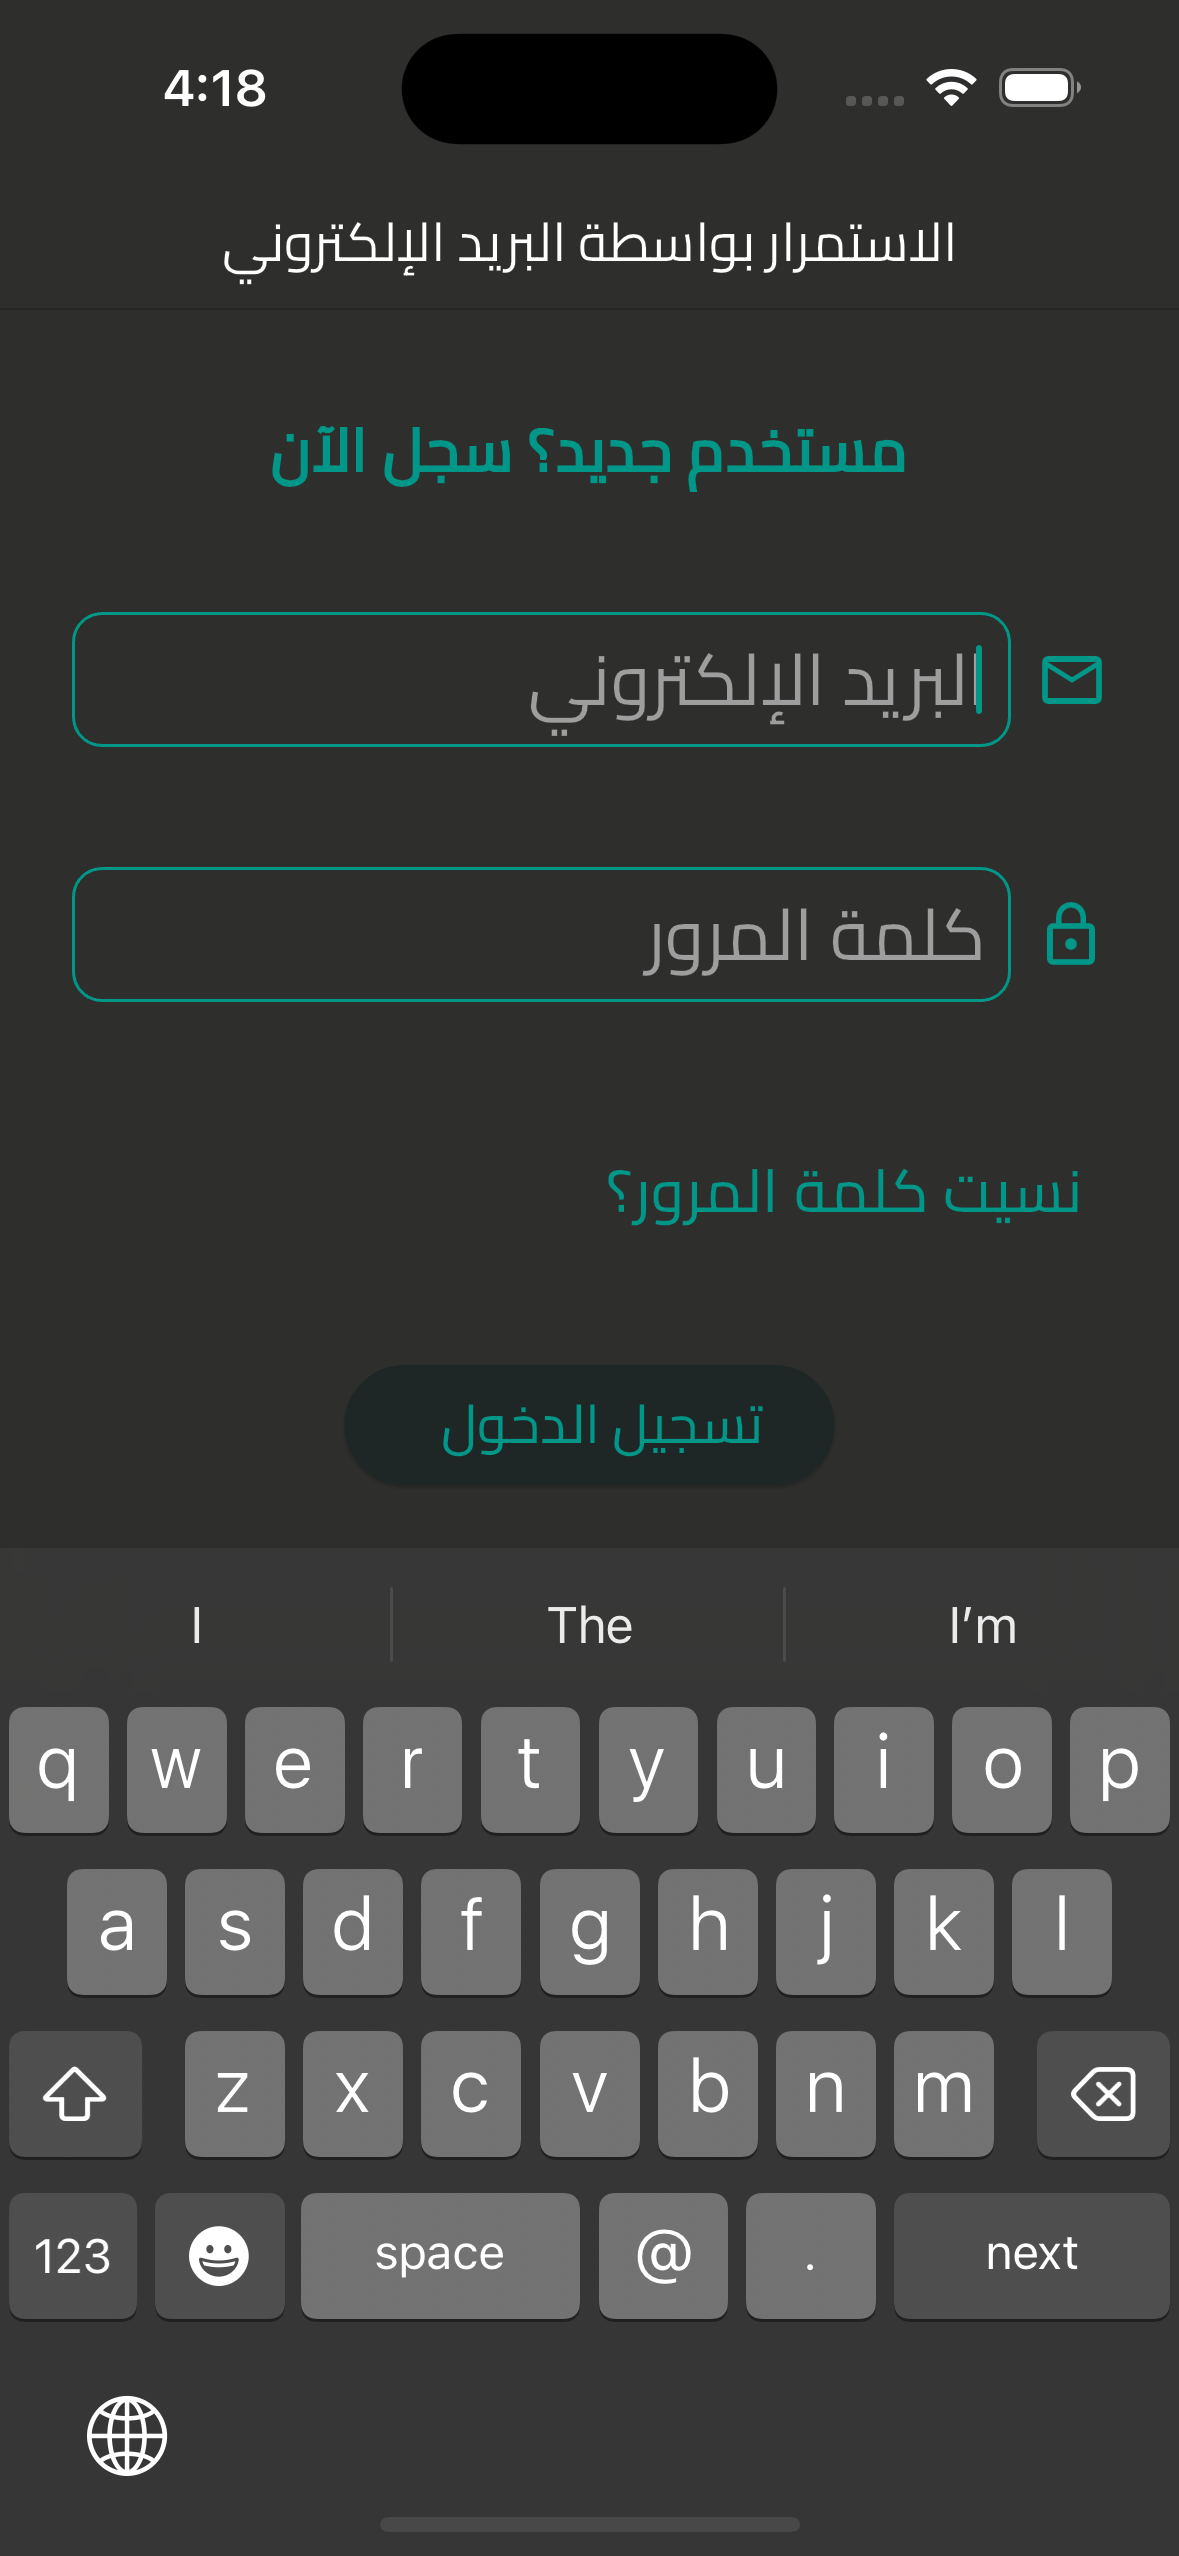
\includegraphics[width=0.8\linewidth, height=0.9\textheight, keepaspectratio]{Images/user_login.png}
                    \caption{Login Screen - iOS}
                    \label{fig:real_login}
                \end{subfigure}
                \begin{subfigure}{0.3\textwidth}
                    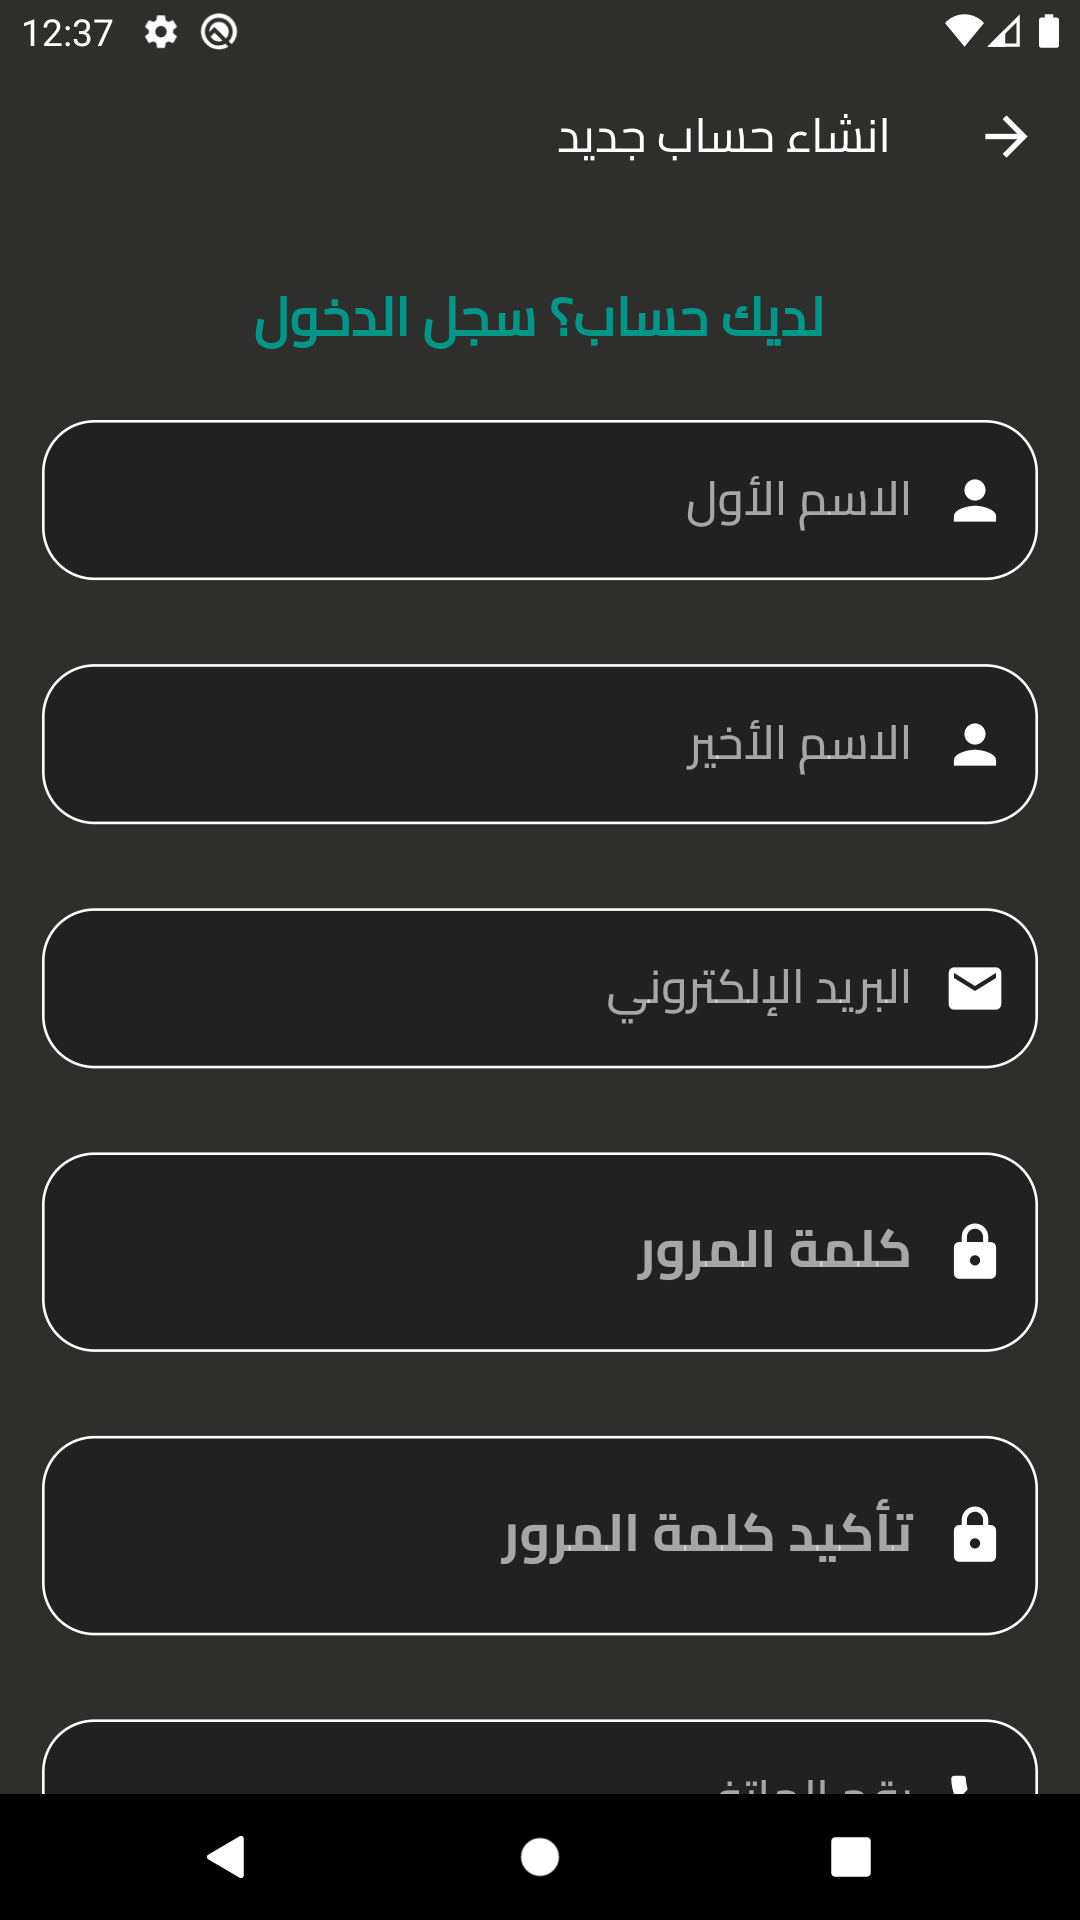
\includegraphics[width=0.8\linewidth, height=0.9\textheight, keepaspectratio]{Images/user_sign_up_1.png}
                    \caption{Sign Up Screen - Android}
                    \label{fig:real_sign_up_1}
                \end{subfigure}
                \begin{subfigure}{0.3\textwidth}
                    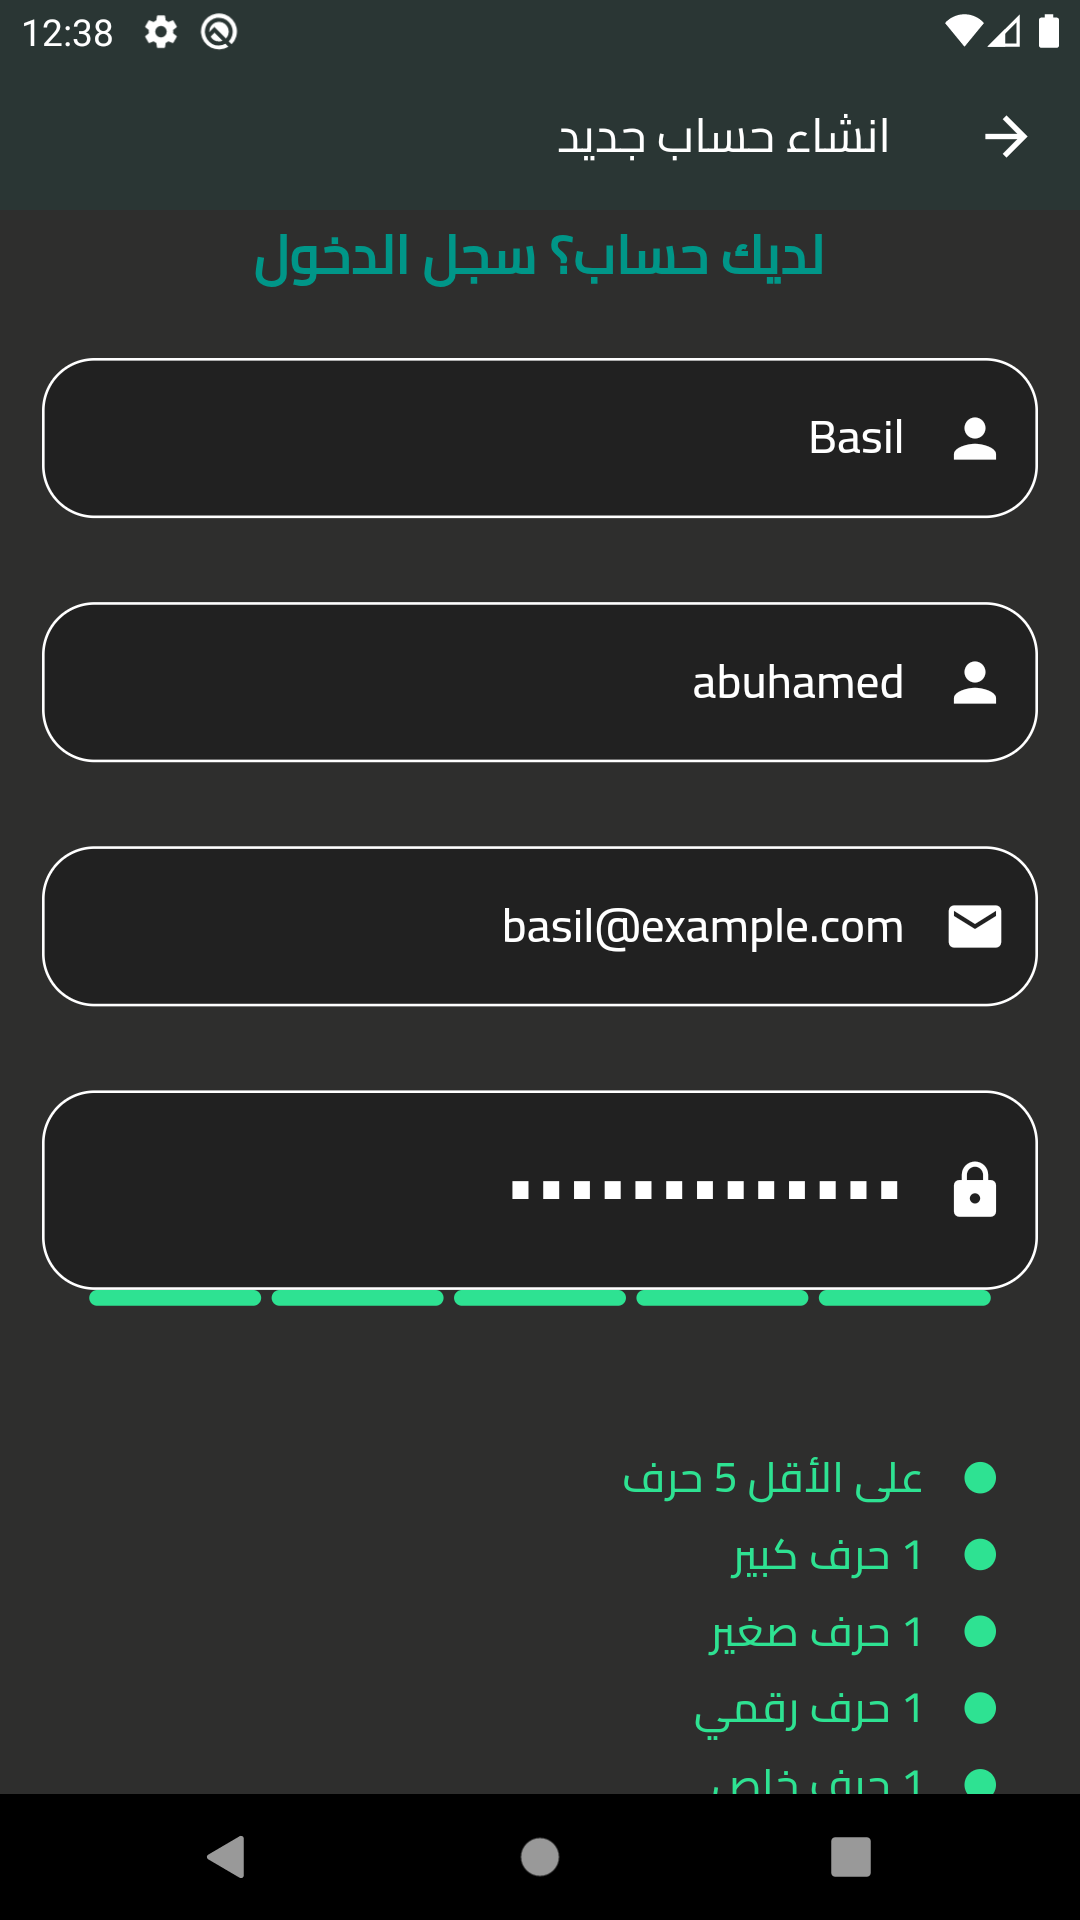
\includegraphics[width=0.8\linewidth, height=0.9\textheight, keepaspectratio]{Images/user_sign_up_2.png}  
                    \caption{Sign Up Screen with Password Validation - Android}
                    \label{fig:real_sign_up_2}
                \end{subfigure}
                \begin{subfigure}{0.3\textwidth}
                    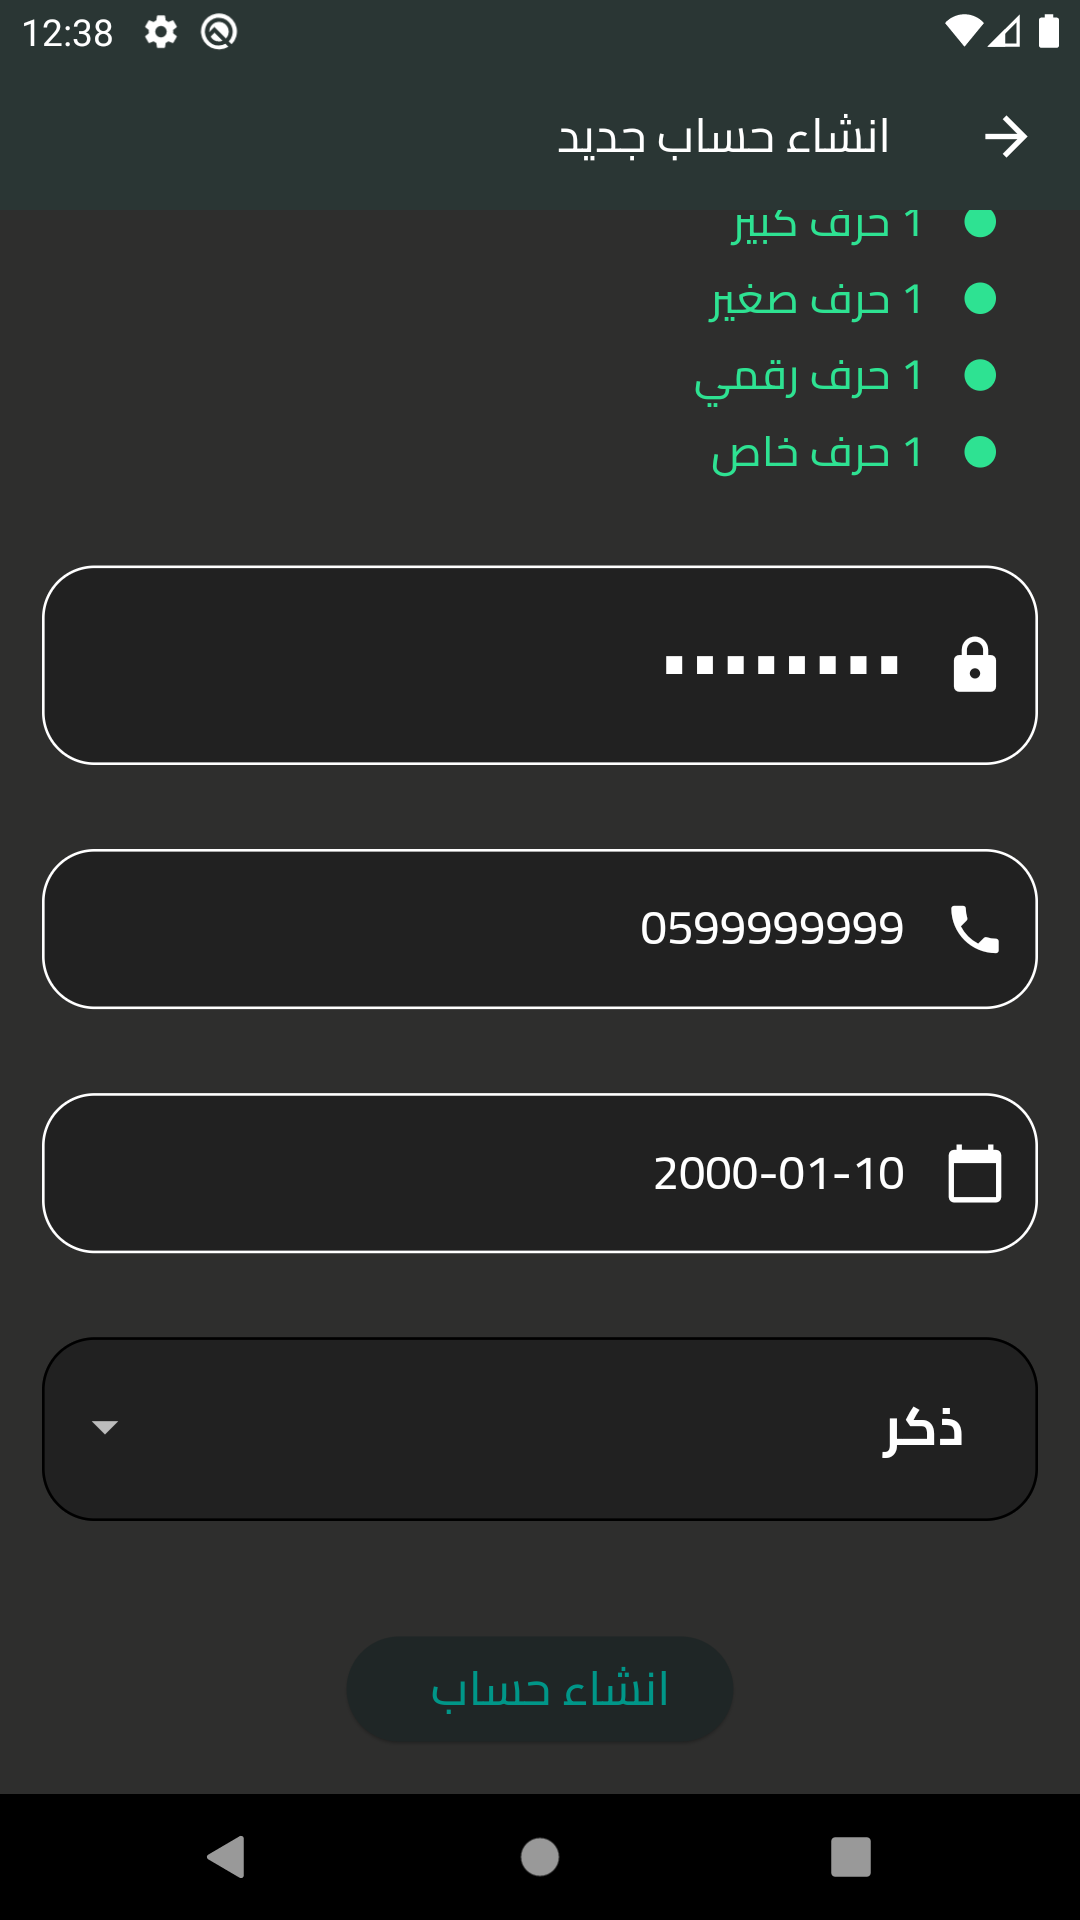
\includegraphics[width=0.8\linewidth, height=0.9\textheight, keepaspectratio]{Images/user_sign_up_3.png}
                    \caption{Cont. Sign Up Screen - Android}
                    \label{fig:real_sign_up_3}
                \end{subfigure}
                \begin{subfigure}{0.3\textwidth}
                    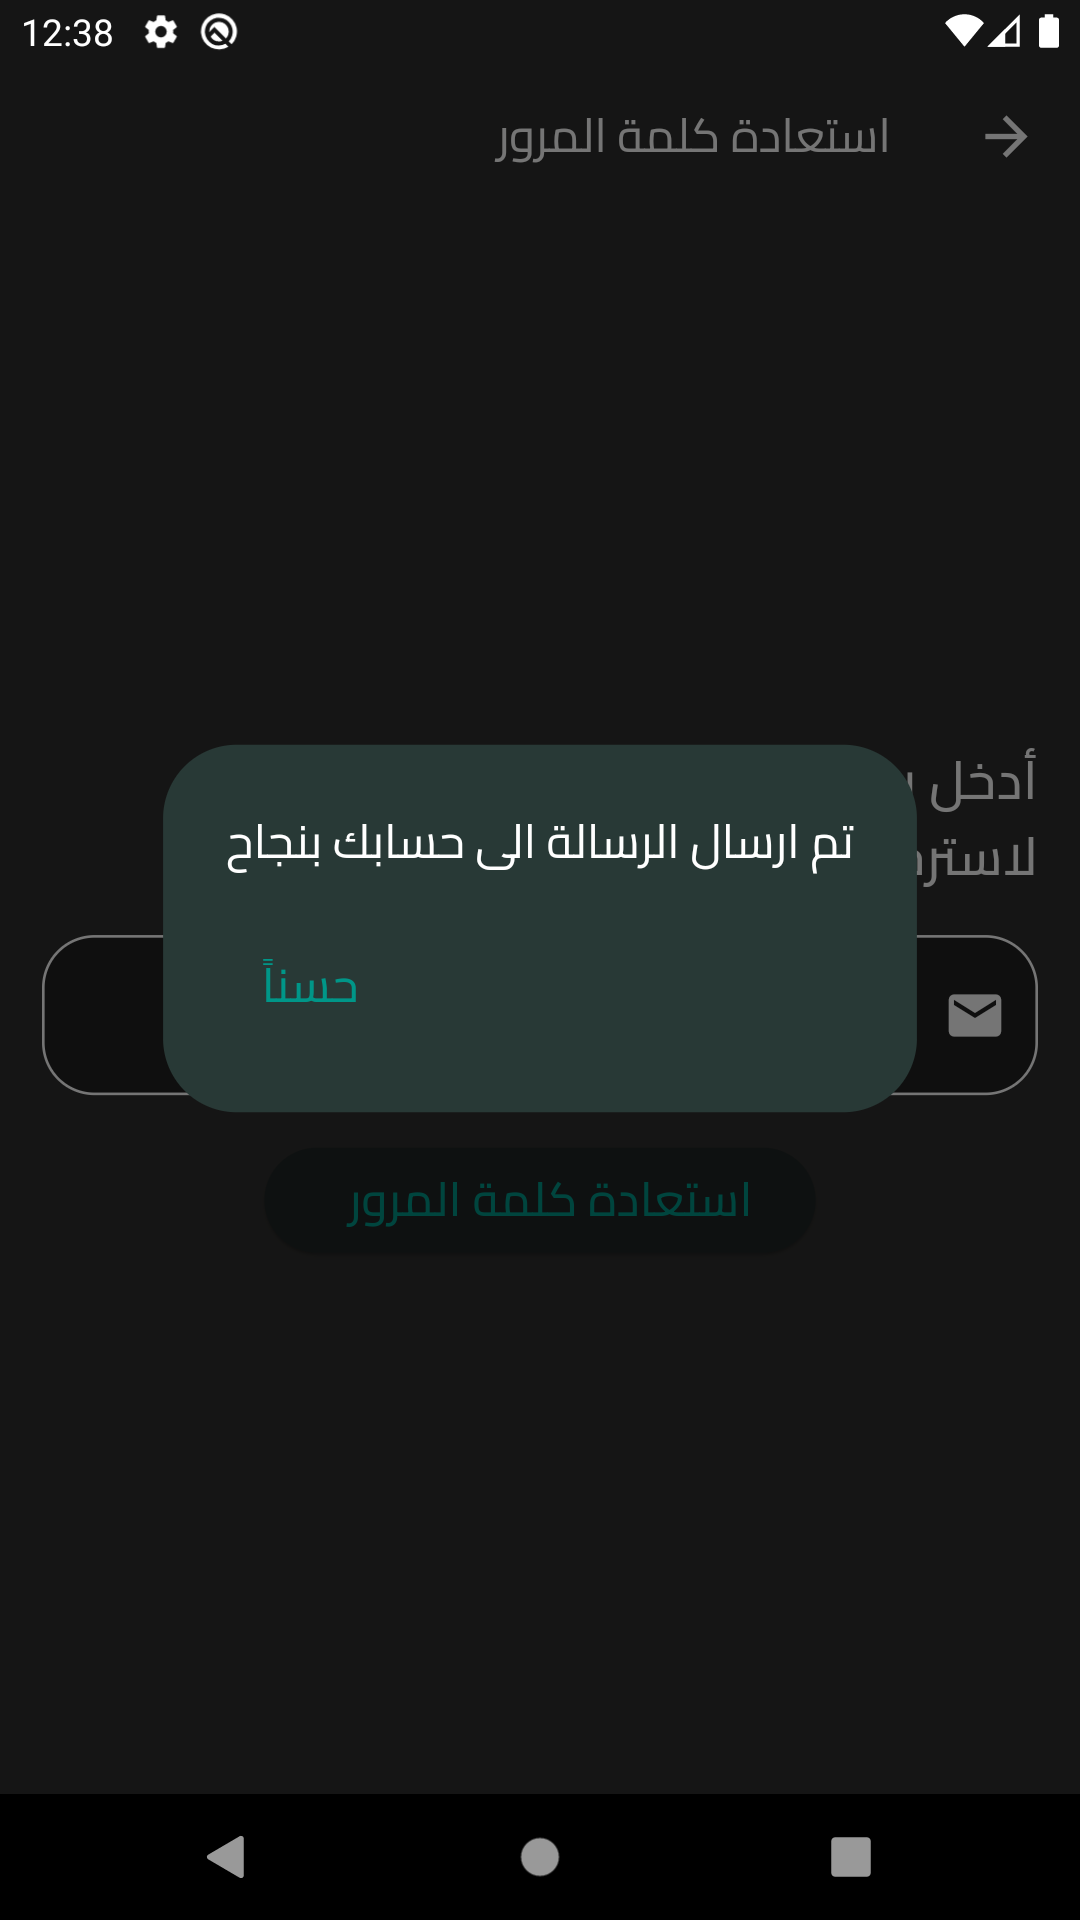
\includegraphics[width=0.8\linewidth, height=0.9\textheight, keepaspectratio]{Images/password_reset.png}
                    \caption{Password Reset - Android}
                    \label{fig:password_reset}
                \end{subfigure}
                \caption{User Sign Up and Login Screens}
                \label{fig:real_sign_up_login}
            \end{figure}

        \subsection{Driver Trip Creation}
            Drivers can create trips by specifying the departure and destination locations, time of the trip, available seats, and the price of the trip. Further options such as trip rules and the stations to pass by are not implemented yet. Figure \ref{fig:trip_creation} shows the trip creation screens.
            \begin{figure}[H]
                \centering
                \begin{subfigure}{0.3\textwidth}
                    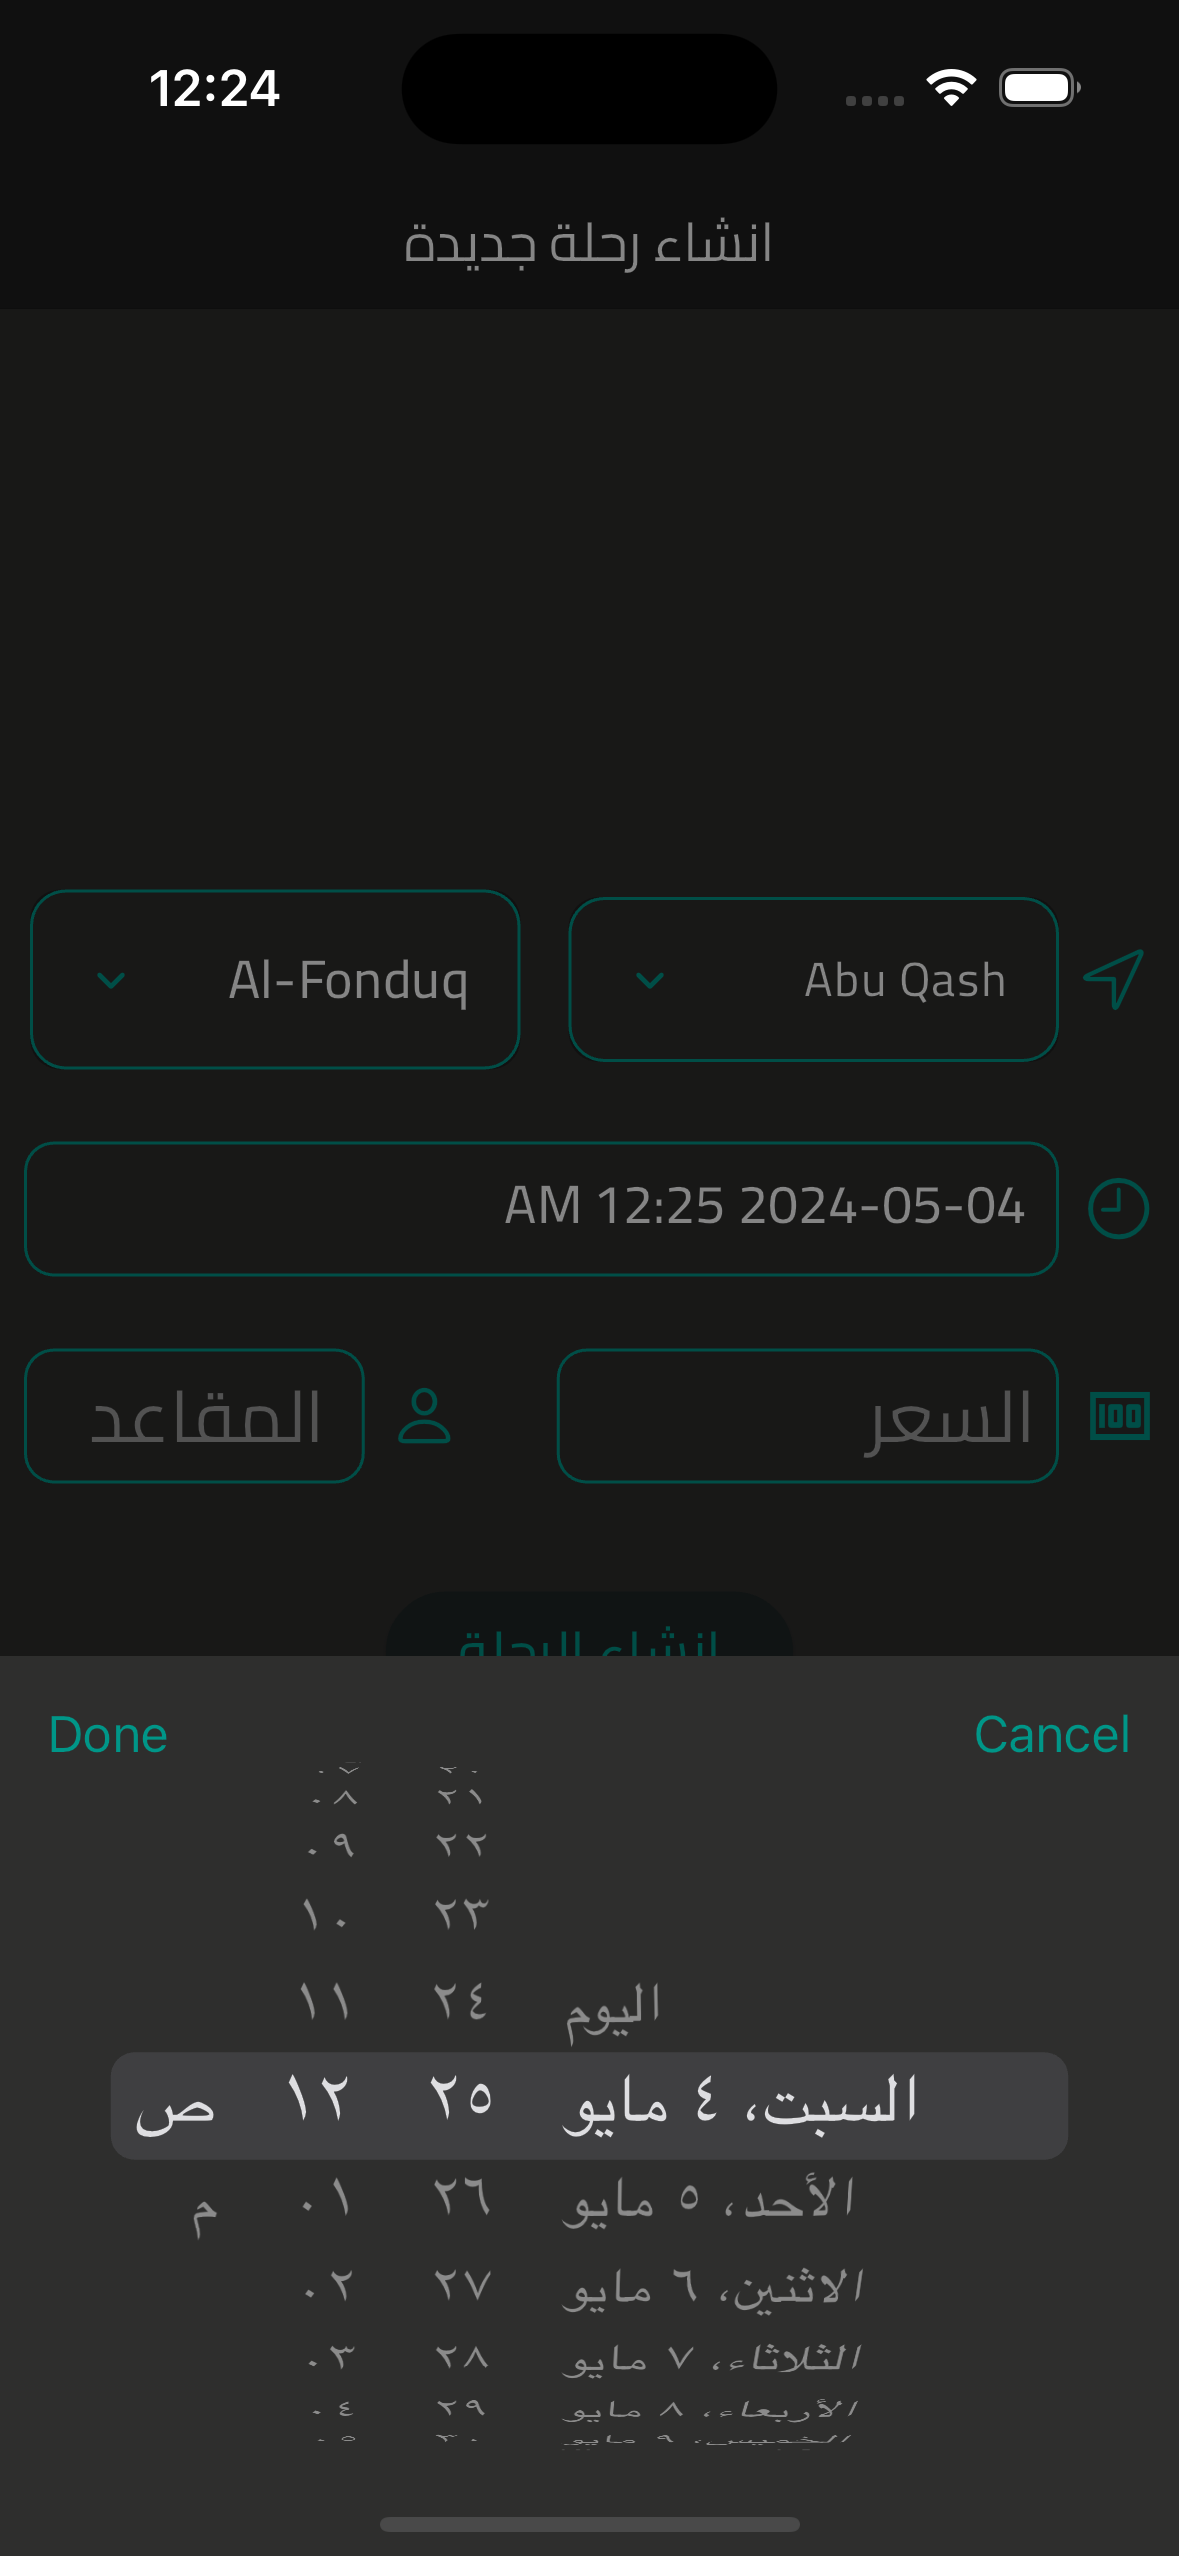
\includegraphics[width=\linewidth]{Images/trip_creation_1.png}
                    \caption{Trip Creation - iOS}
                    \label{fig:trip_cration_1}
                \end{subfigure}
                \begin{subfigure}{0.3\textwidth}
                    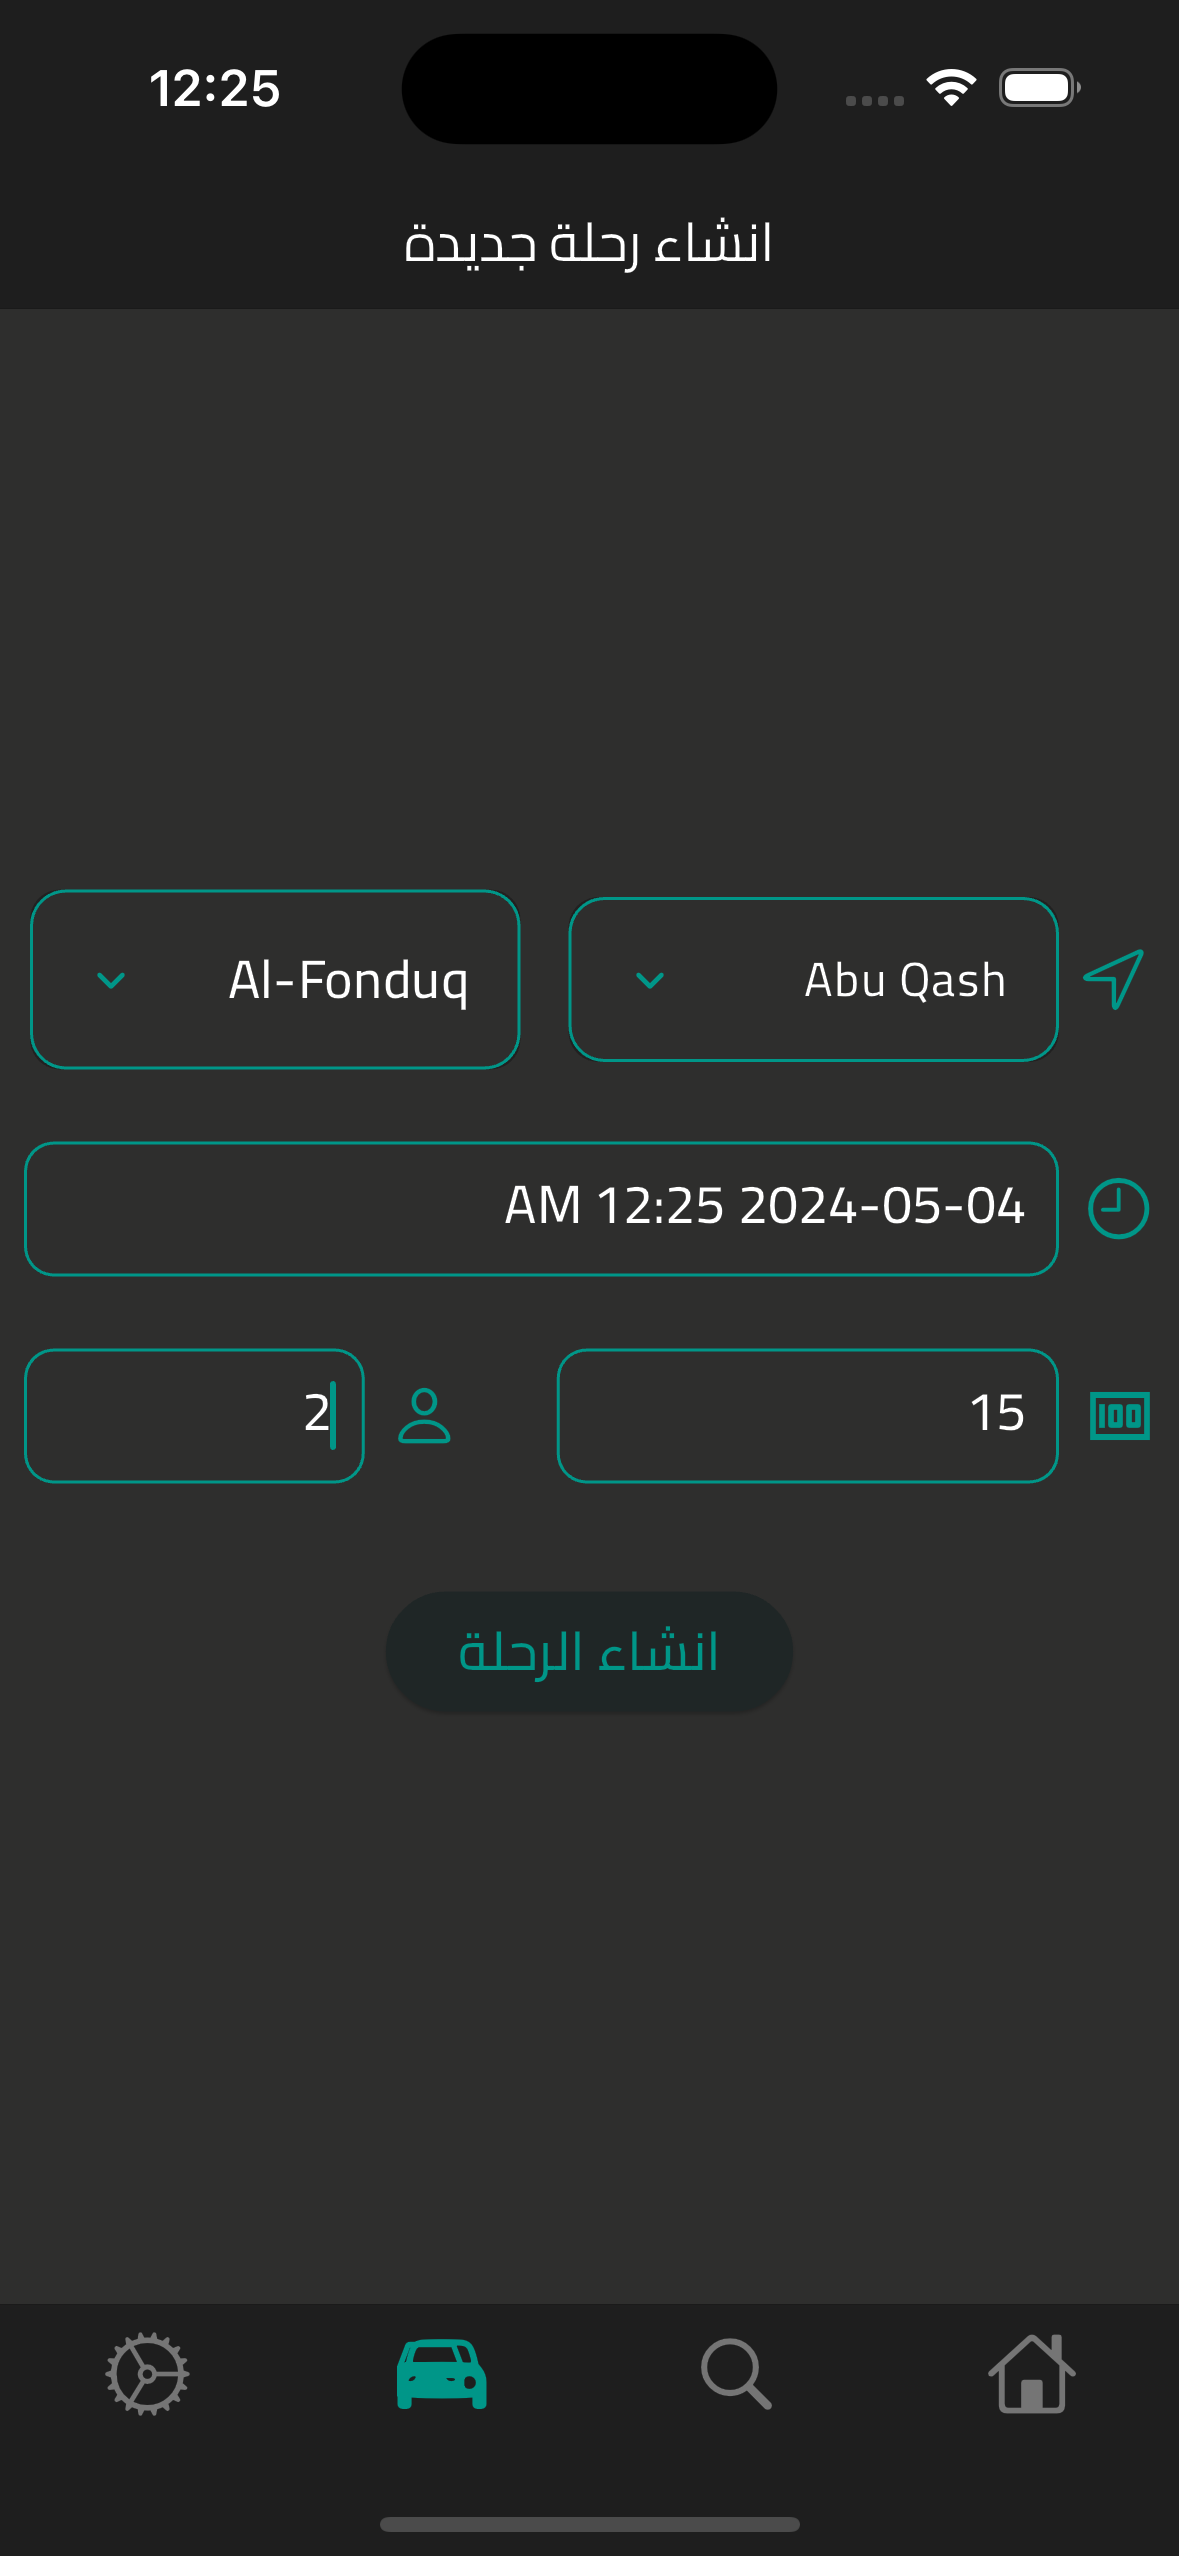
\includegraphics[width=\linewidth]{Images/trip_creation_2.png}
                    \caption{Cont. Trip Creation - iOS}
                    \label{fig:trip_cration_2}
                \end{subfigure}
                \begin{subfigure}{0.3\textwidth}
                    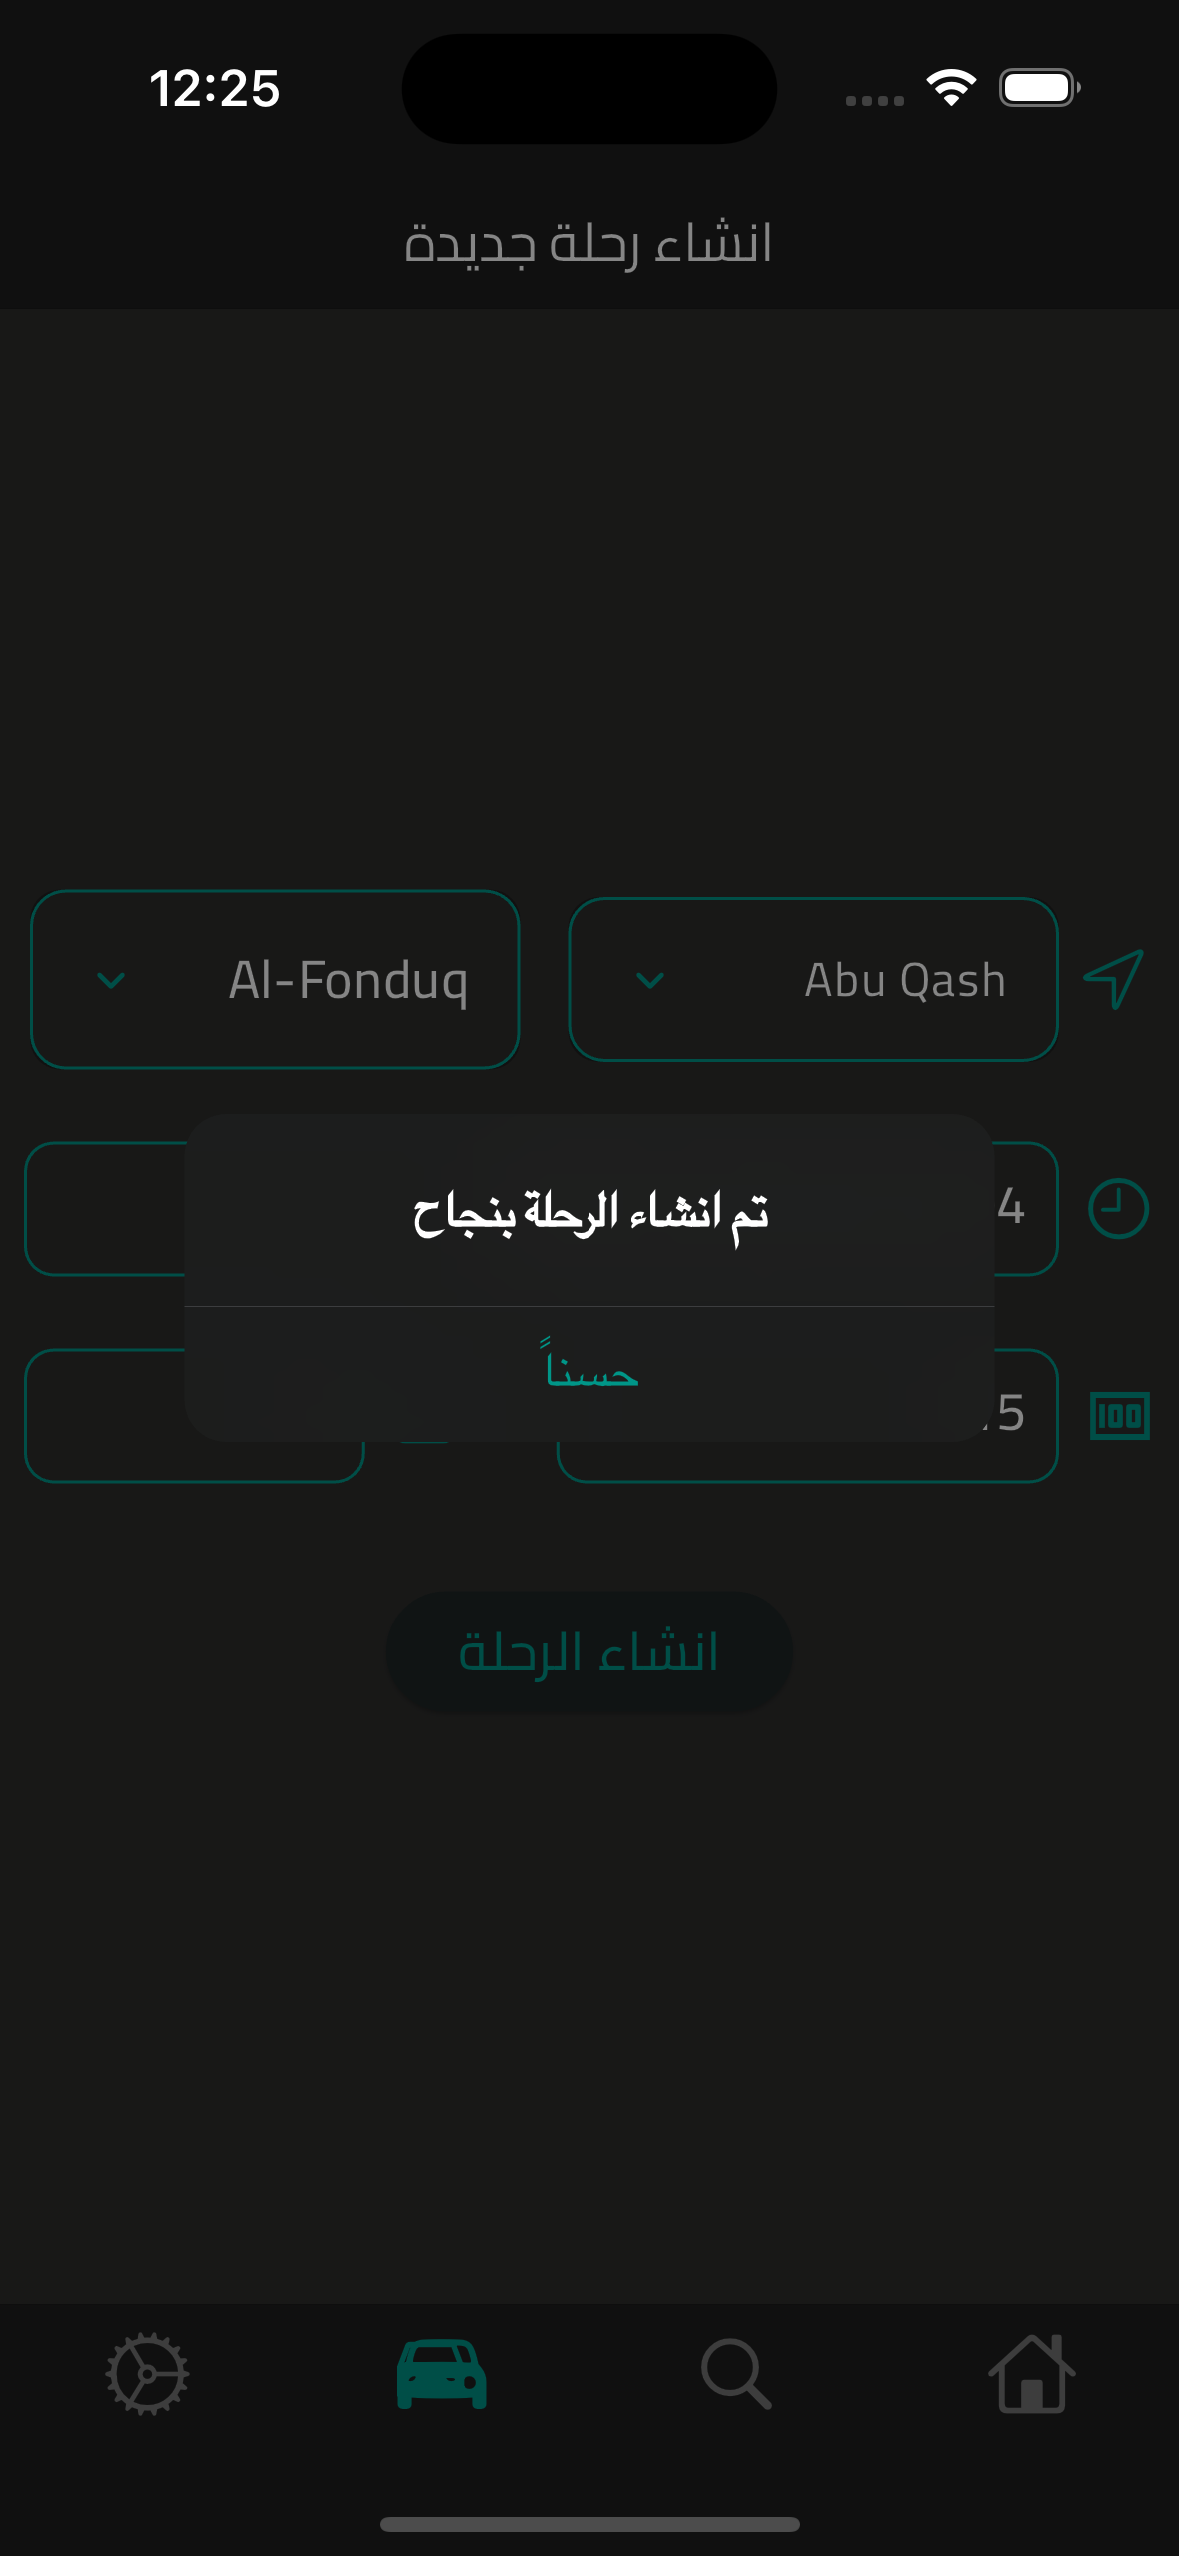
\includegraphics[width=\linewidth]{Images/trip_creation_3.png}  
                    \caption{Cont. Trip Creation - iOS}
                    \label{fig:trip_cration_3}
                \end{subfigure}
                \caption{Driver Trip Creation Screens}
                \label{fig:trip_creation}
            \end{figure}
        
        \pagebreak
        \subsection{Passenger Trip Search}
            The passengers can search for a trip using the \textit{Trip Search Screen}. Similar to the \textit{Trip Creation Screen} in UI and parameters, the passenger can search for the trip by entering the departure and destination locations, date of the trip, and the number of passengers that need to be accommodated When a search query is submitted, the app will open a new screen where the passenger can see the trips available and a map of the last location the driver was seen in. The passenger can pull down to refresh the page and update the trip list. In addition to the information visible in the trip list which can be seen in Figure \ref{fig:trip_search}, the trip list will also include information about the current driver location such the last time the location was updated. The trip list should also be sorted by different parameters (chosen by user) such time, price, distance, filters, and ratings. Each item in the trip list is clickable. The click action will open a new screen with more details about the trip, driver, and booked passengers if any. The \textit{Trip Detail Screen} will also include a map of the driver's last known location, extra information about the trip, such as passing stations, and the driver's rules if exists, and the driver's picture and rating, estimated time of arrival at each station, and total expected time of the trip. The passenger can book a trip by clicking the book button on the trip detail screen.
            \begin{figure}[H]
                \centering
                \begin{subfigure}{0.31\textwidth}
                    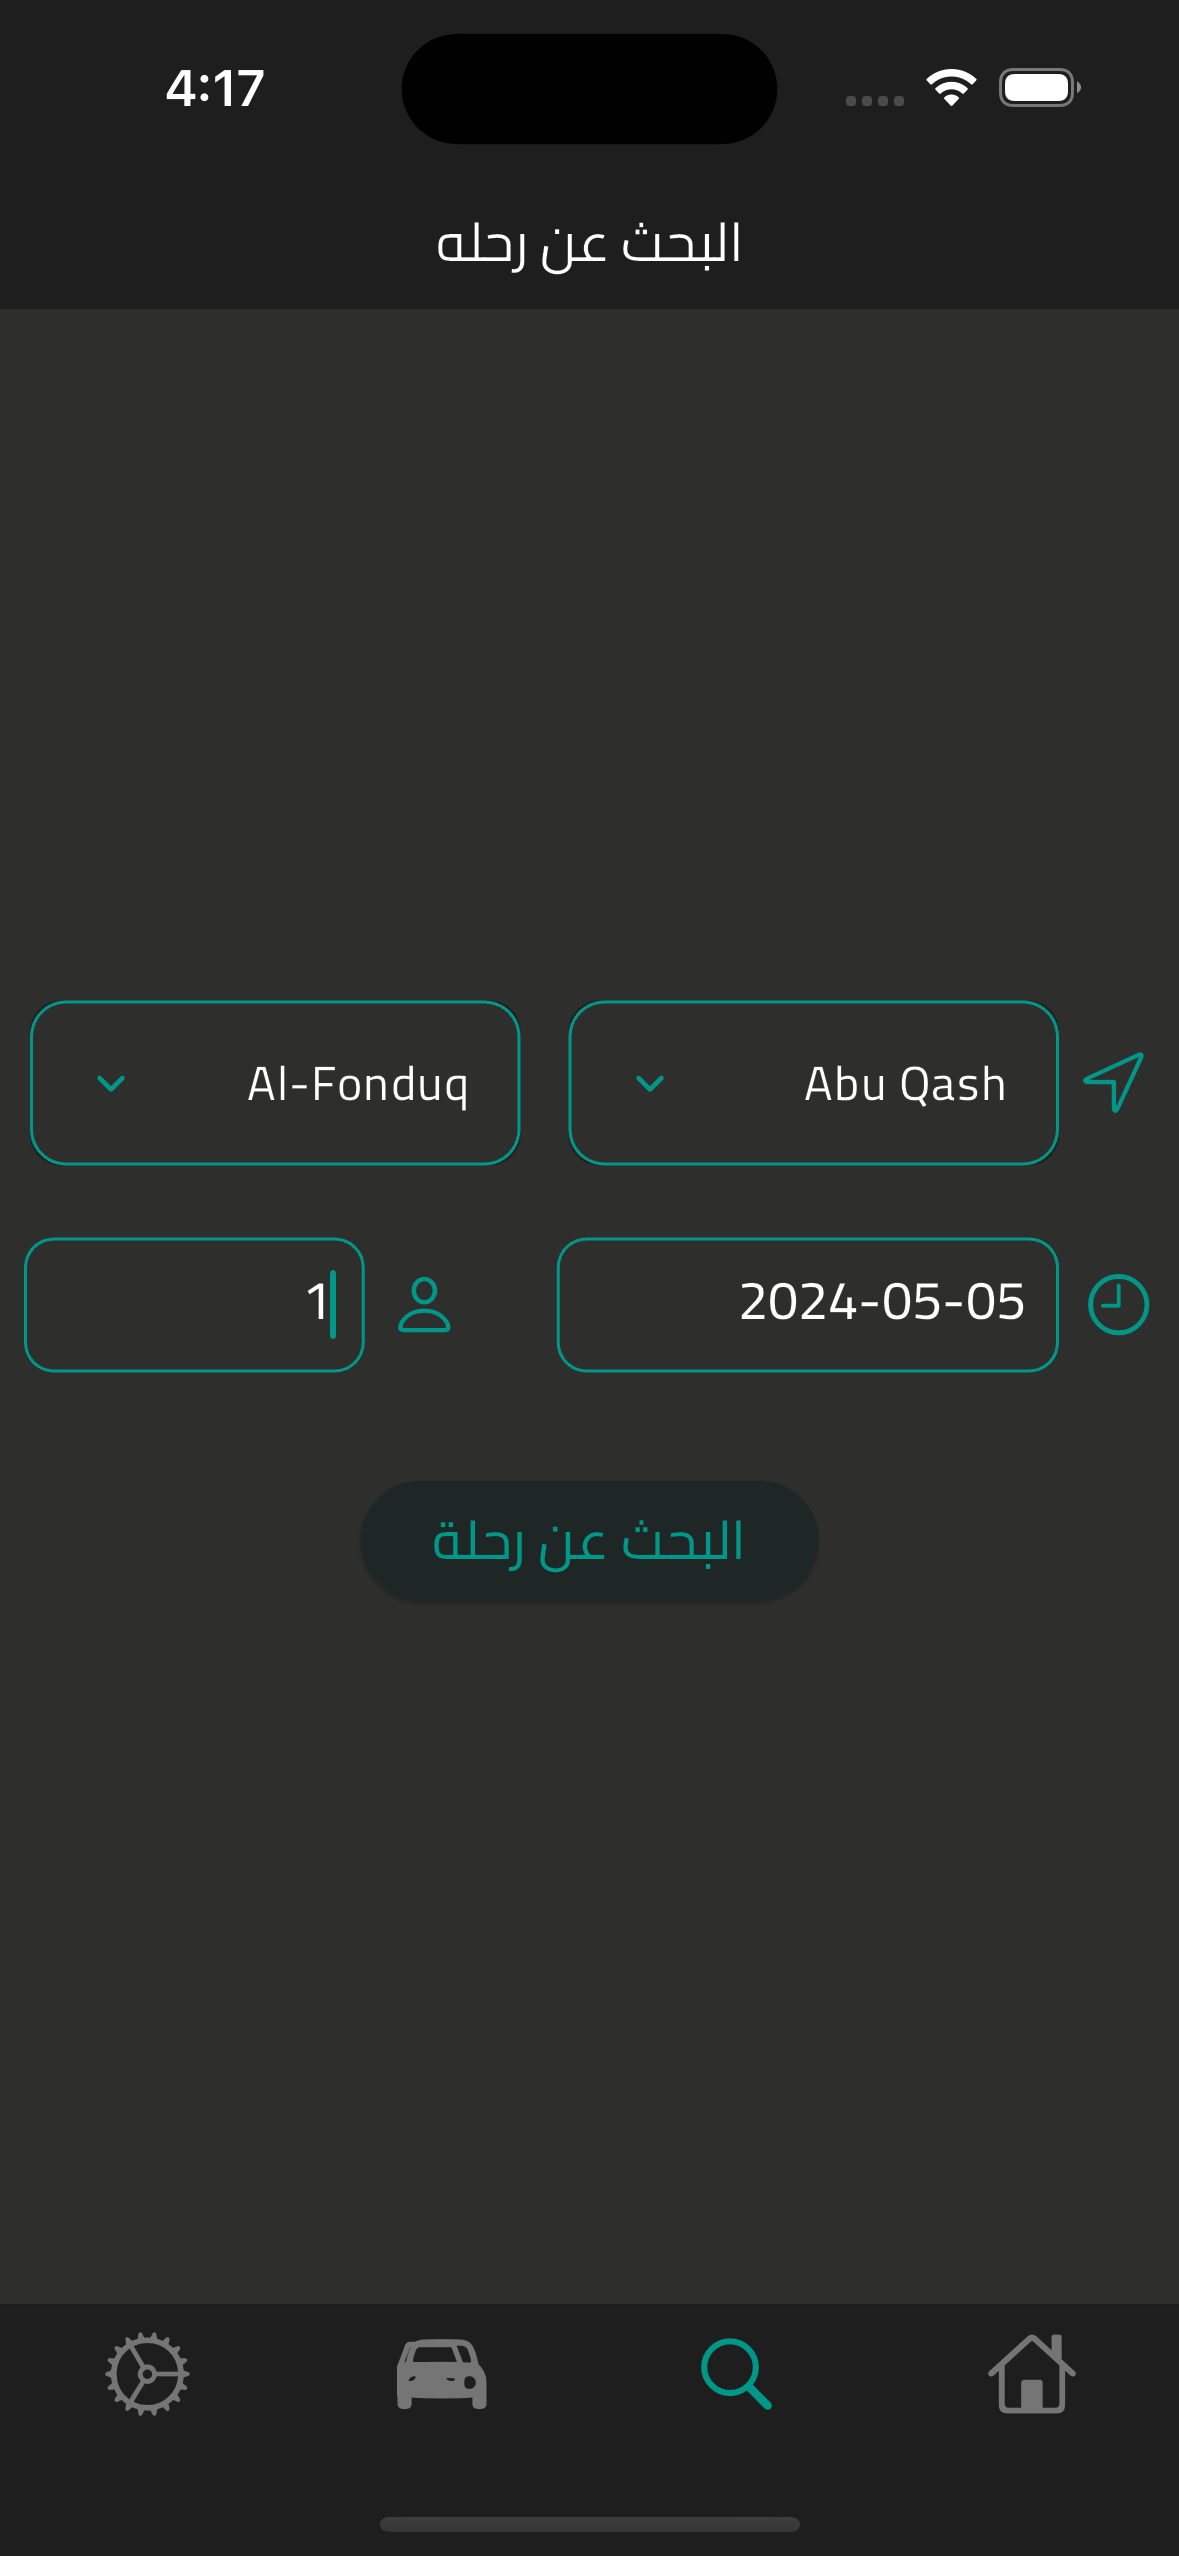
\includegraphics[width=\linewidth]{Images/trip_search_1.png}
                    \caption{Trip Search - iOS}
                    \label{fig:trip_search_1}
                \end{subfigure}
                \begin{subfigure}{0.31\textwidth}
                    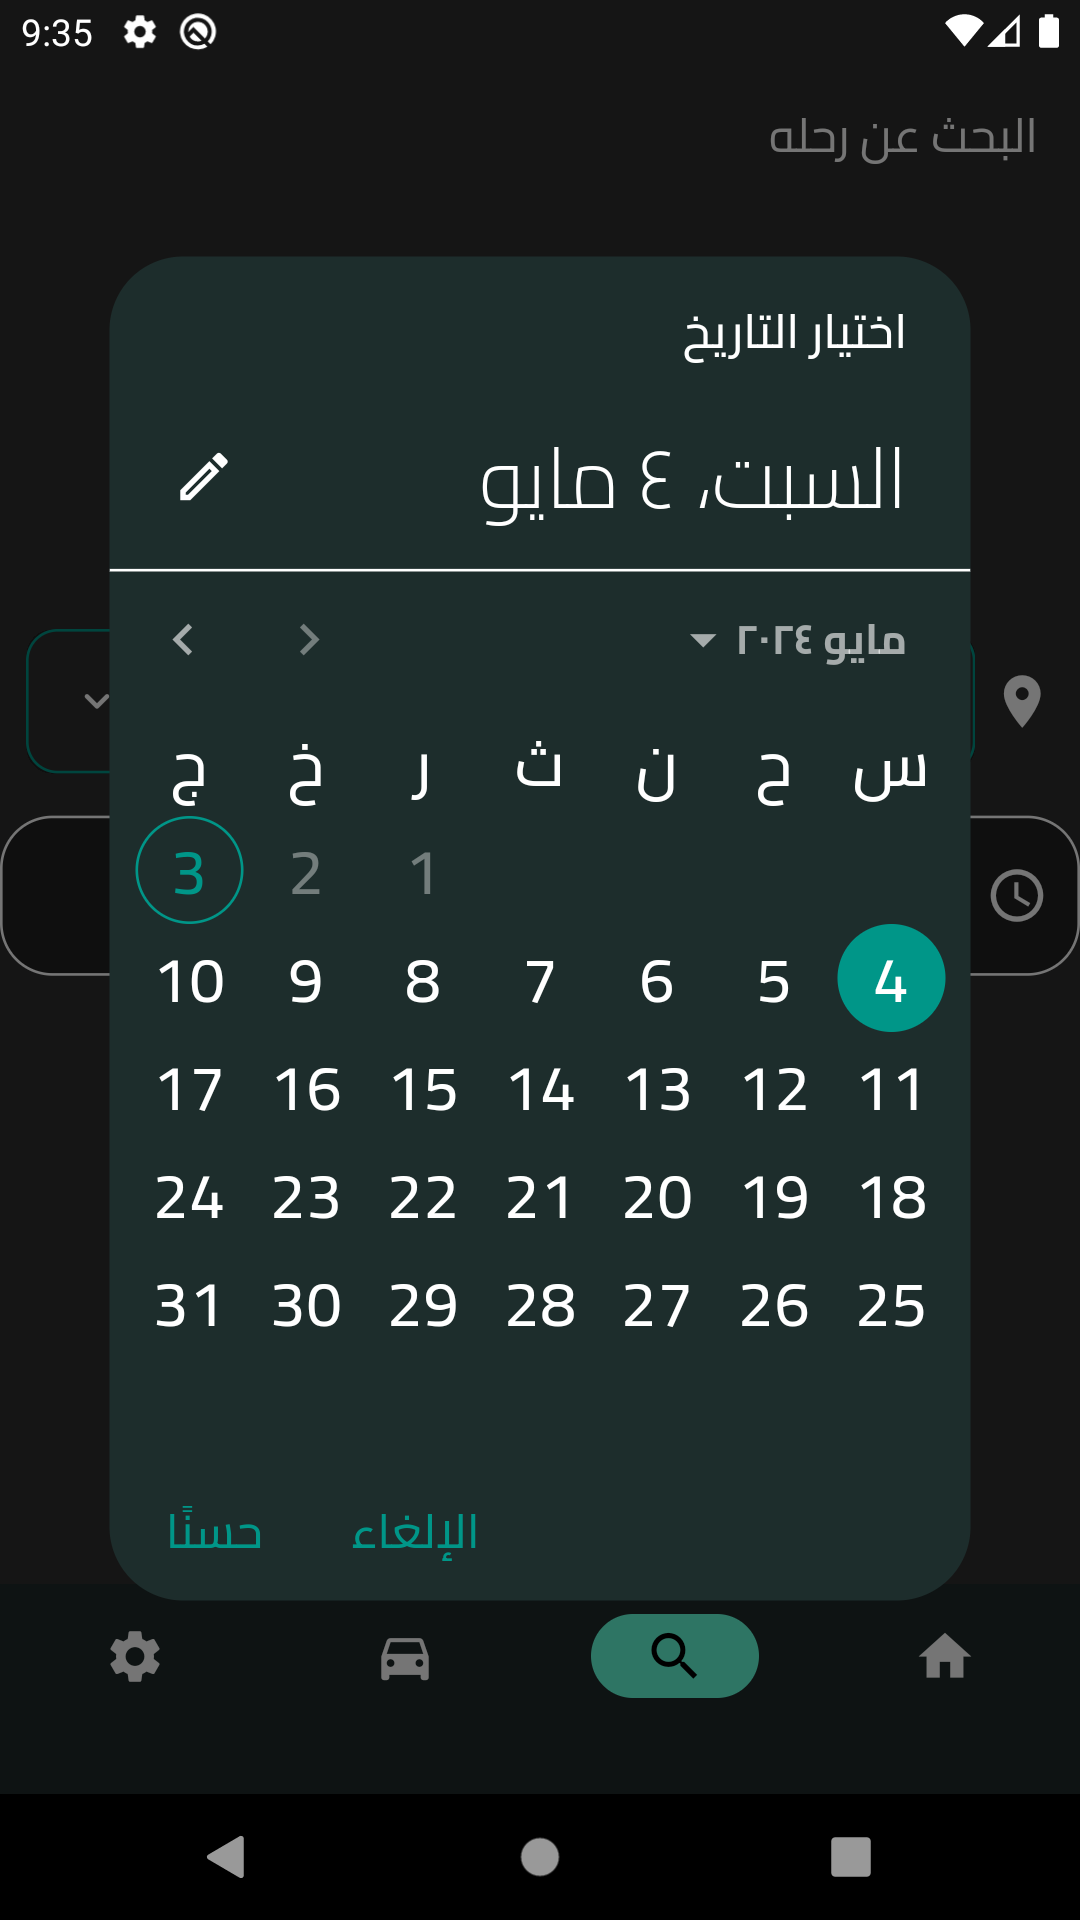
\includegraphics[width=\linewidth]{Images/trip_search_2.png}
                    \caption{Trip Search - Android}
                    \label{fig:trip_search_2}
                \end{subfigure}
                \begin{subfigure}{0.31\textwidth}
                    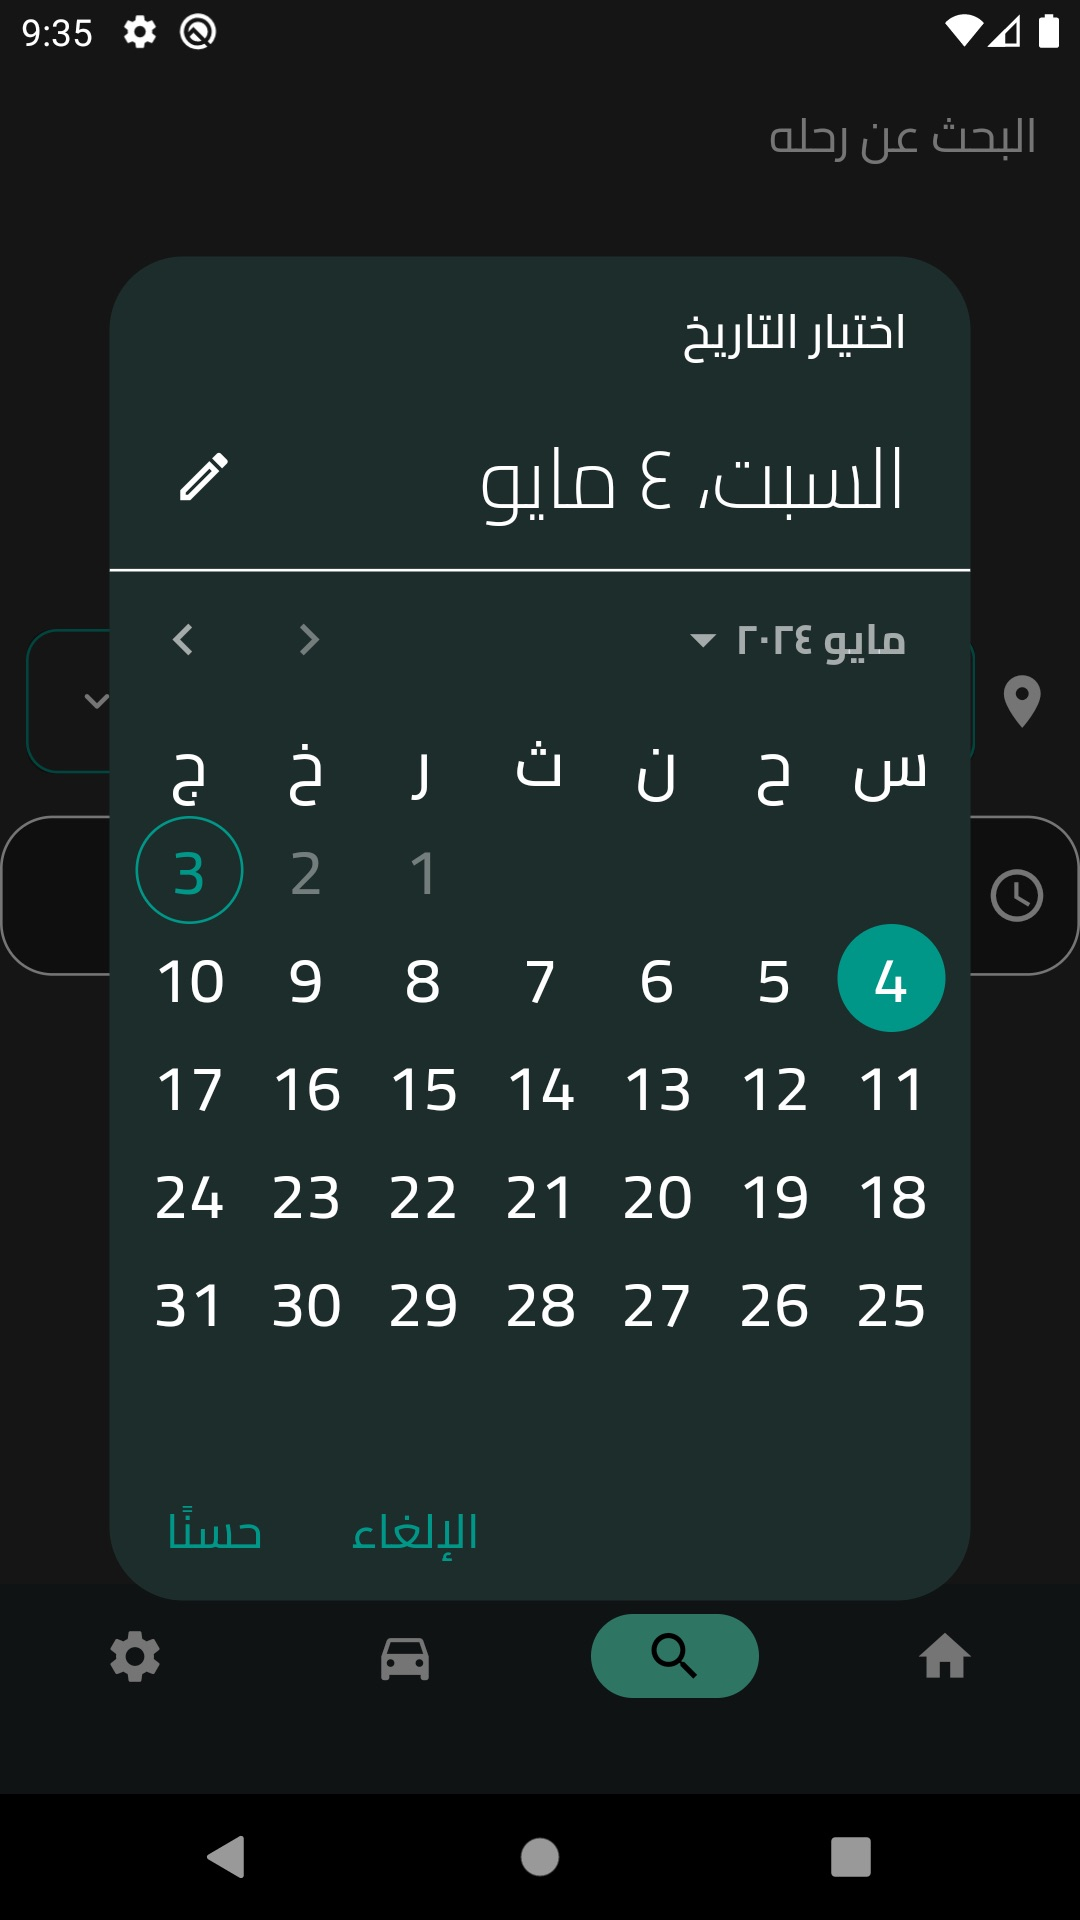
\includegraphics[width=\linewidth]{Images/trip_search_3.png}
                    \caption{Trip Search Result - iOS}
                    \label{fig:trip_search_3}
                \end{subfigure}
                % \label{fig:trip_search}
                \begin{subfigure}{0.31\textwidth}
                    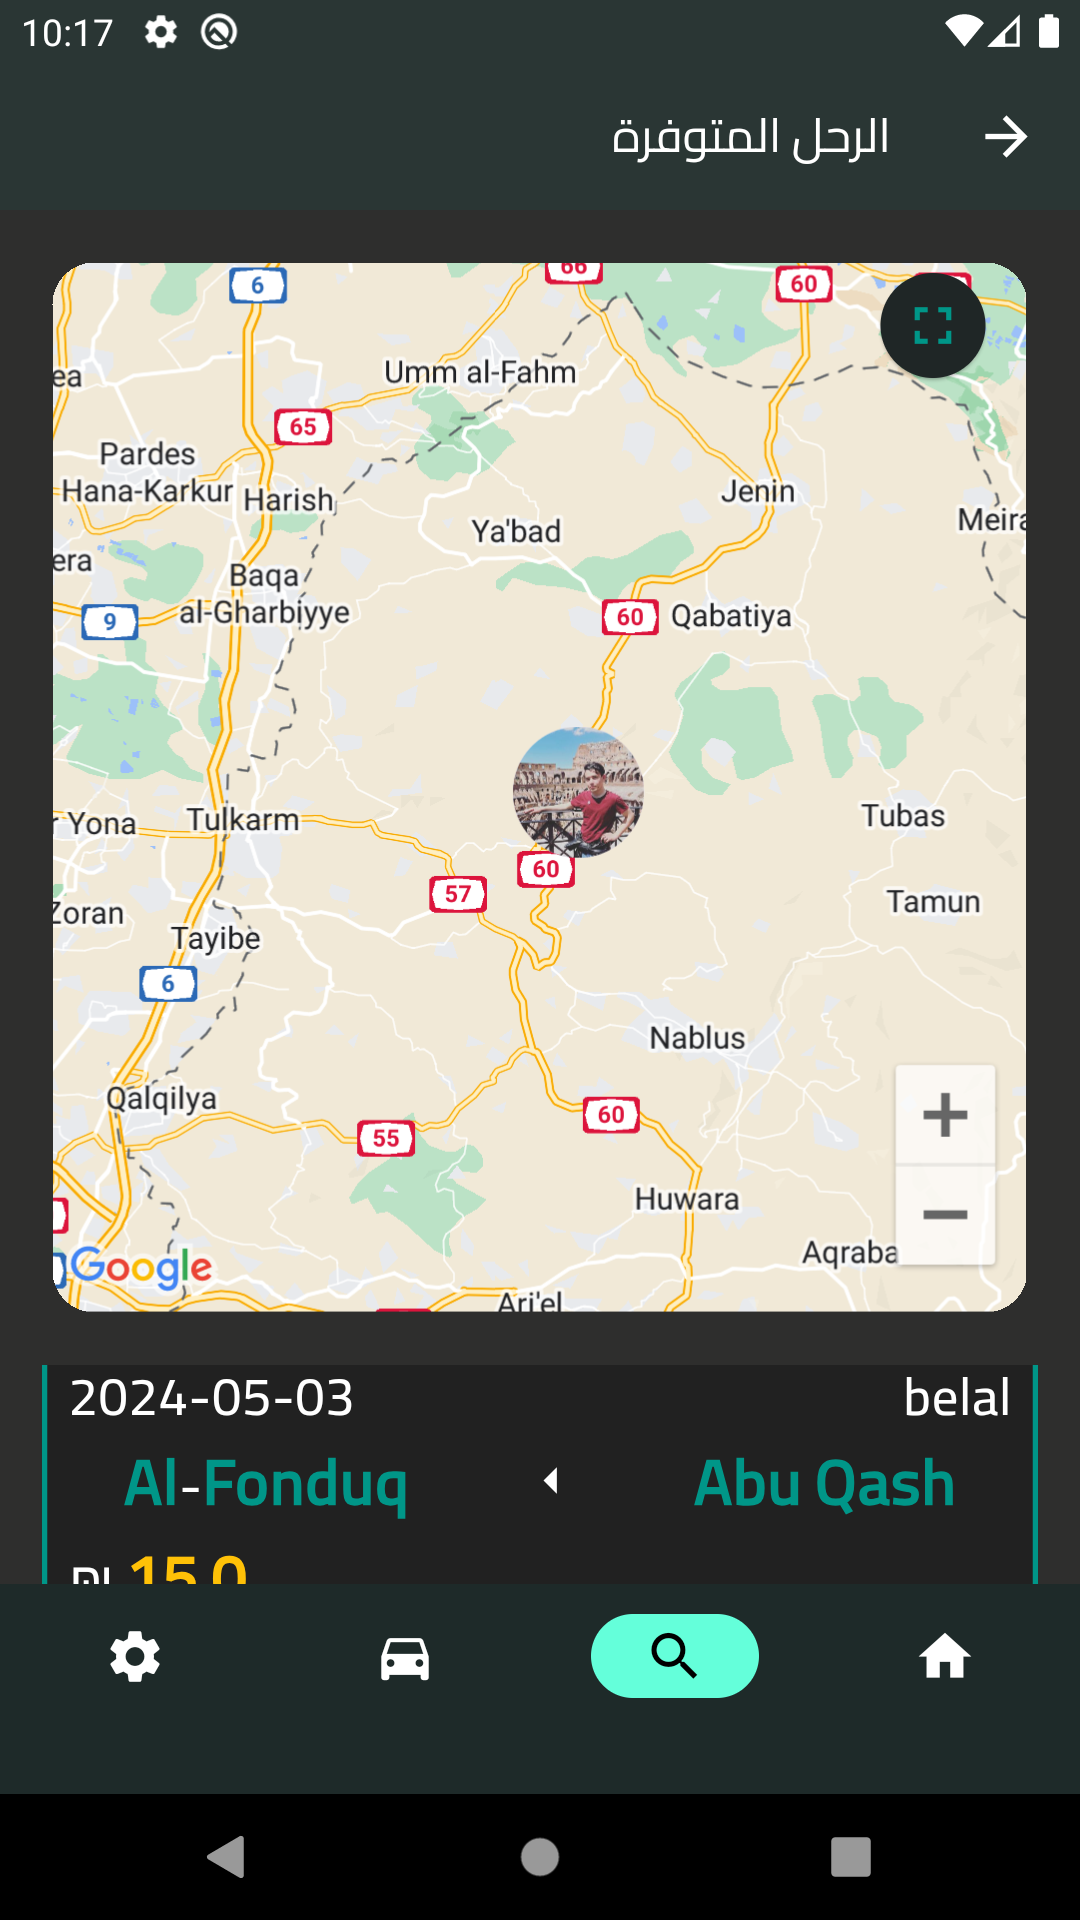
\includegraphics[width=\linewidth]{Images/trip_search_4.png}
                    \caption{Trip Search Result - Android}
                    \label{fig:trip_search_4}
                \end{subfigure}
                \begin{subfigure}{0.31\textwidth}
                    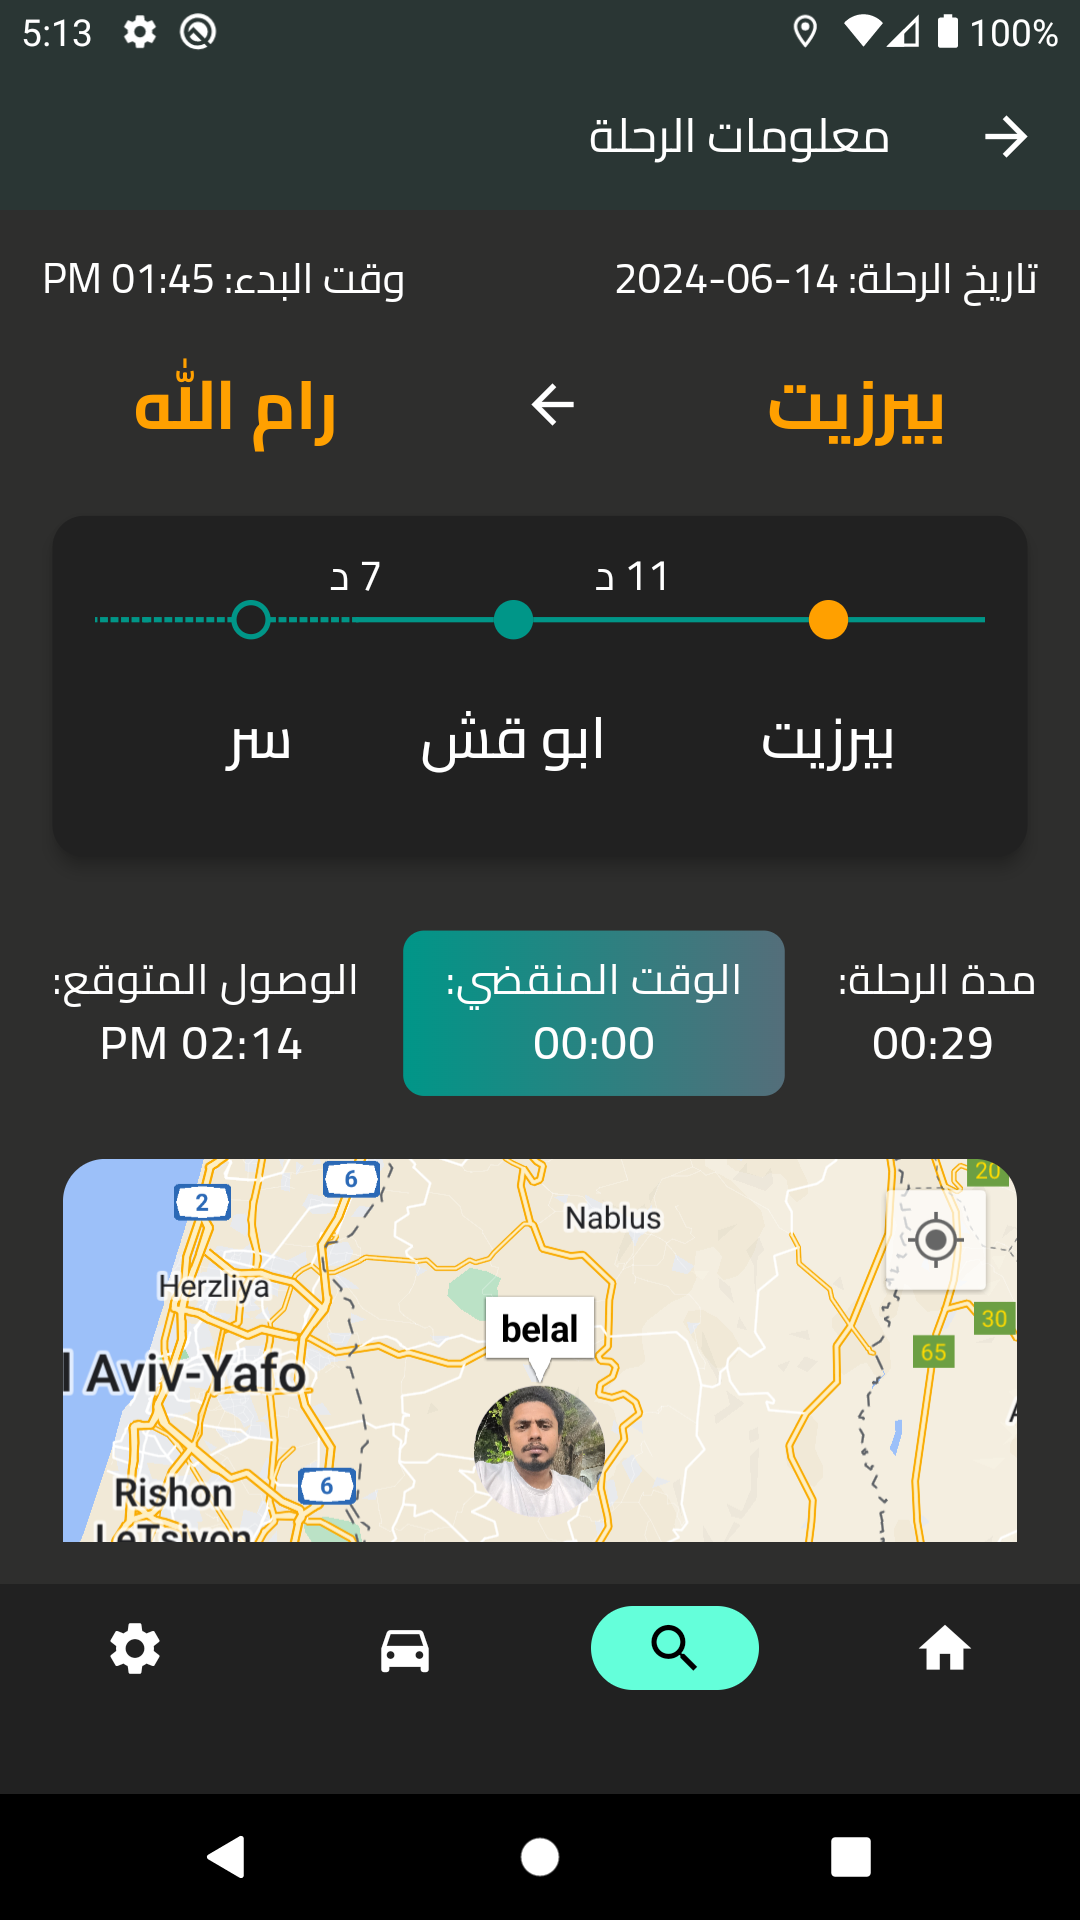
\includegraphics[width=\linewidth]{Images/trip_Detail_screen.png}
                    \caption{Trip Details Screen- Android}
                    \label{fig:trip_details_1}
                \end{subfigure}
                % \caption{Trip Detail Screen}
                \caption{Passenger Trip Search Screens}
                \label{fig:trip_search}
            \end{figure}
        \pagebreak
        \subsection{User Live Location}
            \begin{wrapfigure}{r}{0.45\textwidth}
                \centering
                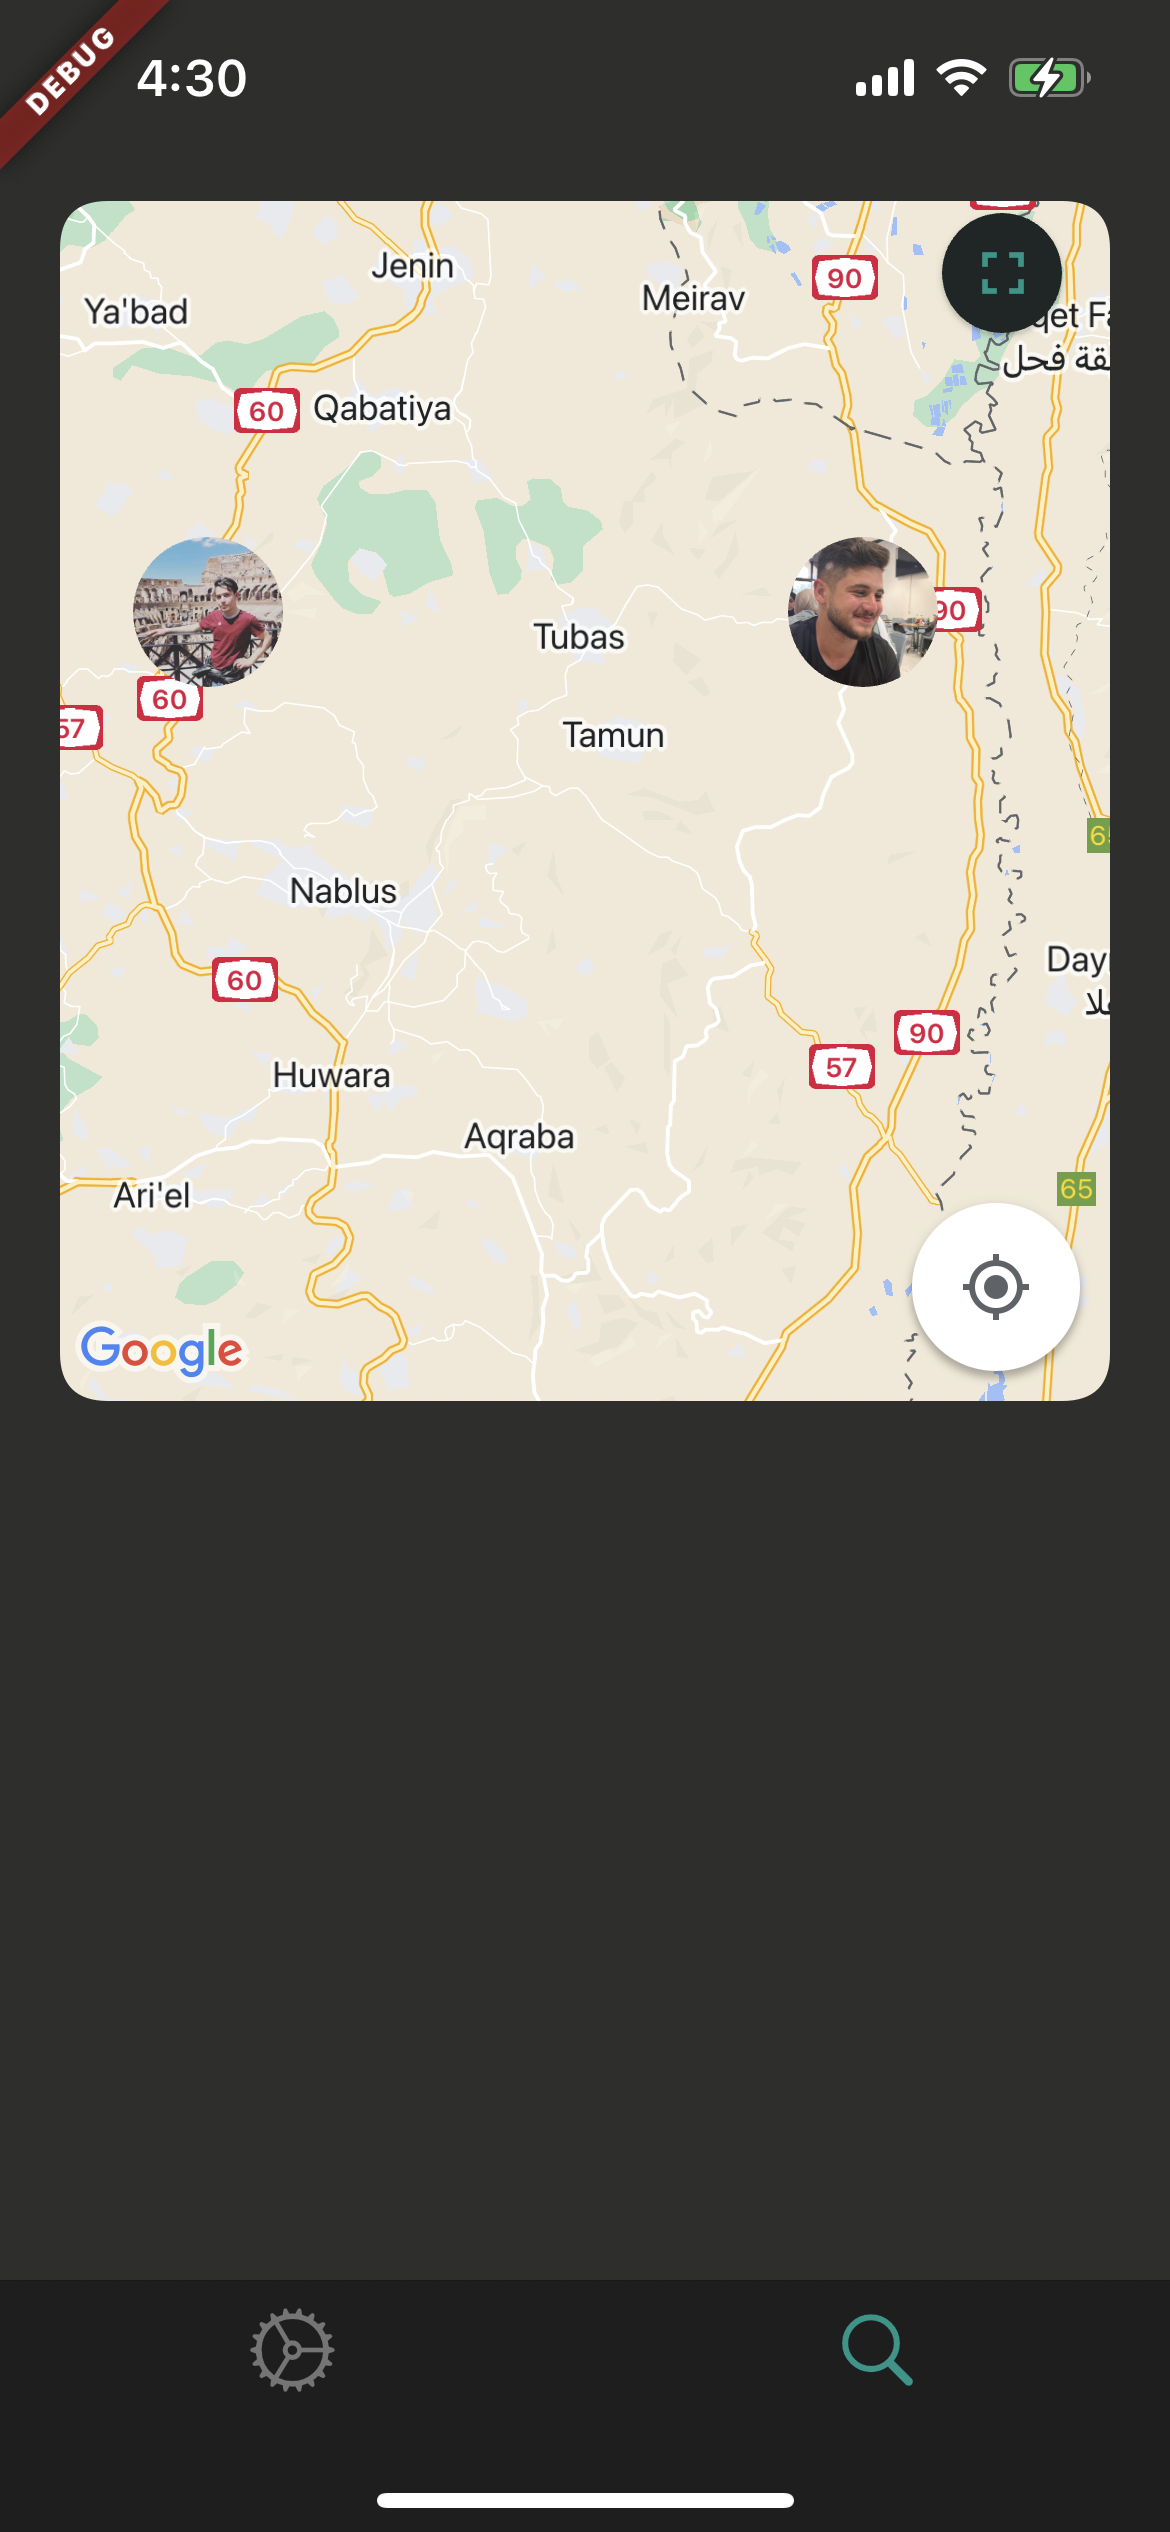
\includegraphics[width=0.65\linewidth]{Images/live_location.png}
                \caption{User Live Location Demo - iOS}
                \label{fig:live_location_demo}
            \end{wrapfigure}
            The app provides features to see the live location of the driver and the passenger. We have configured the app so that it asks for device location permissions on both Android and iOS. We are using Google Maps API to show the live location of the driver and the passenger on an instance of an intractable Google Maps Widget built into the app. We have established a Stream of realtime locations of a group of users stored in FireStore. \ref{fig:live_location_demo} shows the live location feature in action, streaming the location data of users stored in FireStore. We already used this feature to show live location of all relevant drivers to the passenger when booking a trip. We will use this feature for the passenger to track the driver's location and for the driver to see the passenger's location after booking a trip.

        \pagebreak
        \subsection{Profile Picture Picker}
            We have added a functionality for users to add profile pictures using their camera or photo gallery using the Flutter library HL Image Picker \cite{image_picker_lib}. After getting relevant permissions, it allows the user to take/pick photos, crop them, and then set them as their profile picture. 
            \begin{figure}[H]
                \centering
                \begin{subfigure}{0.4\textwidth}
                    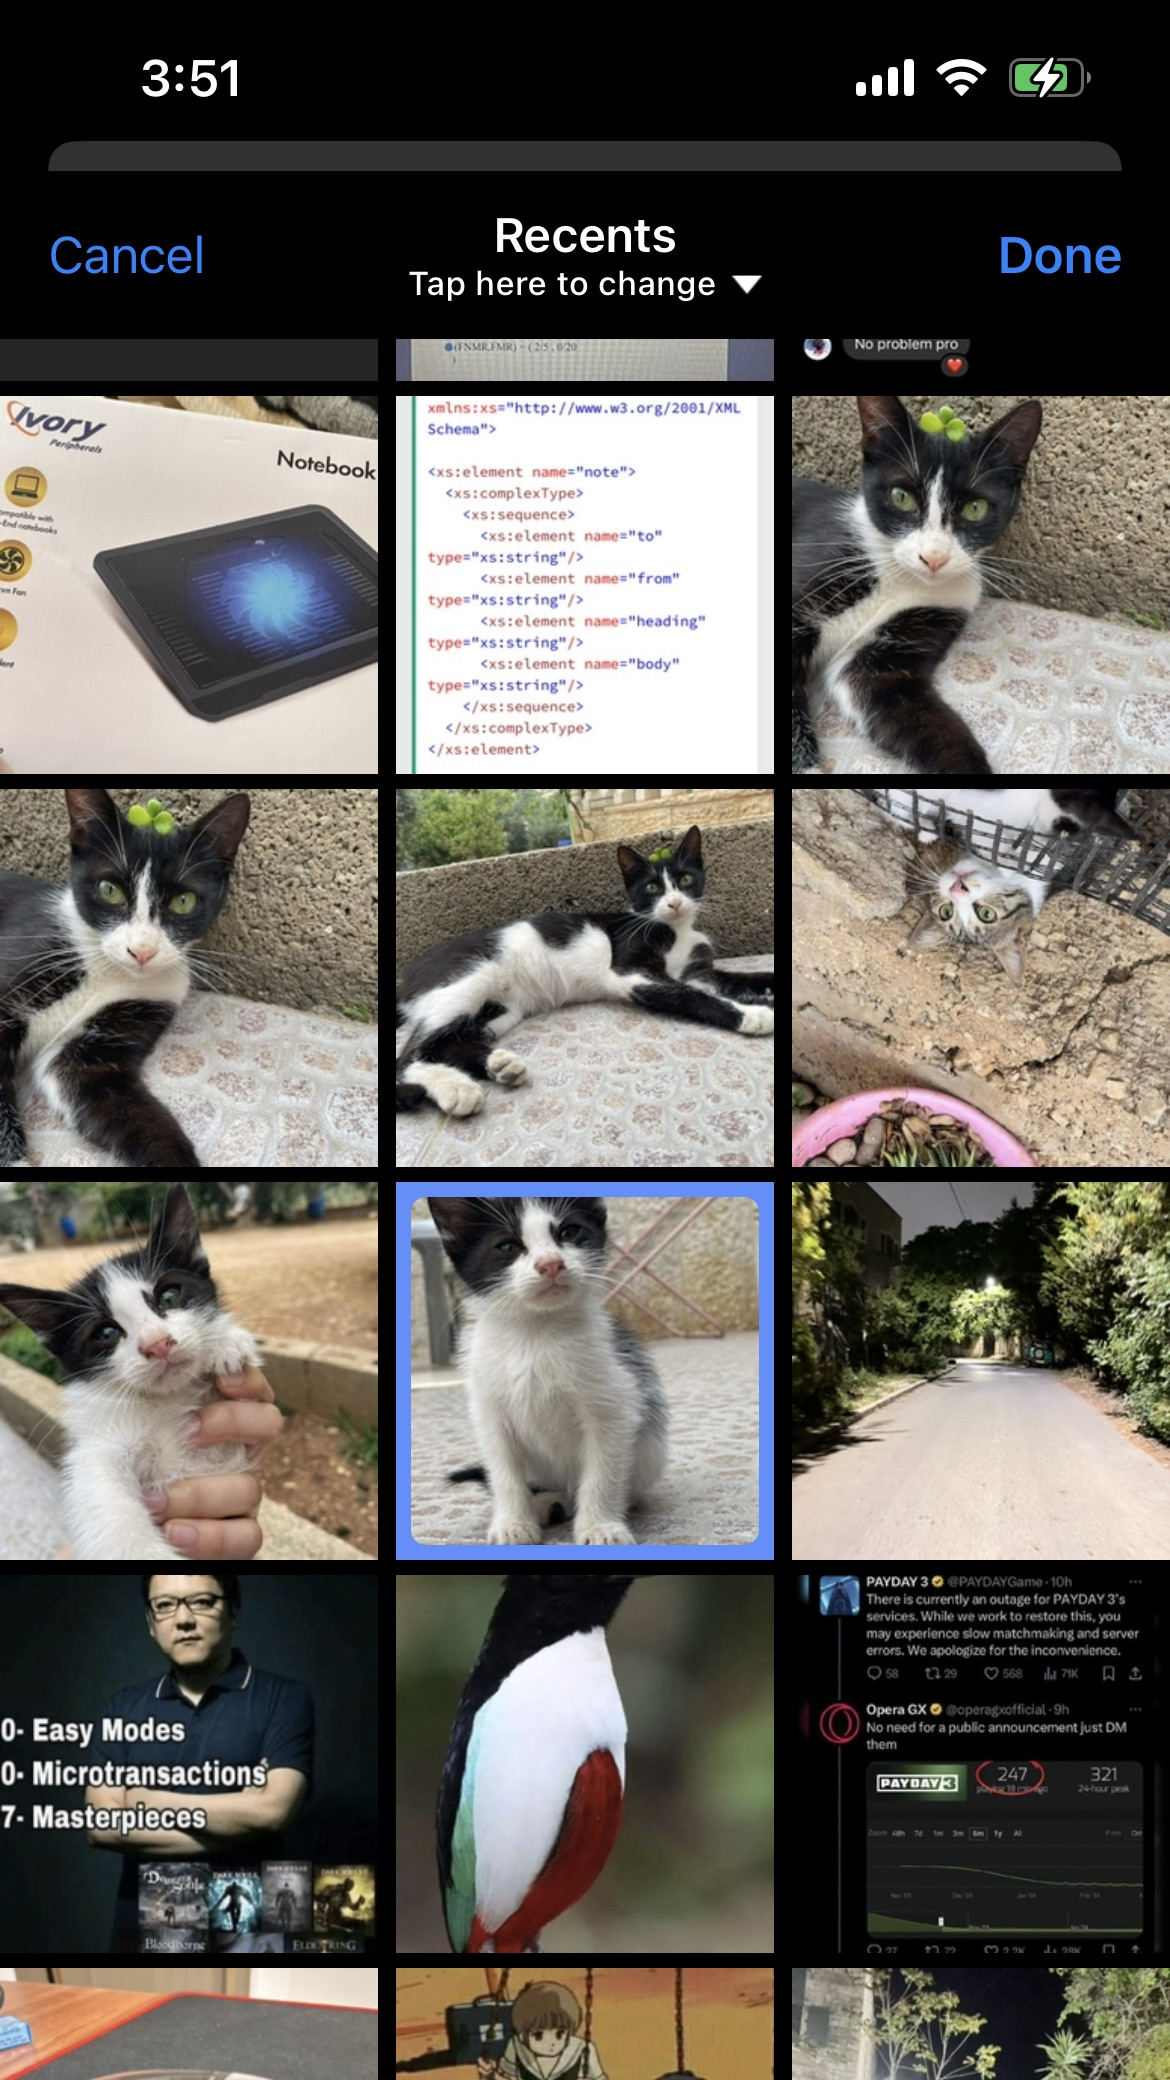
\includegraphics[width=\linewidth]{Images/pfp_select_1.png}
                    \caption{Profile Picture Picker - iOS}
                    \label{fig:pfp_select_1}
                \end{subfigure}
                \begin{subfigure}{0.4\textwidth}
                    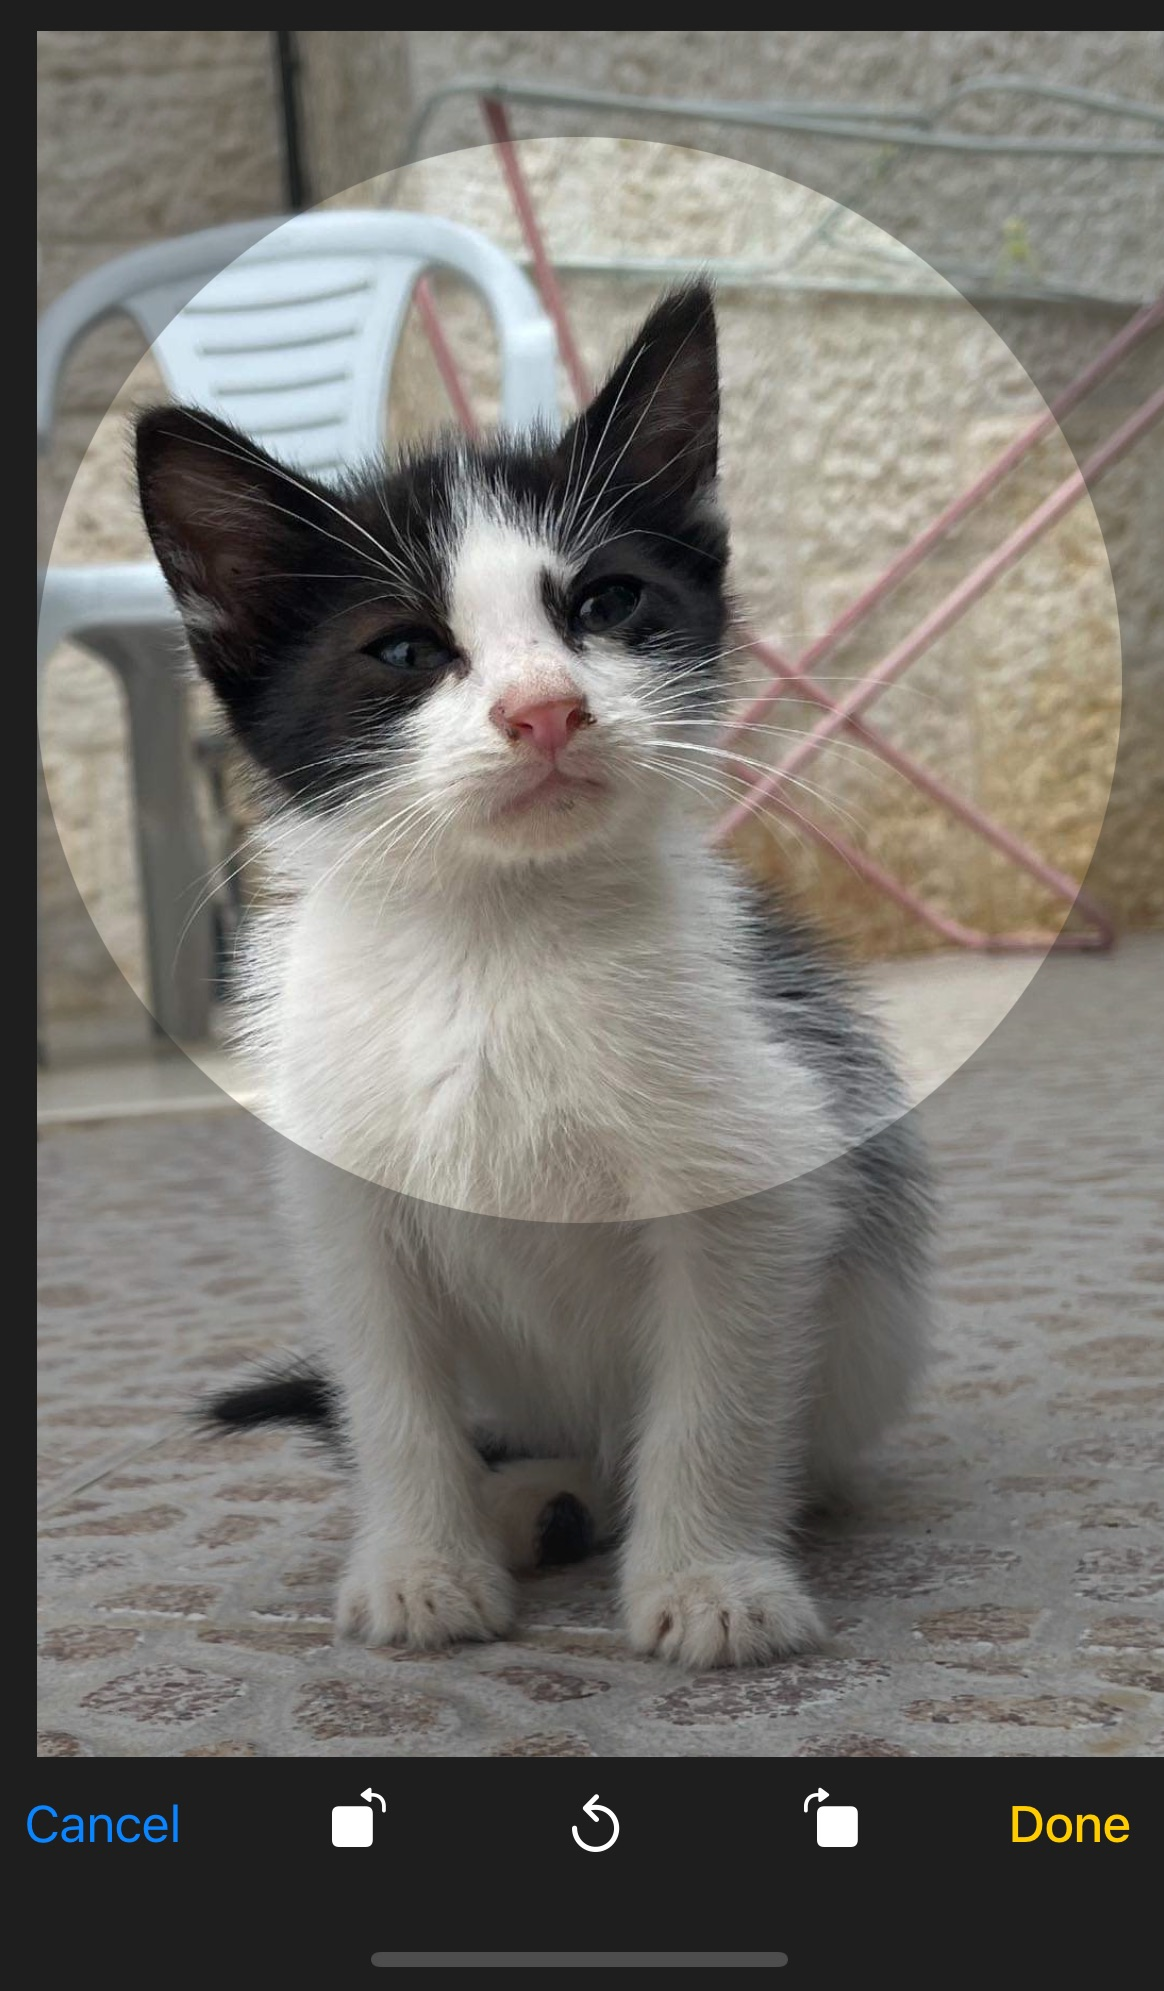
\includegraphics[width=\linewidth]{Images/pfp_select_2.png}
                    \caption{Cont. Profile Picture Picker - iOS}
                    \label{fig:pfp_select_2}
                \end{subfigure}
                \caption{Profile Picture Picker Screens}
                \label{fig:pfp_select}
            \end{figure}

    \pagebreak
    
    \section{Evaluation and Testing}
        During app development with each feature implementation we conducted a series of tests to ensure that the functinality is working as expected and that the app is user friendly. As for each feature, we ensured that the implemented interfaces are simple consistent, conventional and responsive, in addition to achieving their purpose while integrating with the backend of the application.
        And after completing the application conducted system testing of the application which included:
        \subsection{Functional Testing}
            In this stage we tested the functinality of the mobile application, including user interactions, and transactions that may be performed on the application.
            Where for time matter we put some scenarios that the user may perform and conducted a test on it as followed:
            \subsubsection{Downloading the application Test}
                The test was conducted by connecting actual phones instead of emulators and downloading the application directly to them, in which the application was successful downloaded on both android and Iphone mobiles, without any issues.
            \subsubsection{Login and Registration test}
                After downloading the application and running it the main page of the application should appear in which there are several scenarios that can happen:
                \begin{enumerate}
                    \item User is already a member: user can choose to login via email and password or via phoneNo, in which on a successful login attempt he will see the home page.
                    \item New user in which he will click signup button and enter his credintials and information to create an account, on successful signup user is required to verify his email address by entering a link sent to his email, before processing to the home page.
                    \item User is already a member but he forgot his password: in which he will enter his email or phone number, and a message to reset his password will be sent to him.
                    \item User is not connected to the internet: in which the user will be prompted to connect to the internet.
                \end{enumerate}

                \newcolumntype{R}[1]{>{\raggedright\arraybackslash}p{#1}}
                \begin{spacing}{1}
                    \begin{longtable}{| R{2cm}|R{3cm}|R{2cm}|R{2cm}|R{2cm}|R{2cm}|R{2cm}|}
                        \rowcolor{gray} \textbf{Test Case} & \textbf{Inputs} & \textbf{Expected Result} & \textbf{Actual Result} & \textbf{Pass/ Fail} & \textbf{Comments} \\
                        \endfirsthead
                        
                        % \toprule
                        \rowcolor{gray} \textbf{Test Case} & \textbf{Inputs} & \textbf{Expected Result} & \textbf{Actual Result} & \textbf{Pass/ Fail} & \textbf{Comments} \\
                        % \midrule
                        \endhead
                        \caption{Login and Registration Test Cases \label{tab:login_test}}\\
                        
                        \endfoot
                        \caption*{Login and Registration Test Cases (continued)}\\
                        % \bottomrule
                        % \insertTableNotes 
                        \endlastfoot
                        \hline
                        Registration & User credentials: email: lutfi@gmail.com, password: 00456eX@23, etc.. & User is registered and awaits email verification & user is registered and awaits email verification & Pass & Test successful, email verified after the process for further testing\\ 
                        \hline
                        Registration with missing/ incorrect fields & User credentials with weak password and wrong email format & missing/ incorrect fields are marked red and user is asked to correct them & Incorrect/ missing fields are marked red with a prompt message & pass & \\
                        \hline
                        Registration with an already used email & User credentials with email in use & \raggedright{User email already in use message} & User email already in use message& Pass & other correct user credentials are kept as they are he is only alarmed about email\\
                        \hline
                        Login & User email and password & User is logged in and redirected to the home page & User is logged in and redirected to the home page & Pass & \\
                        \hline
                        Login with wrong email or password & User email and password & User is prompted to enter correct email or password & User is prompted to enter correct email or password & Pass & \\
                        \hline
                        Login with forgot password & Email address & Email is sent to reset the password if account exists& Email is sent to reset the password if account exist &Pass & password is reset via the link\\
                        \hline
                        Login/ registration without internet connection & User credentials & User is prompted to connect to the internet & User is prompted to connect to the internet & Pass & \\
                        \hline
                    \end{longtable}
                \end{spacing}
                
                % TODO: a table of Login Test cases don't 
            \subsubsection{Search A Trip test}
                After successful login, user can search for a trip by entering the search trip screen, entering required filed: such as starting station, end station, datetime of the trip and number of passengers.
                then clicking the search button in which different results can appear:
                \begin{enumerate}
                    \item finding matching trips, in which a split screen is shown with the map and driver last seen locations on it, and a card list in which trip informations are listed.
                    \item No matching trip is found/ all matching trips are full, in which the user is prompted and told that no matching trips are found.
                    \item User missed to enter a required field, in which the user is prompted to enter the missing field.
                \end{enumerate}

                \pagebreak

                \begin{spacing}{1}               
                    \begin{longtable}{| R{2cm}|R{3cm}|R{2cm}|R{2cm}|R{2cm}|R{2cm}|R{2cm}|}
                        \rowcolor{gray} \textbf{Test Case} & \textbf{Inputs} & \textbf{Expected Result} & \textbf{Actual Result} & \textbf{Pass/ Fail} & \textbf{Comments} \\
                        
                        \endfirsthead
                        \endhead
                
                        \endfoot
                        \endlastfoot
                        \hline
                        Search for a trip & User inputs (eg: start station: Ramallah, end station: Birzeit, date: 2024-6-24, passengers: 2) & User is shown a list of matching trips how are from the same date up to the next 48 hours & List of matching trips which have available seats are shown & Pass & Trips and trip drivers are shown both on map and as a list in a split screen\\
                        \hline
                        Search for a trip with no matching trips & User inputs (eg: start station: Ramallah, end station: Qalqilya, date: 2024-6-24, passengers: 2) & User is prompted that no matching trips are found & User is prompted that no matching trips are found & Pass & full trips are considered a non-match\\
                        \hline
                        Search for a trip with missing fields & User inputs (eg: start station: Ramallah, end station: Birzeit, date: 2024-6-24) & User is prompted to enter the missing field & User is prompted to enter the missing field & Pass & \\
                        \hline
                        Search for a trip with same start and end station & User inputs (eg: start station: Ramallah, end station: Ramallah, date: 2024-6-24, passengers: 2) & User is prompted that start and end station can't be the same & User is prompted that start and end station can't be the same & Pass & \\
                        \hline
                        Search for a trip with no internet connection & User inputs (eg: start station: Ramallah, end station: Birzeit, date: 2024-6-24, passengers: 2) & User is prompted to connect to the internet & User is prompted to connect to the internet & Pass & User session is locally stored, including stations and are updated when the internet connection is established\\
                        \hline
                        \caption{Search A Trip Test Cases \label{tab:search_trip_test}}\\

                    \end{longtable}
                \end{spacing}

                \subsubsection{Book a Trip test}
                After finding a matching trip, user can book a trip by clicking on the trip card, in which the trip details are shown, and the user can click on the book button, in which the user will be prompted to enter his payment method, and after successful payment the user will be redirected to the home page.
                in which different scenarios can happen:
                \begin{enumerate}
                    \item User has a payment method, in which the user will be redirected to the home page.
                    \item User has no payment method, in which the user will be prompted to enter a payment method.
                    \item User returned to the previous page, in which the trip search screen is shown again.
                \end{enumerate}
                On each stage the user has choosen a certain trip, and is shown the trip details screen, in which the user can see the driver information, and trip rules, estimated time for the trip, the full path of the trip (trip stations), price, and trip state(started, pending)
                On successful stage the driver is notified about the booking request, and the passenger is notified about the driver response when it happens.
                \begin{spacing}{1}
                    \begin{table}[H]
                        \centering
                        \label{tab:login_test}
                        \begin{tabularx}{\textwidth}{| R{2cm}|R{3cm}|R{2cm}|R{2cm}|R{2cm}|R{2cm}|R{2cm}|}
                            \hline
                            \rowcolor{gray} \textbf{Test Case} & \textbf{Inputs} & \textbf{Expected Result} & \textbf{Actual Result} & \textbf{Pass/ Fail} & \textbf{Comments} \\
                            % Test Case & inputs & Expected Result & Actual Result & Pass/Fail & Comments \\
                            \hline
                            Book a trip & User clicks on a trip card & User is prompted to enter payment method & User is prompted to enter payment method & Pass & on successful payment user request is sent to the driver and driver is notified\\
                            \hline
                            Book a trip with no payment method & User clicks on a trip card & User is prompted to enter payment method & User is prompted to enter payment method & Pass & \\
                            \hline
                            Cancel booking page & User clicks on a trip card & User is redirected to the trip details page & User is redirected to the trip details page & Pass & \\
                            \hline
                        \end{tabularx}
                        \caption{Book A Trip Test Cases}
                    \end{table}
                \end{spacing}


            \subsubsection{Create a Trip for Driver test}
                After successful login, if user is registered as driver he can create a trip by entering the create trip screen, entering required filed: such as starting station, end station, datetime of the trip, number of passengers, and price of the trip.
                then clicking the create button in which different results can appear:
                \begin{enumerate}
                    \item Trip is created successfully, in which the user is redirected to the trip details page.
                    \item User missed to enter a required field, in which the user is prompted to enter the missing field.
                    \item User returned to the previous page, in which the home page is shown again.
                \end{enumerate}

                \begin{spacing}{1}
                    \begin{table}[H]
                        \centering
                        \label{tab:login_test}
                        \begin{tabularx}{\linewidth}{| R{2cm}|R{3cm}|R{2cm}|R{2cm}|R{2cm}|R{2cm}|R{2cm}|}
                            \hline
                            \rowcolor{gray} \textbf{Test Case} & \textbf{Inputs} & \textbf{Expected Result} & \textbf{Actual Result} & \textbf{Pass/ Fail} & \textbf{Comments} \\
                            \hline
                            Create a trip & User inputs (eg: start station: Ramallah, end station: Birzeit, start-time: 2024-6-24:12:00PM, passengers: 2, price: 10) & User is redirected to the trip details page & User is redirected to the trip details page & Pass & option for the driver is to start the trip if its 30 minutes away from the start time\\
                            \hline
                            Create a trip with missing fields & User inputs (eg: start station: Ramallah, end station: Birzeit, start-time: 2024-6-24:12:00PM, passengers: 2) & User is prompted to enter the missing field & User is prompted to enter the missing field and field is marked red & Pass & \\
                            \hline
                            Create a trip with same start and end station & User inputs (eg: start station: Ramallah, end station: Ramallah, start-time: 2024-6-24:12:00PM, passengers: 2, price: 10) & User is prompted that start and end station can't be the same & User is prompted that start and end station can't be the same & Pass & \\
                            \hline
                            Create a trip with no internet connection & User inputs (eg: start station: Ramallah, end station: Birzeit, start-time: 2024-6-24:12:00PM, passengers: 2, price: 10) & User is prompted to connect to the internet & User is prompted to connect to the internet & Pass & User session is locally stored, including stations and are updated when the internet connection is established\\
                            \hline
                        \end{tabularx}
                        \caption{Create A Trip Test Cases}
                    \end{table}
                \end{spacing}

            \subsubsection{Accepting a Trip Request test}
                After a passenger books a trip, the driver is notified about the booking request, and the driver can accept or decline the request. The driver can accept the request by clicking on the notification, in which the driver is redirected to the trip requests page, and then accepting/declining the request, and the passenger is notified about the driver response.

                \begin{spacing}{1}
                    \begin{table}[H]
                        \centering
                        \label{tab:login_test}
                        \begin{tabularx}{\linewidth}{| R{2cm}|R{3cm}|R{2cm}|R{2cm}|R{2cm}|R{2cm}|R{2cm}|}
                            \hline
                            \rowcolor{gray} \textbf{Test Case} & \textbf{Inputs} & \textbf{Expected Result} & \textbf{Actual Result} & \textbf{Pass/ Fail} & \textbf{Comments} \\
                            \hline
                            Accept a trip request & Driver clicks on a trip request notification & Driver is redirected to the trip requests page & Driver is redirected to the trip requests page & Pass & nottification is sent to the passenger with updates info\\
                            \hline
                            Decline a trip request & Driver clicks on a trip request notification & Driver is redirected to the trip requests page & Driver is redirected to the trip requests page & Pass & notification is sent to the passenger with updates info\\
                            \hline
                        \end{tabularx}
                        \caption{Accepting A Trip Request Test Cases}
                    \end{table}
                \end{spacing}

        \subsubsection{Live Location test}
            As for the live location feature, the user can see the live location of the driver and the passenger, in which the user can see the live location of the driver and the passenger on an instance of an intractable Google Maps Widget built into the app.
            For this feature we tested the working of the live location feature by running the application in a test screen environment, in which the live location of two users where shown on the map, and in which they were updated in real time and synchronized with the location in the database.
            As for this feature its not specific to a certain user, but it is a general feature that can be used by all users. and we saw that an evaluation test as the one we conducted is enough to ensure the working of the feature
        \subsection{Performance Testing}
            For this stage we wanted to test the performance of the application, in which we tested the application on different devices, where we found that the application worked as expected on both android and iOS devices, and that the application was responsive and fast, and that the application was able to handle the different functionalities and features that it has.
            For the load testing we used a firebase database which is a database hosted by google, and is able to handle a large number of requests, and operations and is able to scale with the application.
            in addition we validated the response time of the application, and asked different users to use the application and give us feedback on the application, in which we validated that the application response time was acceptable.
            As for this seciton we assured that the application is able to perform well and it can handle the different requests and operations that it was given.
        \subsection{Usablity Testing}
        As for the usability testing, we conducted a series of tests to ensure that the application is user friendly, and that users can easily navigate through the application, and that the user can easily find the different features and functionalities that the application has, in which we asked the different users, who we have gaven the application to, to give us feedback on the application, and to tell us if they found the application easy to use, and if they were able to find the different features and functionalities that the application has.
        And whether they had any problems or misconceptions while using the application. this part was done in parralel with the other testing stages, as the same users who were testing the application were asked to give us feedback on the application.
    \pagebreak
    \section{Conclusion}
        This project has successfully developed, the Carpal Ridesharing App, tailored to the unique road conditions and transportation needs in Palestine, where thousands of people rely on various forms of transportation for their daily commutes. Recognizing the challenges with conventional transportation methods—such as issues with time, availability, and comfort—our app provides a viable alternative that addresses these problems effectively.

        The CarPal Ridesharing App allows anyone with a driver's license and a car to offer rides to others, facilitating pickups along their routes at any time. This innovative solution helps reduce the costs of commuting, minimizes the number of trips required, and significantly cuts down on waiting time. It is designed to be both affordable and easily accessible through a user-friendly mobile app.

        With our app, users can create accounts and become verified drivers, enabling them to schedule trips, or they can search for rides as passengers. Passengers have the convenience of booking and paying through the app. At the conclusion of each trip, both passengers and drivers can provide feedback, fostering a community of trust and reliability.

        We believe that Carpal will significantly improve the daily commute for many people and hope it will soon become an integral part of Palestine's transportation ecosystem.
        
    \section{Future Work}
        % \begin{enumerate}
        %     \item adding more stations
        %     \item chat
        %     \item payment
        %     \item Roads status Telegram channel integration
        %     \item Sharing trip link
        %     \item Learned trip time prediction
        %     \item Settings page for font
        %     \item More languages
        % \end{enumerate}
        %TODO: add future work

        % \afterpage{ % used with clear page to add a page break before references. Figures and tables become centered without this
        % }

    % \pagebreak

    % \clearpage % page break doesn't add space before the references page so this needed
    \printbibliography

\end{document} % This is the end of the document

